\documentclass[supercite]{Experimental_Report}

\title{~~~~~~新生实践课~~~~~~}
\author{彭嘉炜}
\school{计算机科学与技术学院}
\classnum{CS2110}
\stunum{U202115630}
\instructor{} % 李平、孙伟平、范晔斌、陈加忠
\date{2021年11月11日}
\hypersetup{
colorlinks=true,
linkcolor=black
}
\usepackage{listings}
\usepackage{algorithm, multirow}
\usepackage{algpseudocode}
\usepackage{amsmath}
\usepackage{makecell}
\usepackage{amsthm}
\usepackage{framed}
\usepackage{mathtools}
\usepackage{subcaption}
\usepackage{xltxtra} %提供了针对XeTeX的改进并且加入了XeTeX的LOGO, 自动调用xunicode宏包(提供Unicode字符宏)
\usepackage{bm}
\usepackage{tikz}
\usepackage{tikzscale}
\usepackage{pgfplots}
%\usepackage{enumerate}

\pgfplotsset{compat=1.16}
\definecolor{dkgreen}{rgb}{0,0.6,0}
\definecolor{gray}{rgb}{0.5,0.5,0.5}
\definecolor{mauve}{rgb}{0.58,0,0.82}

\lstset{frame=tb,
  language=Go,
  aboveskip=3mm,
  belowskip=3mm,
  showstringspaces=false,
  columns=flexible,
  basicstyle={\small\ttfamily},
  numbers=none,
  numberstyle=\tiny\color{gray},
  keywordstyle=\color{blue},
  commentstyle=\color{dkgreen},
  stringstyle=\color{mauve},
  breaklines=true,
  breakatwhitespace=true,
  tabsize=3
}
\newcommand{\cfig}[3]{
  \begin{figure}[htb]
    \centering
    \includegraphics[width=#2\textwidth]{images/#1.tikz}
    \caption{#3}
    \label{fig:#1}
  \end{figure}
}

\newcommand{\sfig}[3]{
  \begin{subfigure}[b]{#2\textwidth}
    \includegraphics[width=\textwidth]{images/#1.tikz}
    \caption{#3}
    \label{fig:#1}
  \end{subfigure}
}

\newcommand{\xfig}[3]{
  \begin{figure}[htb]
    \centering
    #3
    \caption{#2}
    \label{fig:#1}
  \end{figure}
}

\newcommand{\rfig}[1]{\autoref{fig:#1}}
\newcommand{\ralg}[1]{\autoref{alg:#1}}
\newcommand{\rthm}[1]{\autoref{thm:#1}}
\newcommand{\rlem}[1]{\autoref{lem:#1}}
\newcommand{\reqn}[1]{\autoref{eqn:#1}}
\newcommand{\rtbl}[1]{\autoref{tbl:#1}}

\algnewcommand\Null{\textsc{null }}
\algnewcommand\algorithmicinput{\textbf{Input:}}
\algnewcommand\Input{\item[\algorithmicinput]}
\algnewcommand\algorithmicoutput{\textbf{Output:}}
\algnewcommand\Output{\item[\algorithmicoutput]}
\algnewcommand\algorithmicbreak{\textbf{break}}
\algnewcommand\Break{\algorithmicbreak}
\algnewcommand\algorithmiccontinue{\textbf{continue}}
\algnewcommand\Continue{\algorithmiccontinue}
\algnewcommand{\LeftCom}[1]{\State $\triangleright$ #1}

\newtheorem{thm}{定理}[section]
\newtheorem{lem}{引理}[section]

\colorlet{shadecolor}{black!15}

\theoremstyle{definition}
\newtheorem{alg}{算法}[section]

\def\thmautorefname~#1\null{定理~#1~\null}
\def\lemautorefname~#1\null{引理~#1~\null}
\def\algautorefname~#1\null{算法~#1~\null}

\begin{document}

\maketitle

\clearpage

\pagenumbering{Roman}

\tableofcontents[level=2]
\clearpage

\pagenumbering{arabic}

\section{问题定义}

\subsection{项目背景及意义}

\subsubsection{项目背景}

如今Linux系统被广泛使用,我们需要一种中心化的机制用于搜索以及安装软件。然而软件通常需要存放在存储库里,
并通过包的形式进行分发。我们需要一个方便好用的包管理系统来安装更新包文件。当然我们也可以通过一些现有的开发好的软件商店进行软件的安装,他们的优势是
具有一个图形化的界面,可以使用鼠标点击安装,在使用上更加人性化,现有的应用商店有 GNOME Software, Discover, 
AppCenter等,虽然他们都已经有了十分成熟的系统机制,但是依然或多或少的缺点,
例如GNOME Software和Discover和桌面环境深度绑定,因此我们决定开发一款基于electron的跨发行版跨桌面的的应用商店,
为用户提供更加美观,人性化的界面如图\ref{UnixAppstore}。

同时维护我们自己的软件源,一方面提供镜像的功能,一方面则是方便开发者进行软件的上传。
\begin{figure}[ht]
    \centering
    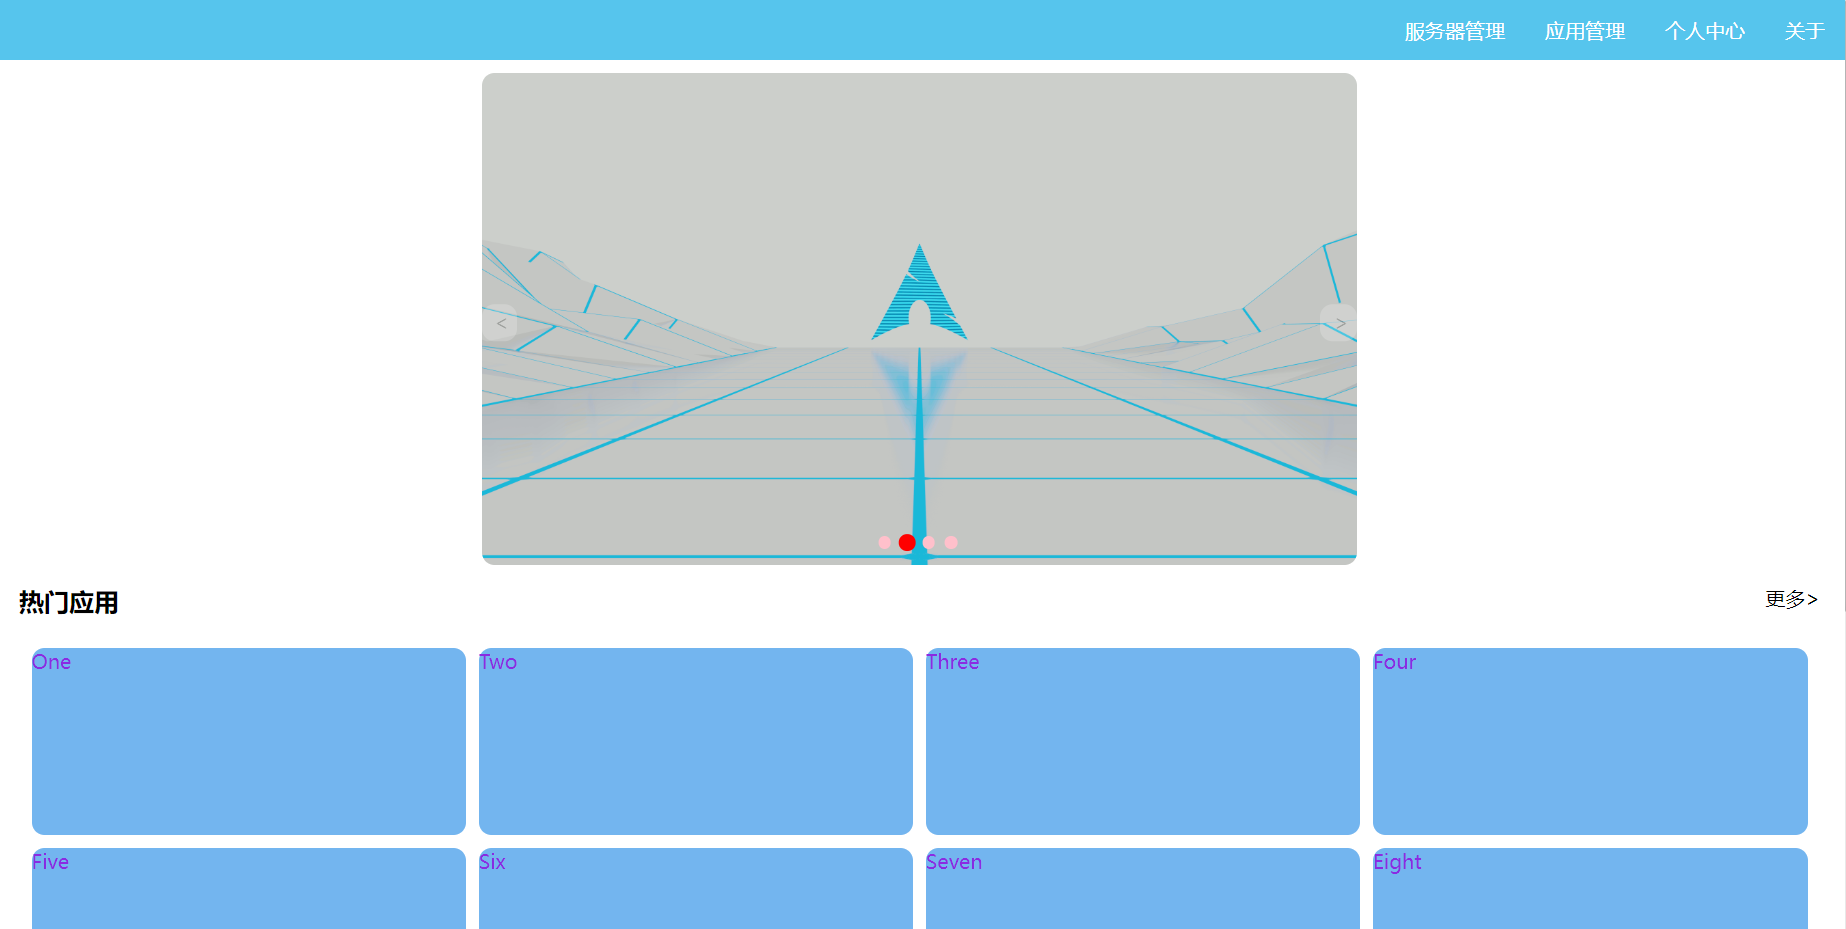
\includegraphics[scale=0.25]{./images/UnixAppstore}
    \caption{主界面}
	\label{UnixAppstore}
\end{figure}

\subsubsection{项目意义}

在当今的外部环境下,越来越多的关键行业从业人员选择使用开源的linux作为自己的工作环境,项目的意义在于降低用户使用linux的门槛,
为用户提供图形化的软件安装界面,不需要接触命令行。同时用户可以在不同的发行版上使用此项目,不需要了解不同发行版上的包管理工具和包命名风格。

对于开发者而言,我们提供一个软件上传平台,方便开发者在其中发行他们的软件,可以被该项目的用户所使用,在完成上传后,还可以对软件包进行持续的维护,维护自主可控的软件源。

\subsection{项目基本目标}

1. 本项目致力于开发一款跨平台的应用,在不同的Linux发行版本都可以进行软件包的下载与安装,在不同的发行版下调用不同的包管理工具进行软件管理。

2. 在安装软件的时候可以选择在本机进行安装,或者是在自己的服务器上进行安装,此外我们还需要在本地连接远程的终端进行更加复杂的操作。

3. 为开发者提供上传软件的功能,上传的软件包可以被用户所搜索。

4. 开发后台管理界面,管理者需要对上传的软件包进行认证和分类等操作。

5. 可以实现镜像的功能,将远程的软件源同步到我们部署的服务器上 



最终实现的项目如图\ref{all}所示,构建一个从发行版到服务对象的桥梁。
\begin{figure}[ht]
    \centering
    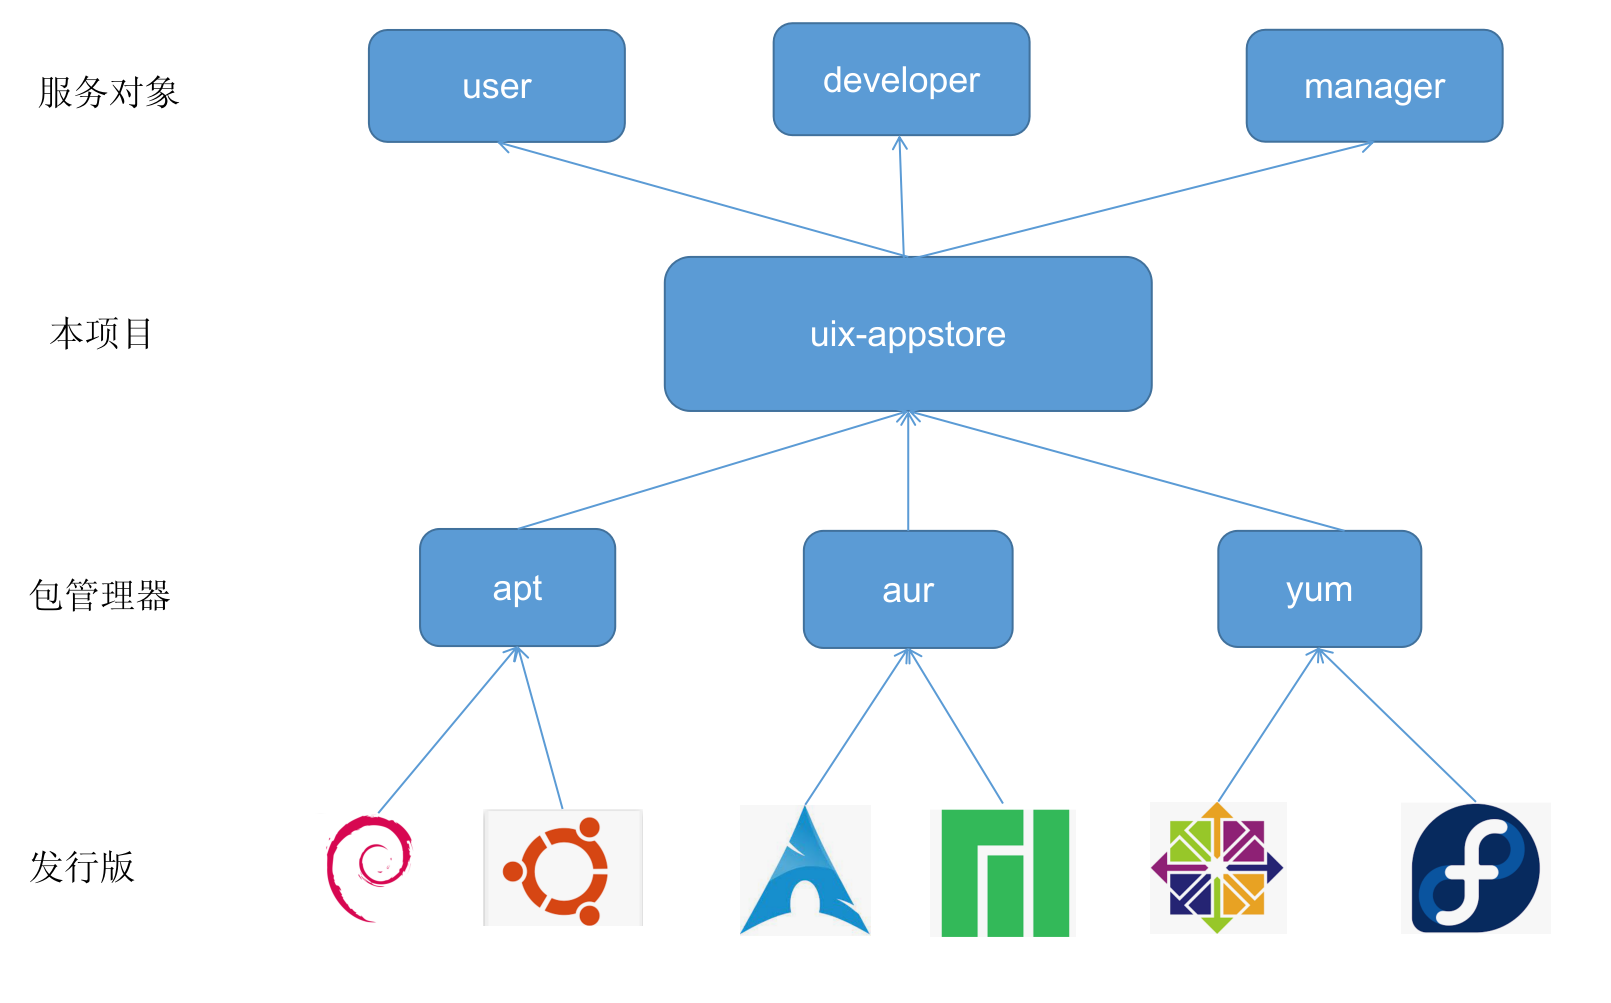
\includegraphics[scale=0.5]{./images/all.png}
    \caption{项目目标}
	\label{all}
\end{figure}


\newpage
\subsection{可行性分析}
\subsubsection{用户基础}

linux操作系统在服务器端有着举足轻重的作用,根据图\ref{linux}所示在2021年的调查中其占比达
到了20.9\%,随之而来的是庞大的用户基数,同时在国内出现了一批deepin, 优麒麟等优秀的发行版,很多
关键行业人员也选择使用这些国产系统来保证"自主可控"。
\begin{figure}[ht]
    \centering
    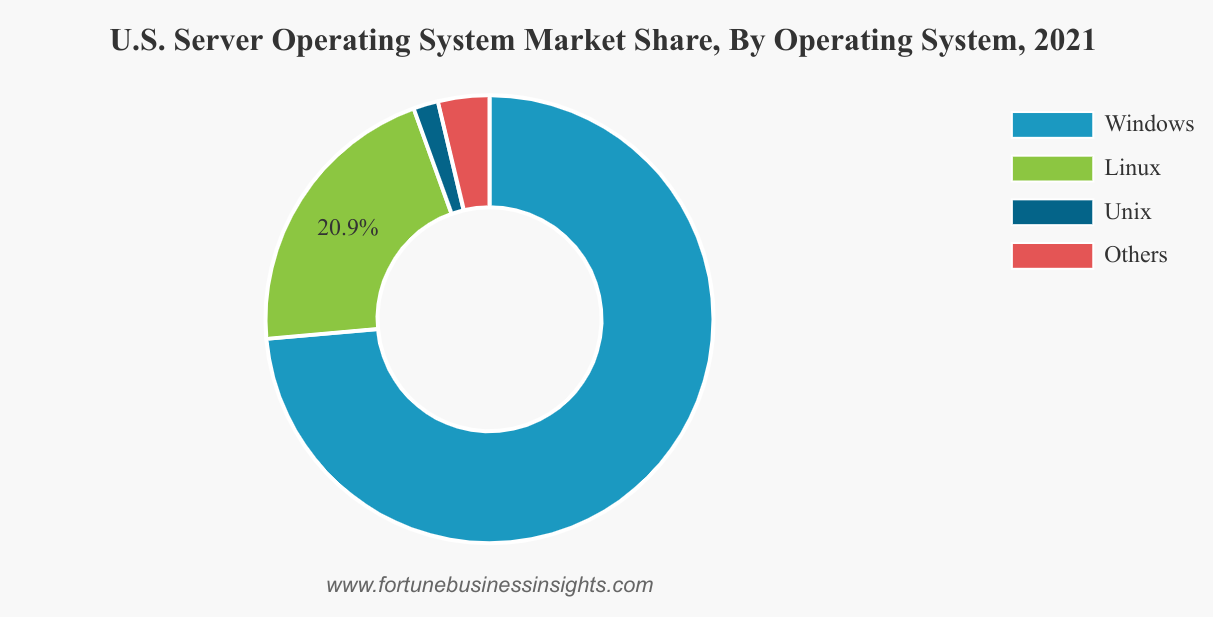
\includegraphics[scale=0.5]{./images/linux_par.png}
    \caption{操作系统市场份额}
	\label{linux}
\end{figure}

\subsubsection{技术可行性分析}
当前最流行的跨平台开发框架是electron,如vscode, yesplaymusic都是基于electron实现的优秀应用,在不同的操作系统,
不同的发行版上都能运行,所以我们在框架选择上选择使用electron进行开发。

在后端选择上,当前我们选择使用go进行开发,进行用户的身份认证和软件的上传,后期准备转入java,因为相对于go,java有着
有着更加完整的生态和更多丰富的优秀案例。

在包的管理上,我们根据不同的系统调用不同的包管理工具,再使用shell和js进行交互。

设计技术框架如图\ref{tech}所示,前端暂时使用原生的js没有使用React/Vue等框架,目前正在使用React对其进行重构中,
后端的技术选型如表\ref{back}所示
\newpage

\begin{table}[!h]
	\centering
	\caption{后端技术选型}
	\label{back}
	\setlength{\tabcolsep}{7mm}{
	\begin{tabular}{cc}
		\toprule
		模块& 选型方案\\
		\midrule
		数据库& postgresql\\
		ORM & xorm \\
		web框架 & iris\\
		日志框架 & logrus \\
		同步工具 & go-git/go-rsync/resty\\
		\bottomrule
	\end{tabular}
	}
\end{table}
最终呈现出的前后端框架如图\ref{tech} 所示

\begin{figure}[ht]
    \centering
    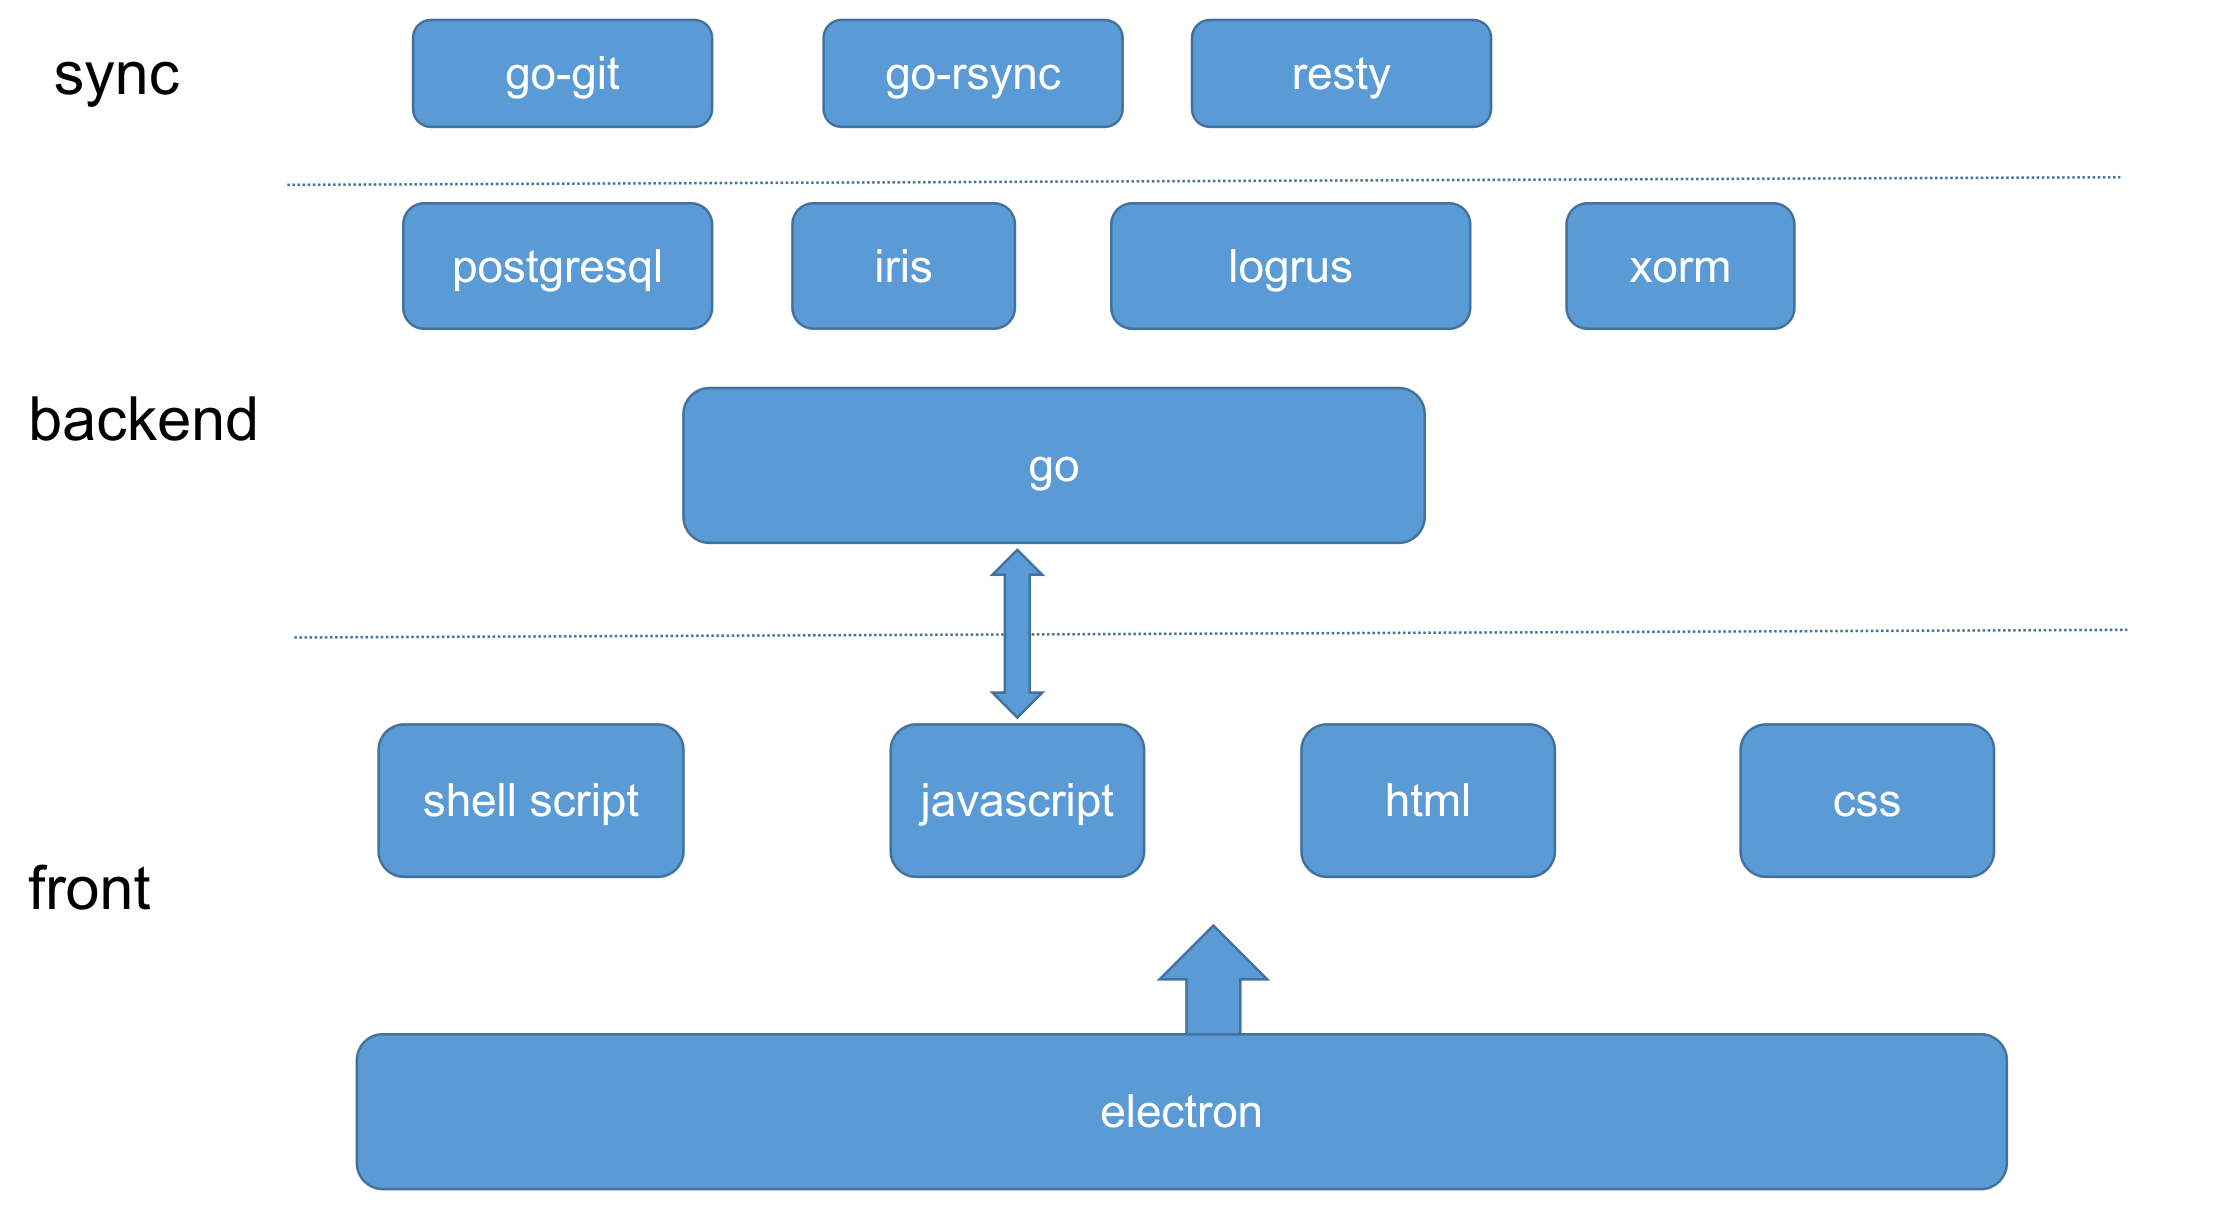
\includegraphics[scale=0.4]{./images/tech.png}
    \caption{技术架构}
	\label{tech}
\end{figure}

软件部署方案,为了保证后端的可移植特性,编写dockerfile将其转换为docker镜像用于部署,同时在运维模块
全部进行虚拟化,使用docker-compose对数据进行监控,最终呈现的运维框架如图\ref{maintain}所示

\begin{figure}[ht]
    \centering
    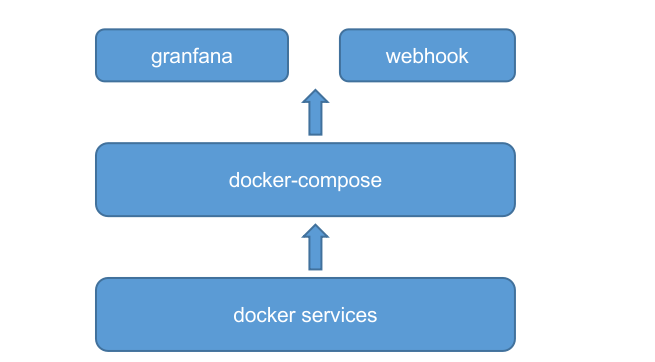
\includegraphics[scale=0.8]{./images/maintain.png}
    \caption{技术架构}
	\label{maintain}
\end{figure}


\subsection{人员管理和项目进度}

项目组人员目前为我一个人,同时HLUG(hust linux user group)的同学提供运维和服务器方面的支持。

在项目进度上通过jira进行进度的管理
\begin{figure}[ht]
    \centering
    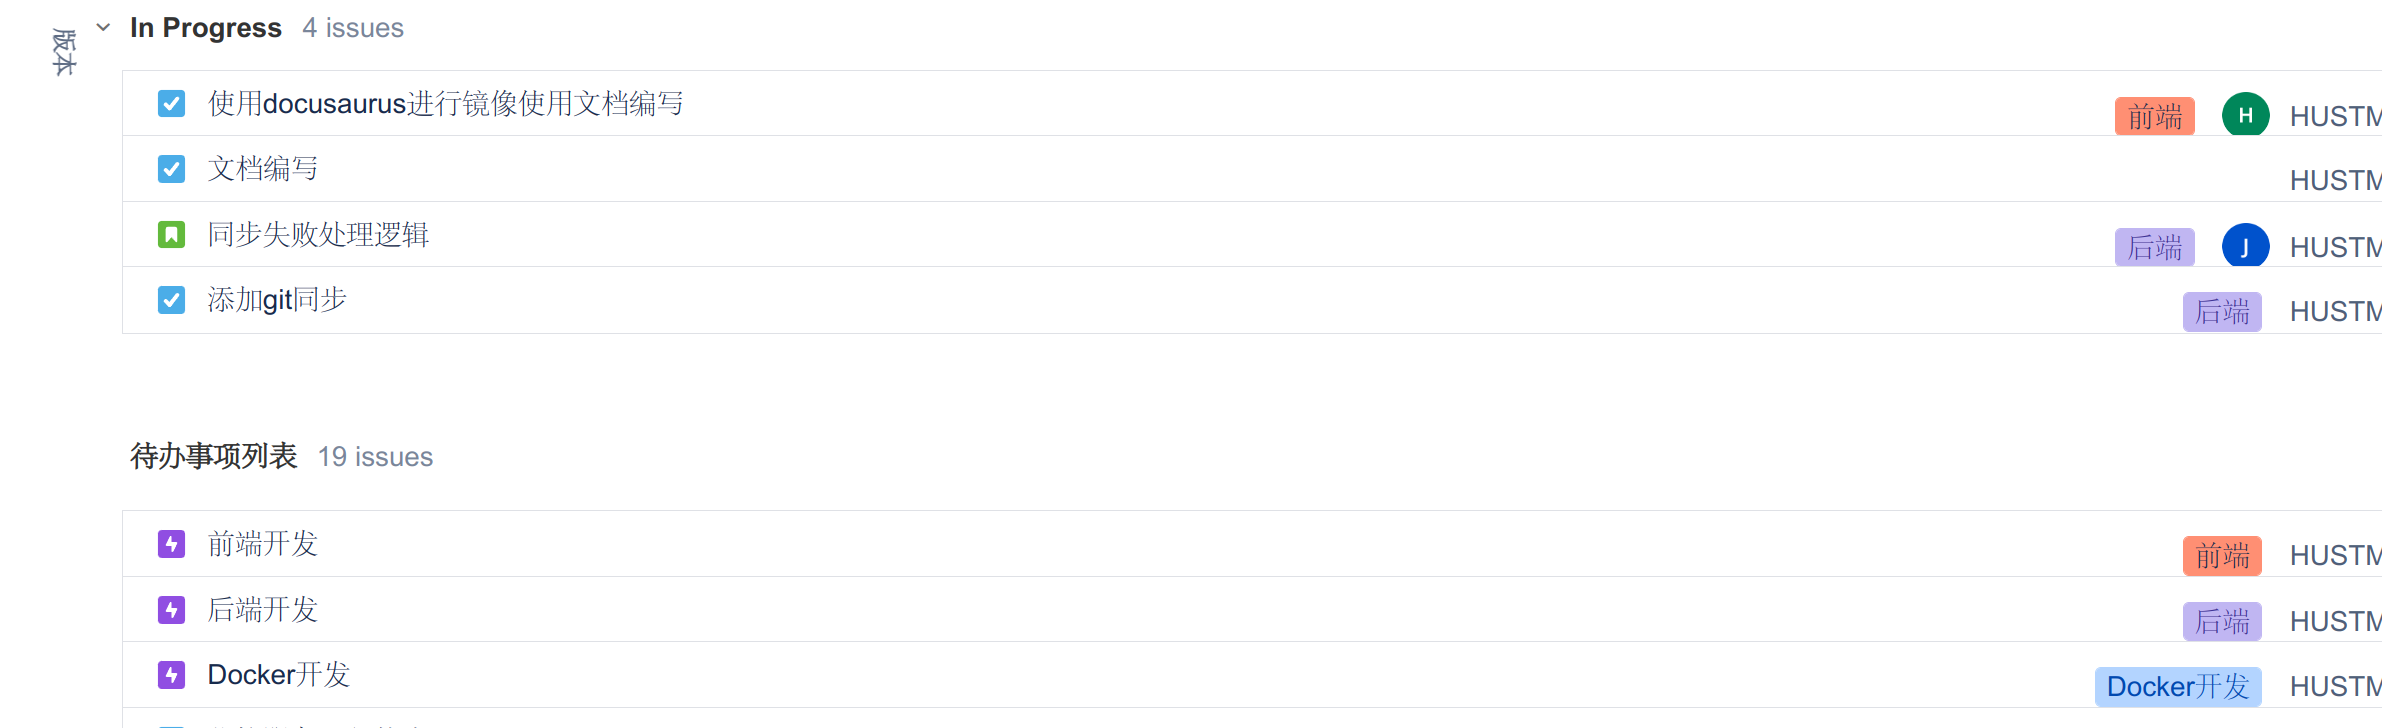
\includegraphics[scale=0.4]{./images/jira.png}
    \caption{进度管理}
	\label{jira}
\end{figure}


\section{需求分析}

\subsection{需求分析概述}
在linux操作系统上,现有的软件商店大多使用Qt进行开发,存在着二次开发难度大以及页面设计缺乏美观和易用性的缺点,整理开发者和用户的需求,
如表1所示。

\begin{table}[!h]
    \setlength{\tabcolsep}{3mm}{}
    \begin{center}
        \begin{tabular}{ccc}        
            \toprule[1pt] 需求端 & 功能\\
            \midrule[1pt]
            用户 & 更加美观人性化的界面\\
            用户 & 可以在不同的机器上同步自己的软件数据,快速部署开发环境\\
            用户 & 可以使用图形化的方式对服务器进行管理\\
            开发者 & 基于本项目进行二次开发\\
            开发者 & 可以发行自己的软件\\
            管理者 & 可以在后台管理软件\\
			管理者 & 进行镜像服务,扩大软件源 \\
            \bottomrule[1pt]
            \end{tabular}
    \end{center}
    \caption{需求分析}
\end{table}

\subsection{UML相关需求分析图}

用户以及开发者的相关需求如图\ref{user}所示

\begin{figure}[!h]
    \centering
    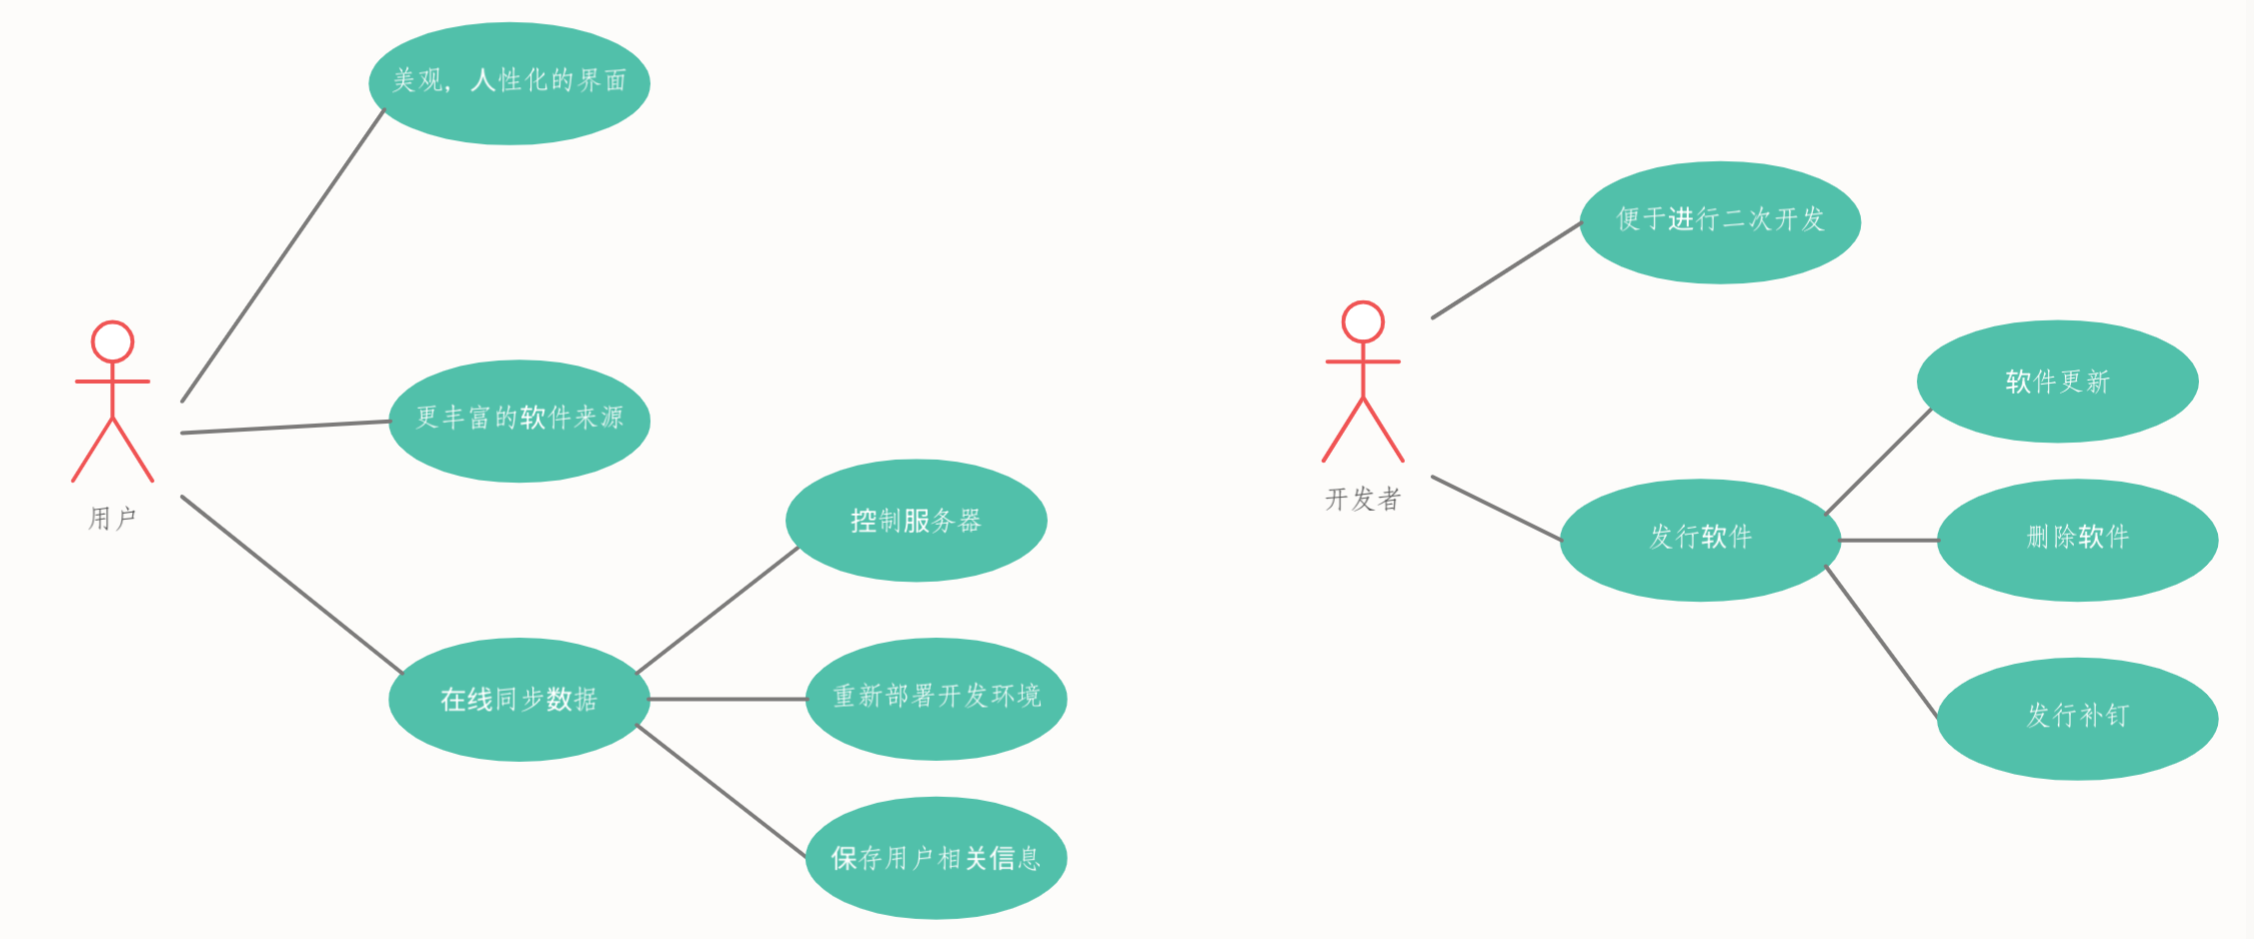
\includegraphics[width=0.8\textwidth]{images/require.png}
    \caption{用户开发者需求}
    \label{user}
\end{figure}

对于管理者的相关需求如图 \ref{manage} 所示
\begin{figure}[!h]
    \centering
    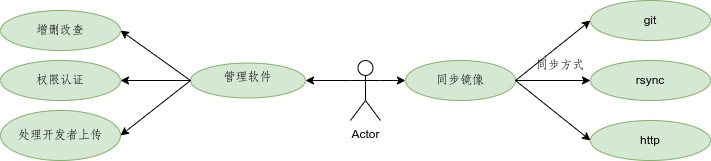
\includegraphics[width=0.8\textwidth]{images/manager.png}
    \caption{管理者需求}
    \label{manage}
\end{figure}

\subsection{原型系统设计}

对于界面的设计我选择使用墨刀进行设计

登录界面设计如图\ref{login}所示, 用户可以在登录界面输入帐号密码进行登录,还可以进行注册,注册界面如图\ref{register}所示
\begin{figure}[ht]
    \caption{登录界面设计}
    \centering
    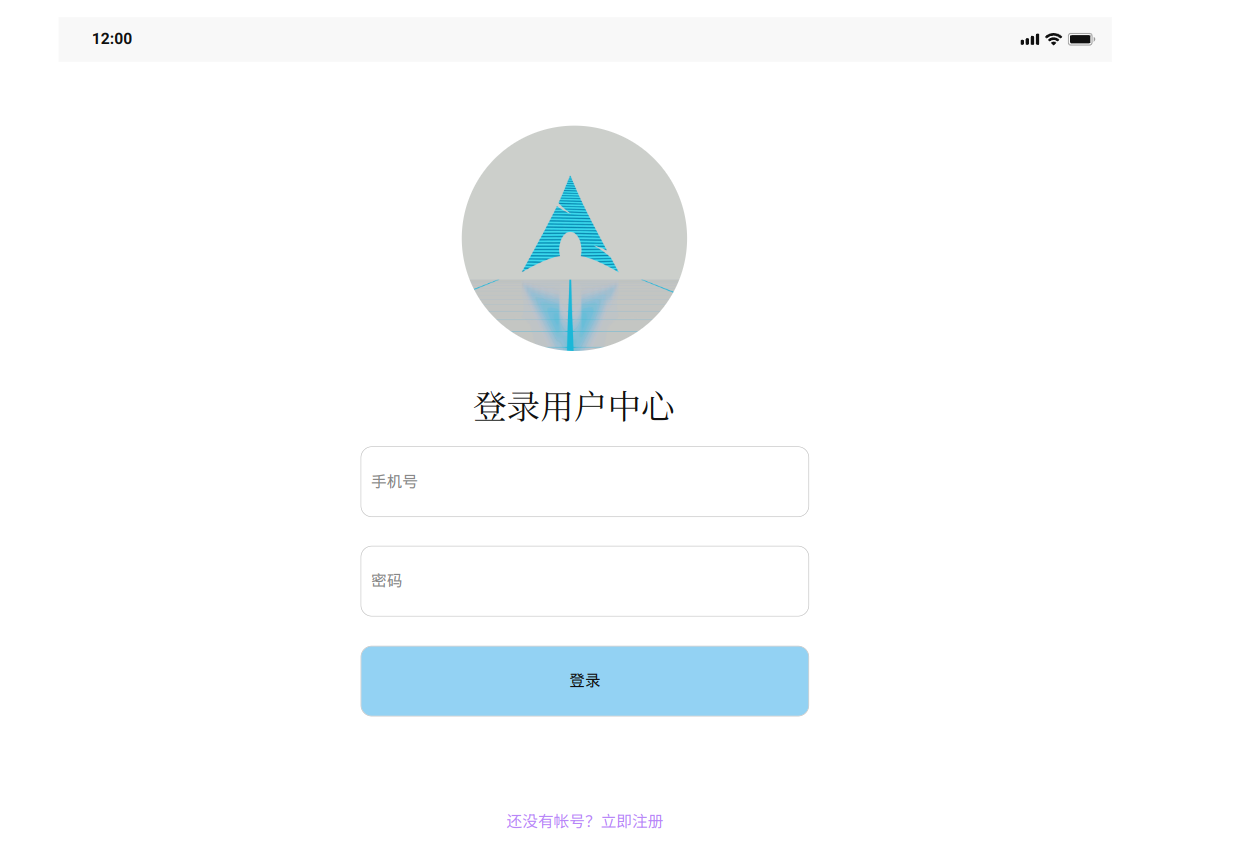
\includegraphics[width=0.7\textwidth]{images/login.png}
    \label{login}
\end{figure}

\begin{figure}[!h]
    \caption{注册页面设计}
    \centering
    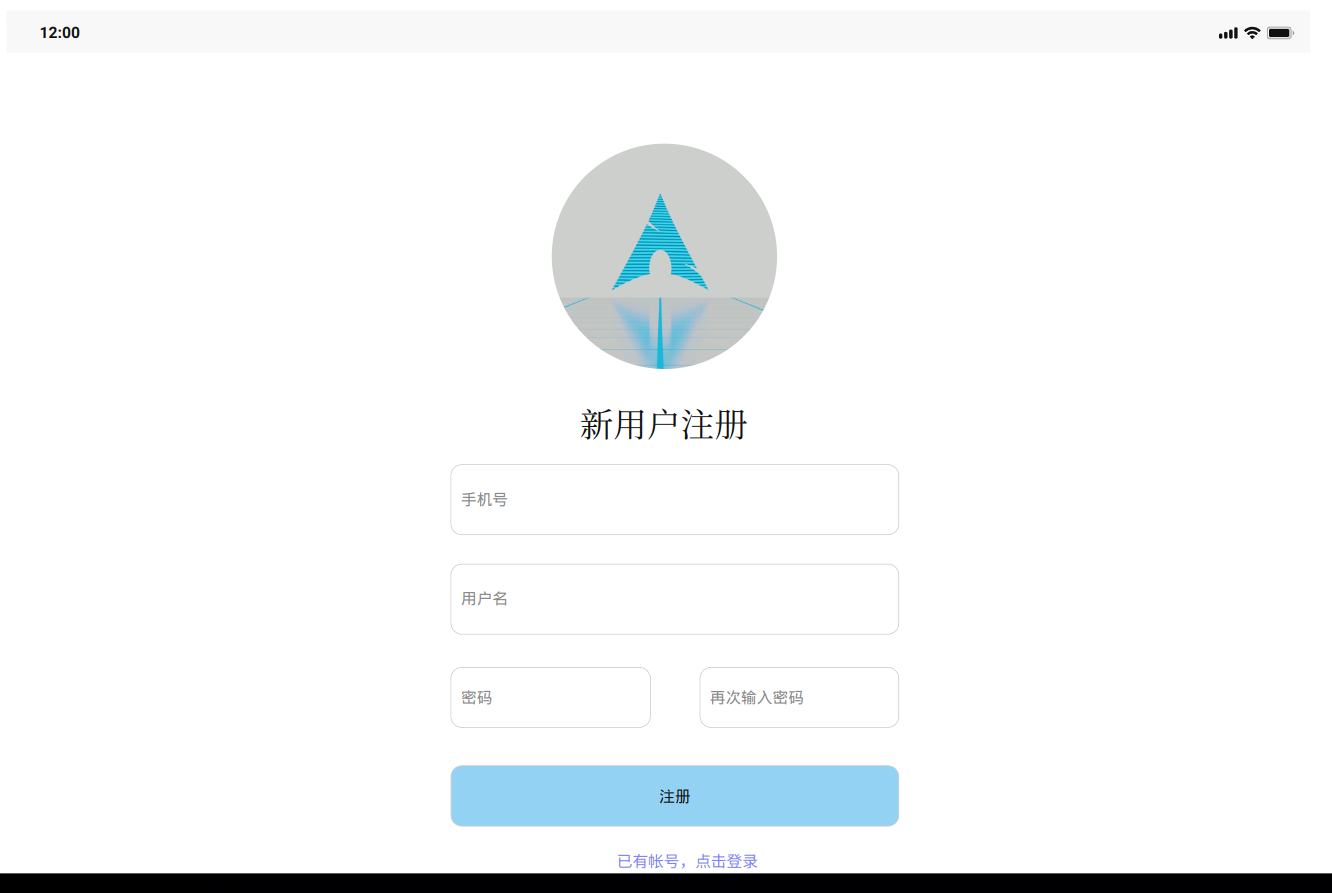
\includegraphics[width=0.7\textwidth]{images/register.png}
    \label{register}
\end{figure}
\newpage
对于我们的主界面,设计如图\ref{main}所示,用户可以通过点击上面的导航栏选择相关的功能。同时在下面的蓝色块中显示一些软件供用户进行下载,点击后进行更加详细的页面。
\begin{figure}[!h]
    \centering
    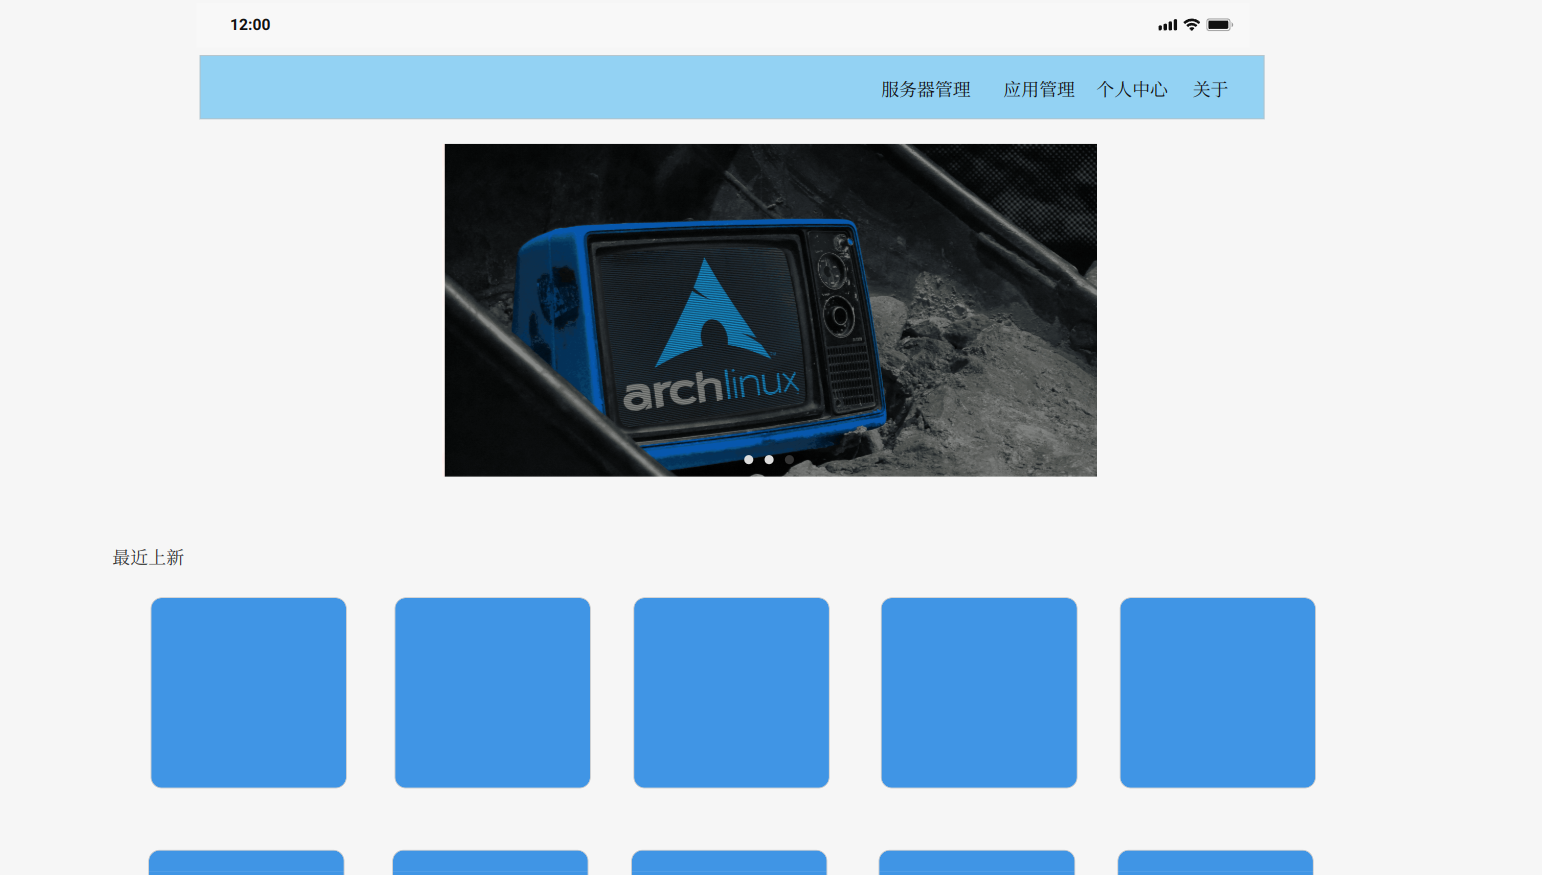
\includegraphics[width=0.8\textwidth]{images/main.png}
    \caption{主界面设计}
    \label{main}
\end{figure}

点击上面的导航栏进入应用中心, 应用中心的默认界面是显示我们的主机上的软件,后续应该支持更新和删除两个功能,通过上面的导航栏可以进入下载界面。
\begin{figure}[!h]
    \centering
    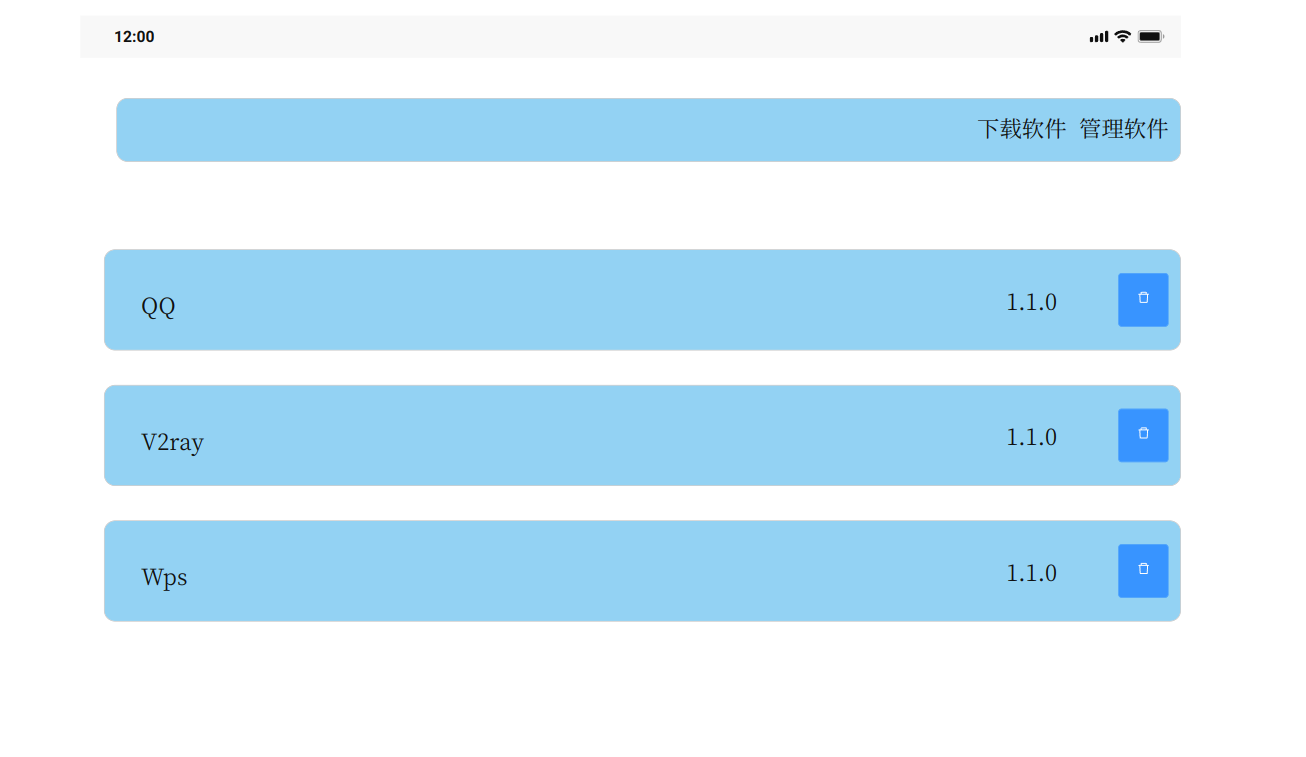
\includegraphics[width=0.8\textwidth]{./images/app.png}
    \caption{应用中心设计}
\end{figure}

\newpage
下载页面的设计如图\ref{download}所示,用户在输入框中输入软件名称,点击搜索按钮可以在下面的列表中
显示软件列表,点击安装按钮对软件进行安装。
\begin{figure}[!h]
    \centering
    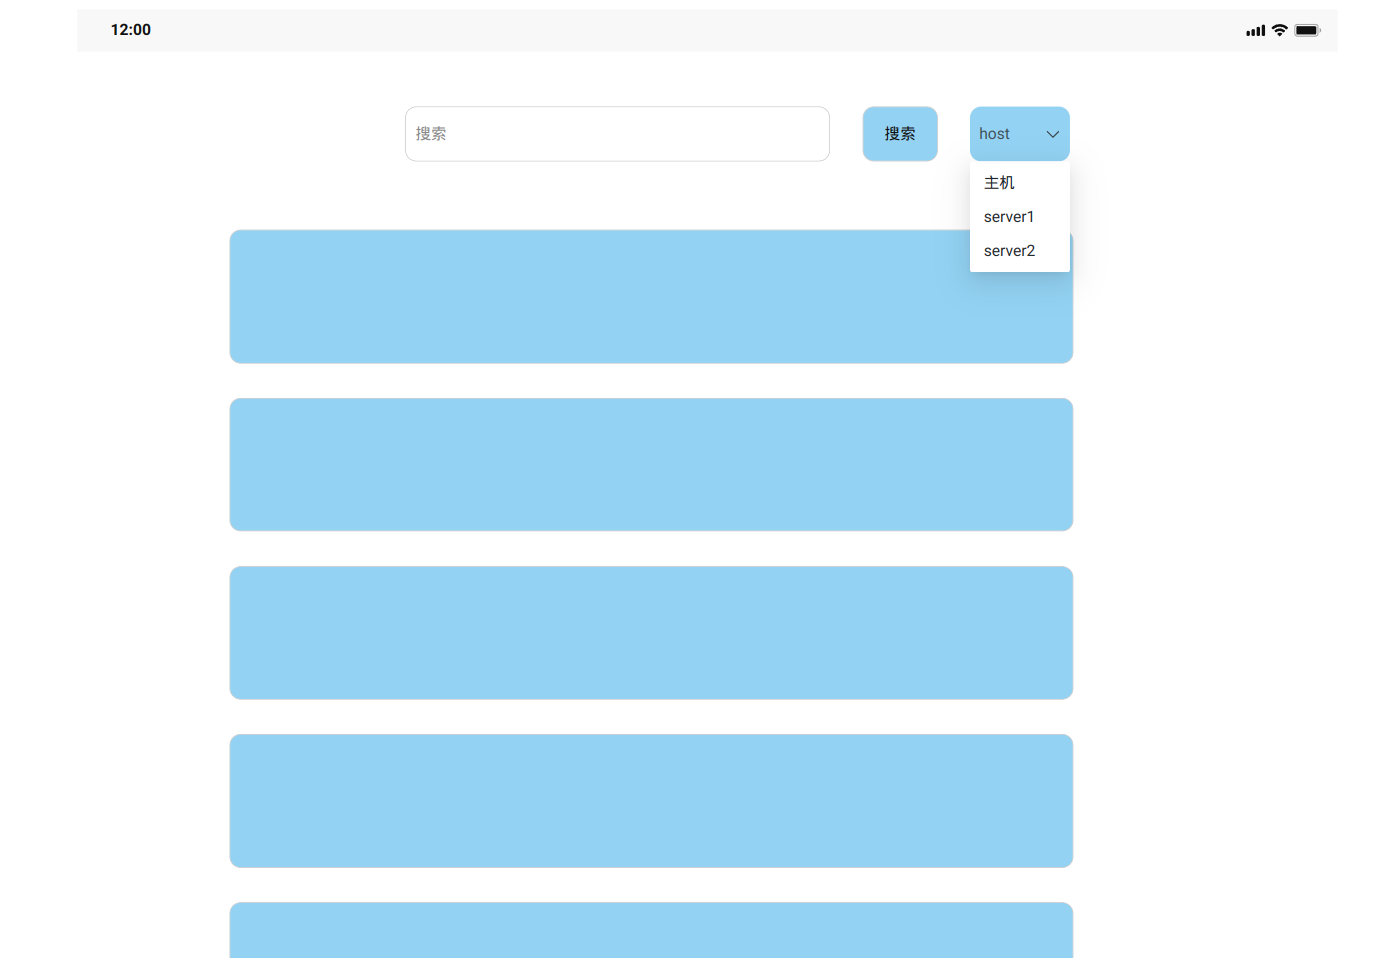
\includegraphics[width=0.8\textwidth]{./images/download.png}
    \caption{下载界面设计}
    \label{download}
\end{figure}

\newpage
在开发者方向,设计的页面如图8所示,开发者可以管理自己发布的软件和发布新软件。
\begin{figure}[!h]
    \caption{开发者页面}
    \centering
    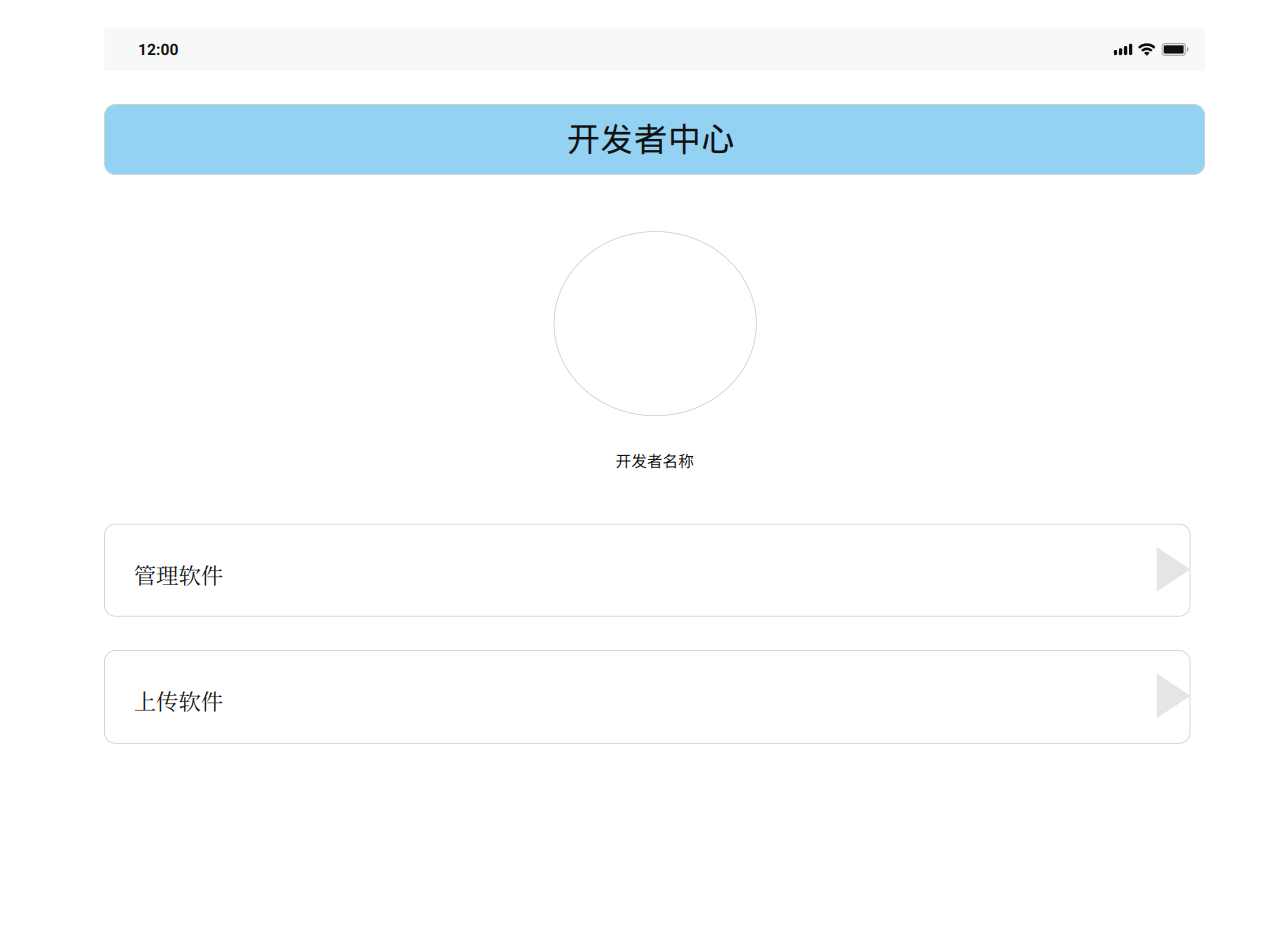
\includegraphics[width=0.8\textwidth]{./images/develop.png}
	\label{develop}
\end{figure}

\newpage
\section{概要设计和详细设计}
\subsection{系统结构}
整个软件商店的项目,可以分解为客户端,服务器端和运维三个部分,客户端和服务端两个模块之间通过GET/POST的方式的进行通信,
client调用server端提供的api完成部分功能。

客户端的工作在于进行登录,并向服务器上传软件包,软件信息,用户信息等数据,也可以向服务器进行查询请求,同时可以调用系统中的包管理器
进行系统包的管理。

服务器端的工作在于处理客户端的请求,对于不同的功能提供了不同的api供client进行调用。

对于运维的部分,每次push的时候将会触发CI/CD,进行自动化的部署
最终实现的系统结构如图\ref{struct}所示
\begin{figure}[!h]
    \caption{系统结构}
    \centering
    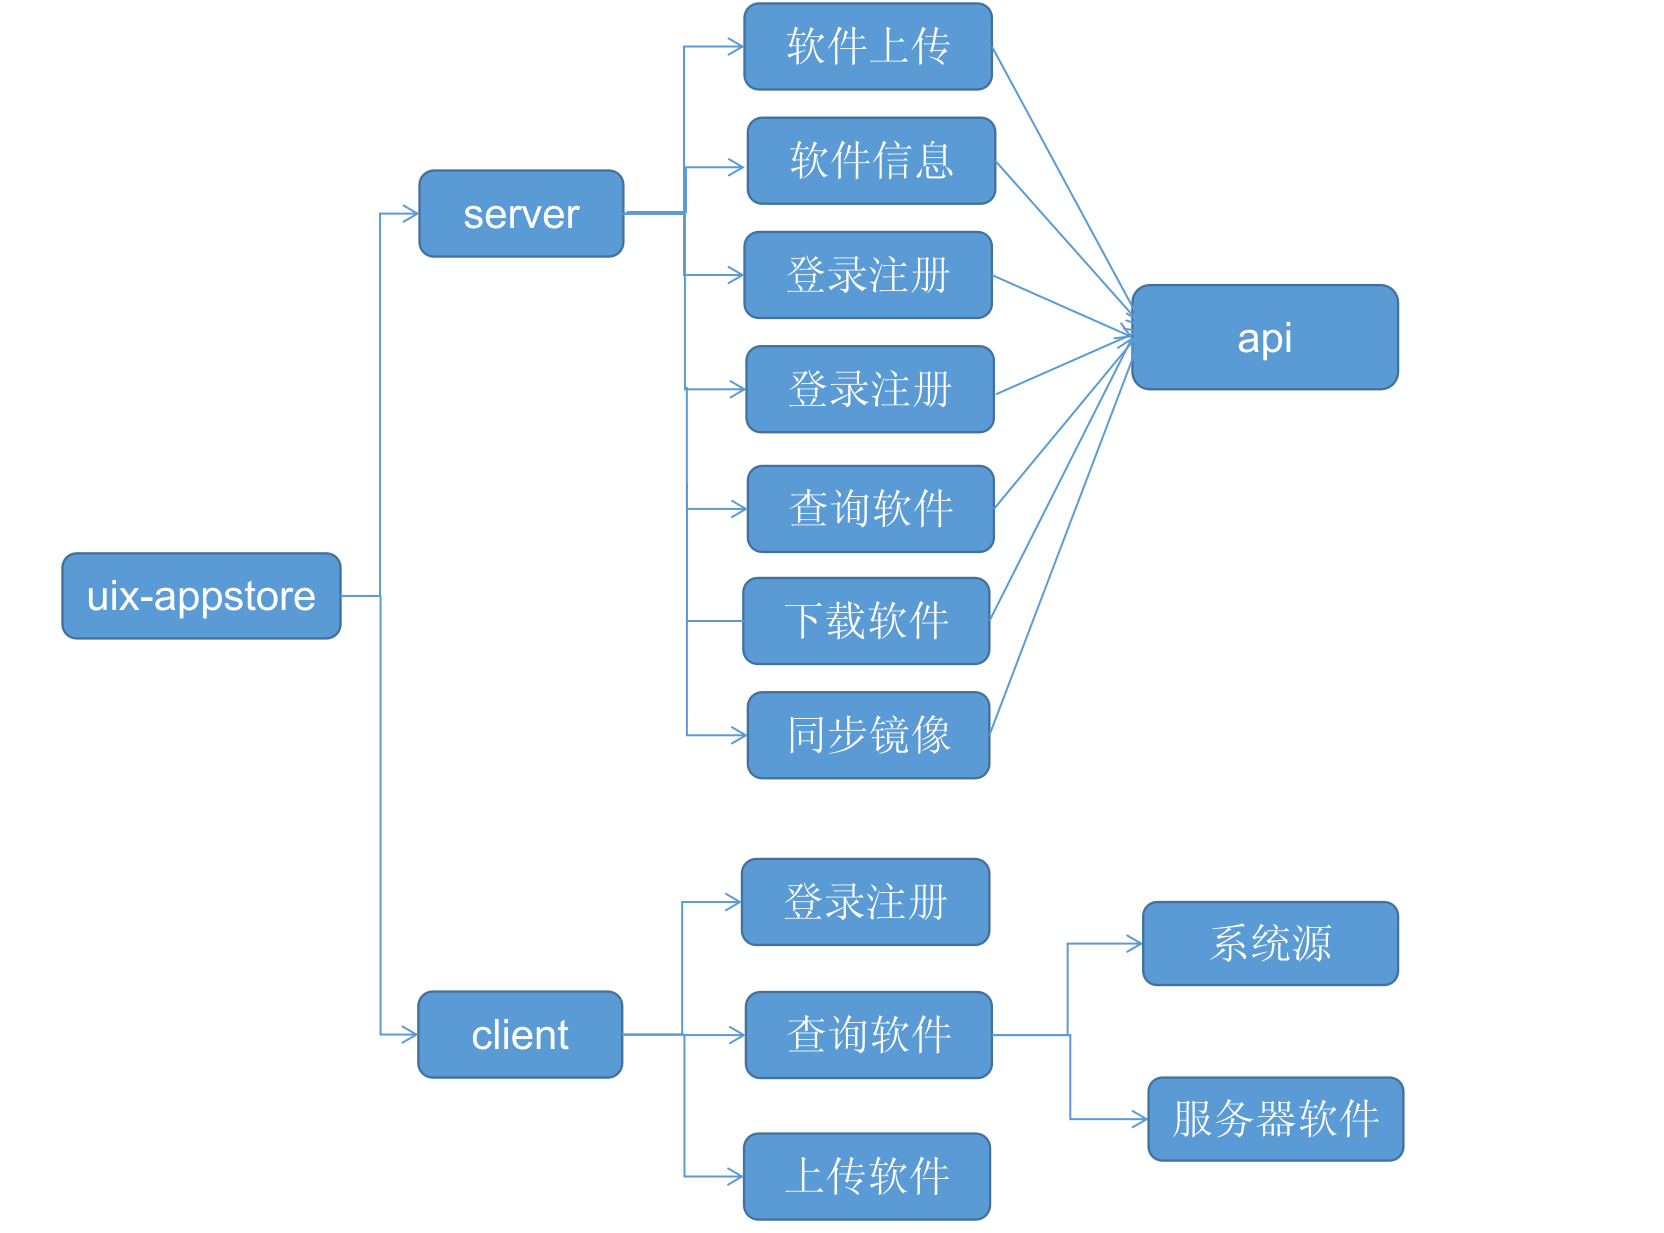
\includegraphics[width=0.8\textwidth]{./images/struct.png}
    \label{struct}
\end{figure}
\newpage

持续集成部署模块如图\ref{CID}所示
\begin{figure}[!h]
    \caption{持续集成部署}
    \centering
    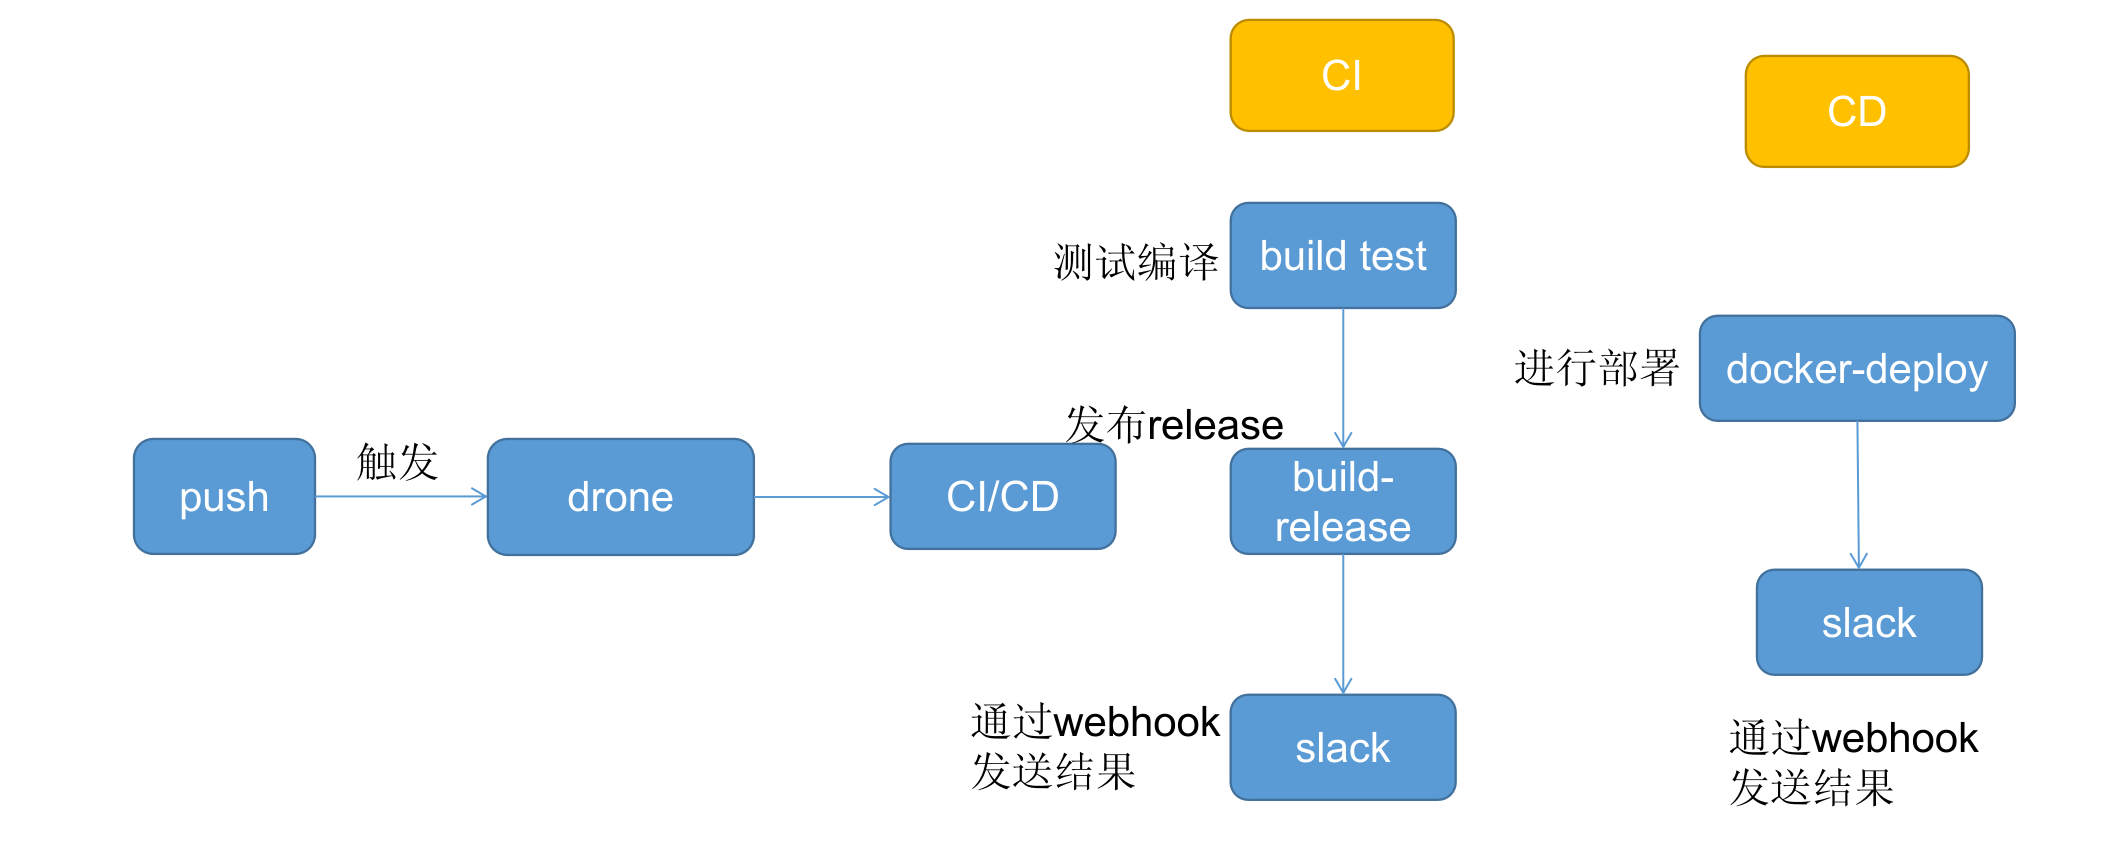
\includegraphics[width=1\textwidth]{./images/CID.png}
    \label{CID}
\end{figure}

\subsubsection{功能说明}

客户端的功能说明如表3-1 所示

\begin{table}[!h]
    \setlength{\tabcolsep}{6mm}{}
    \begin{center}
		\caption{需求分析}
        \begin{tabular}{ccc}        
            \toprule[1pt] 需求端 & 功能\\
            \midrule[1pt]
            用户注册 & 通过用户名,手机号,密码等数据进行注册\\
			用户登录 & 通过手机号和密码进行登录 \\
			软件查询 &  \begin{tabular}[c]{@{}l@{}}
				软件查询分为两种方式,一种是在本地进行查询,\\
				一种是向远程服务器发起请求进行查询,本地查询时\\
				调用本地的包管理器进行软件包的查询
				将查询结果\\解析为json文件后呈现在页面上。\\
				\end{tabular}\\
			软件包传输 & \begin{tabular}[c]{@{}l@{}}
				对开发者的身份进行验证后将其软件包传输到远端
				\end{tabular}\\
				软件下载& \begin{tabular}[c]{@{}l@{}}
					软件下载统一分为两种,一种是本地使用包管理器进行下载,\\
					一种是远程下载,向服务器发起请求下载所需的软件。\\
				\end{tabular}\\
				软件管理& \begin{tabular}[c]{@{}l@{}}
					对本地的软件进行管理,进行删除等操作
				\end{tabular}\\
            \bottomrule[1pt]
            \end{tabular}
    \end{center}
	\label{client1}
\end{table}

\subsection{接口设计}

\paragraph*{服务端客户端接口:}

客户端通过向服务器端发起HTTP请求,服务端进行响应,将请求的数据以json的形式存储在报文中,得到的接口设计如表\ref{table:server_api}所示

\begin{table}[h]
    \begin{center}
        \begin{tabular}{ccc}
            \toprule[1pt] 
            接口名称 & 传递参数 & 返回值\\ 
            \midrule[1pt]
            软件上传 &文件路径& null\\
            登录&密码,手机号& 登录成功返回一个ID,否则返回错误信息\\
            注册&用户名,手机号,密码&注册成功返回一个ID,否则返回错误信息\\
            软件信息上传&\begin{tabular}[c]{@{}l@{}}
				软件名,二进制包名,\\版本号,上传时间,开发者\\
			\end{tabular} &null\\
            软件搜索& 软件名& 查询到的相关软件信息数组\\
            软件下载& 软件名& 二进制软件包\\
			软件源同步& 镜像信息& 同步情况\\
            获取软件源信息 &null& 所有软件源信息\\
            \bottomrule[1pt]
        \end{tabular}
        \caption{服务器端接口}
        \label{table:server_api}
    \end{center}
\end{table}

\paragraph*{客户端模块之间的接口设计:}
客户端的接口主要在于界面到js,以及js和底层脚本的交互
\begin{table}[h]
    \begin{center}
        \begin{tabular}{ccc}
            \toprule[1pt] 
            接口名称 & 传递参数 & 返回值\\ 
            \midrule[1pt]
            包管理器软件查询 &查询的软件名称& 包含版本号,软件名,来源\\
            此项目源软件查询 & 查询的软件包名称& 所有符合条件的软件包的详细信息\\
            登录&密码,手机号& 登录成功进入主页面\\
            注册&用户名,手机号,密码&注册成功进入主页面\\
            下载软件 & 点击下载按钮 & 下载成功显示已下载 \\
            删除软件 & 点击删除按钮 & 成功后将从软件目录中消失\\
            上传软件& 通过页面选择软件包 & null\\
            上传软件信息 & 输入软件名,二进制包名,版本号& null\\
            \bottomrule[1pt]
        \end{tabular}
        \caption{客户端接口}
        \label{table:server_api}
    \end{center}
\end{table}

\subsection{类图}

\subsubsection{数据库类图设计}

在数据库方面使用ORM技术来进行操作,orm技术可以将关系型数据库中的数据映射到具体的对象中,使用面向对象的方式对数据库进行操作。

\begin{figure}[!h]
    \centering
    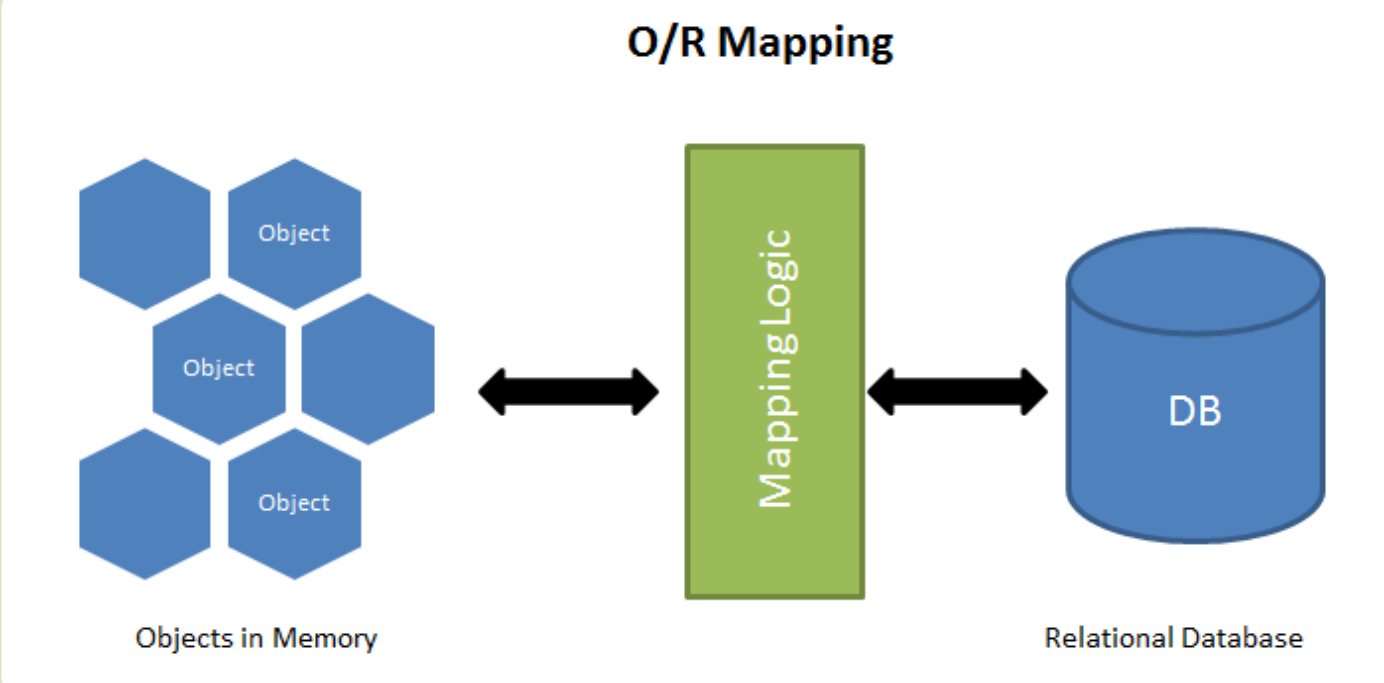
\includegraphics[width=0.8\textwidth]{./images/orm.png}
    \caption{orm模型}
    \label{database}
\end{figure}

具体到我们的项目中则是如图\ref{xdatabase}所示
\begin{figure}[!h]
    \centering
    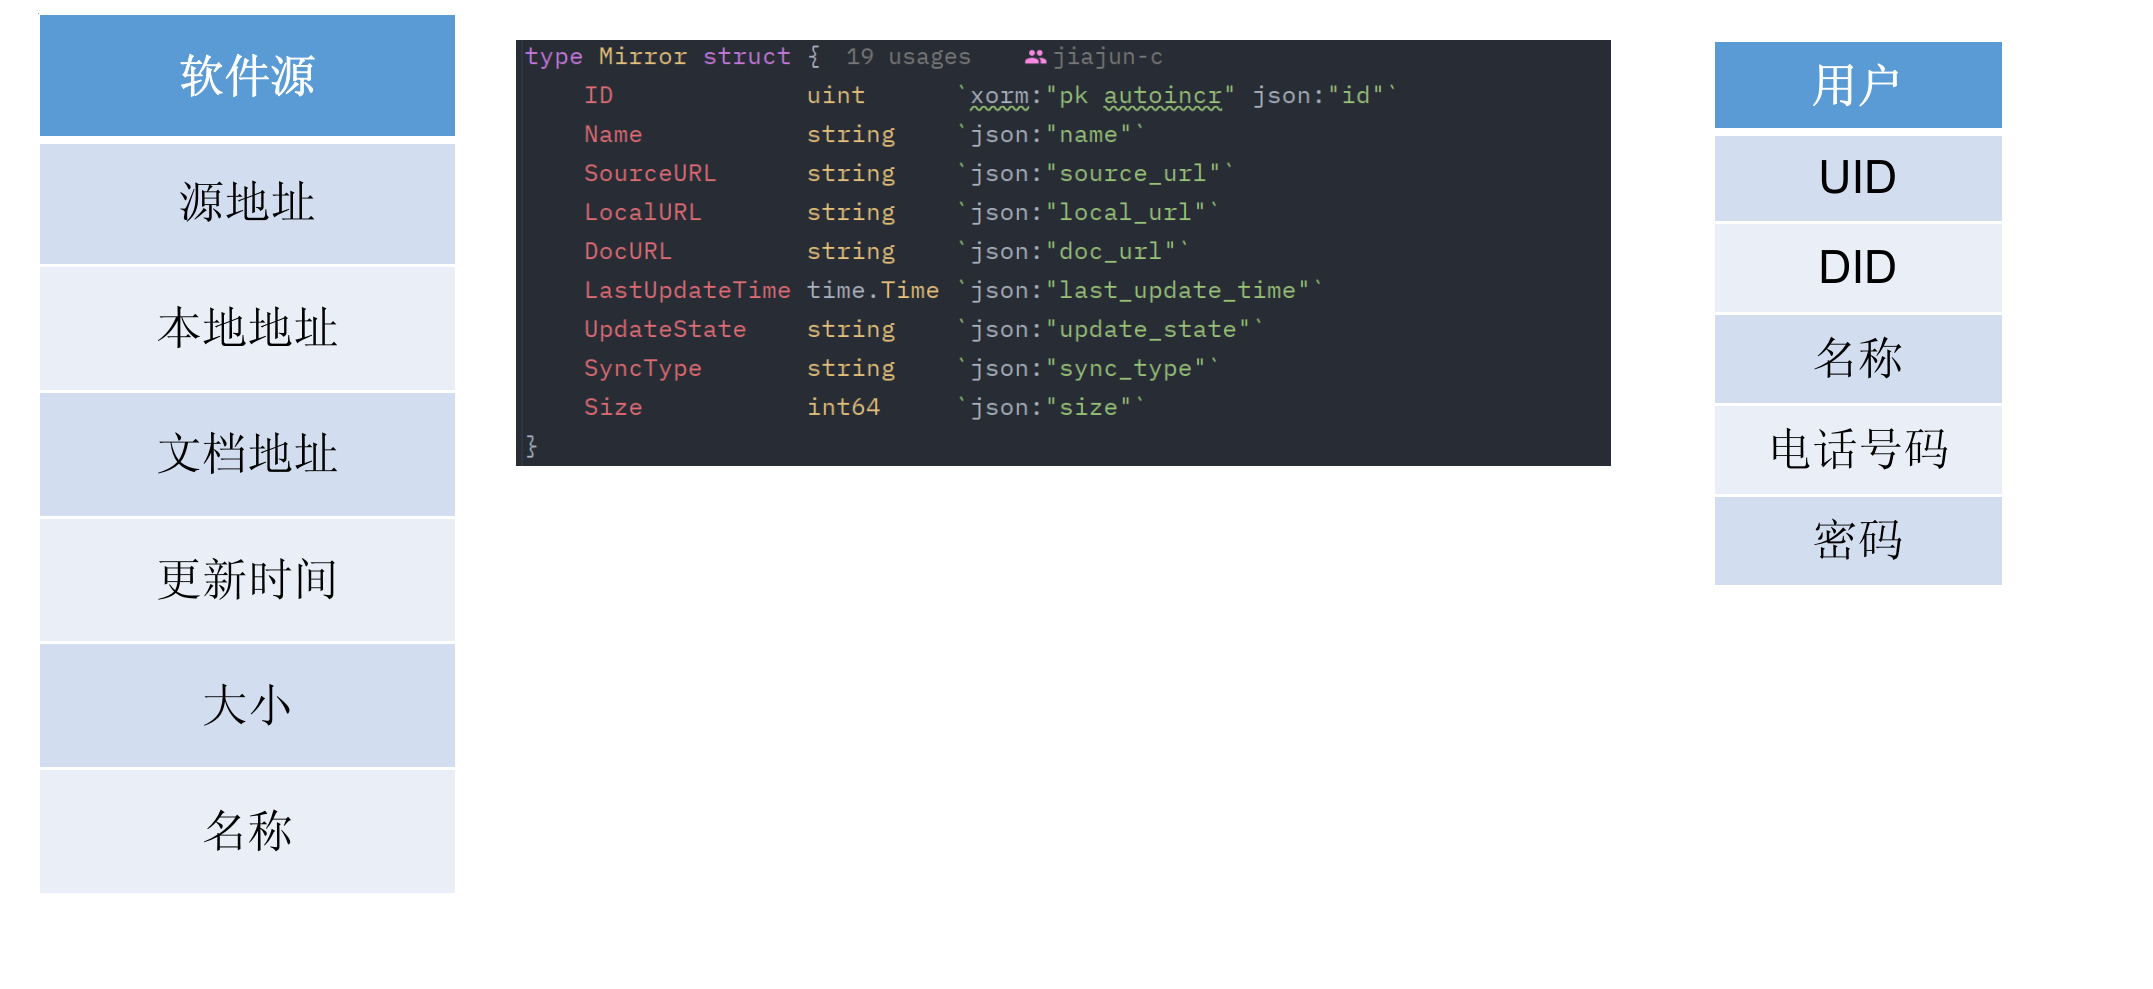
\includegraphics[width=1.0\textwidth]{./images/xorm.png}
    \caption{数据库类}
    \label{xdatabase}
\end{figure}
\newpage
对于开发者和软件部分的则如下所示
\begin{figure}[!h]
    \centering
    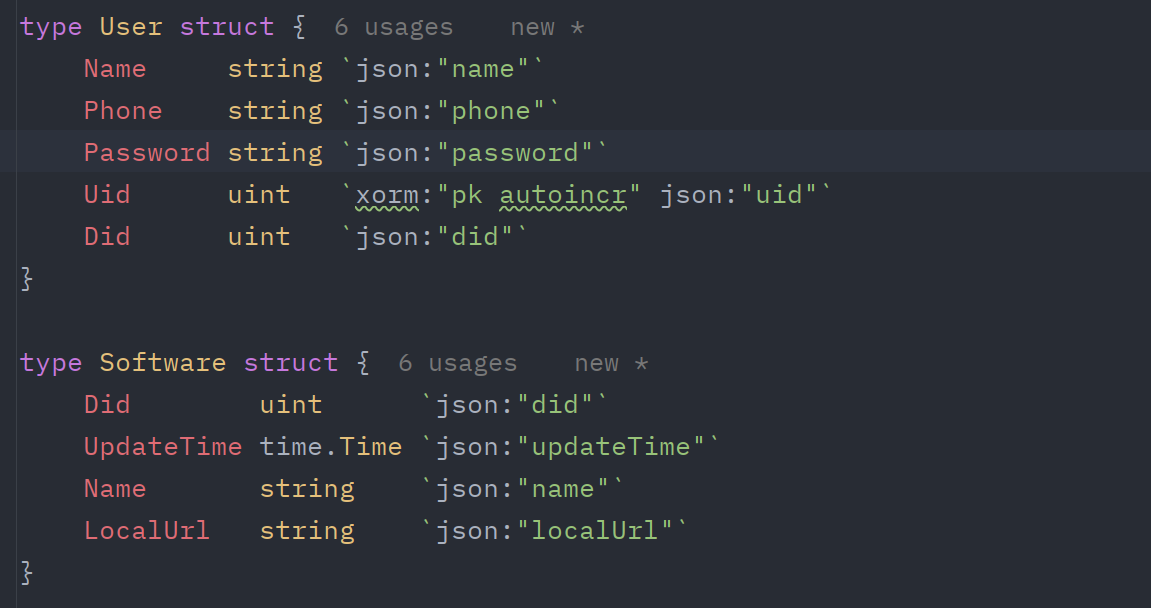
\includegraphics[width=1.0\textwidth]{./images/dev.png}
    \caption{软件以及开发者}
    \label{Software}
\end{figure}


\subsection{关键数据结构定义}
关键数据结构的定义主要是在后端模块,使用golang的接口和结构体定义了一系列的关键数据结构,
在从上游的软件源进行同步时,上游一般提供三种方式进行同步,git, http和rsync,由于他们的功能相同,所以需要
实现相同的接口。
\begin{figure}[!h]
    \centering
    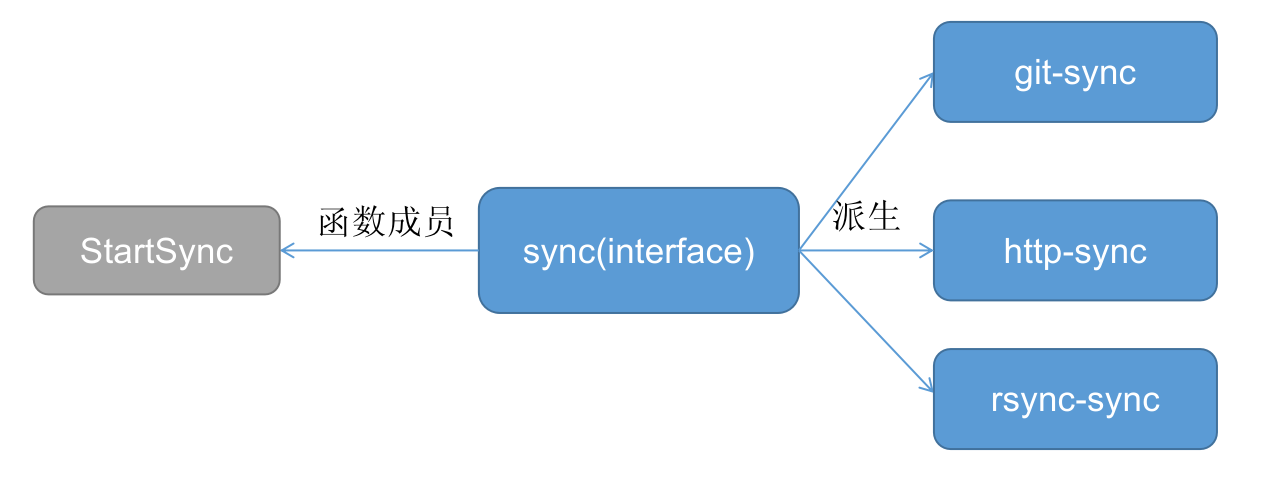
\includegraphics[width=1.0\textwidth]{./images/sync.png}
    \caption{软件源同步设计}
    \label{sync}
\end{figure}

\subsection{关键算法实现}
\subsubsection{客户端部分算法实现}

在进入客户端的时候,如果用户之前已经登录,那么会在本地留下记录,用户可以直接进入客户端,否则进入登录注册的
界面。
\begin{figure}[!h]
    \centering
    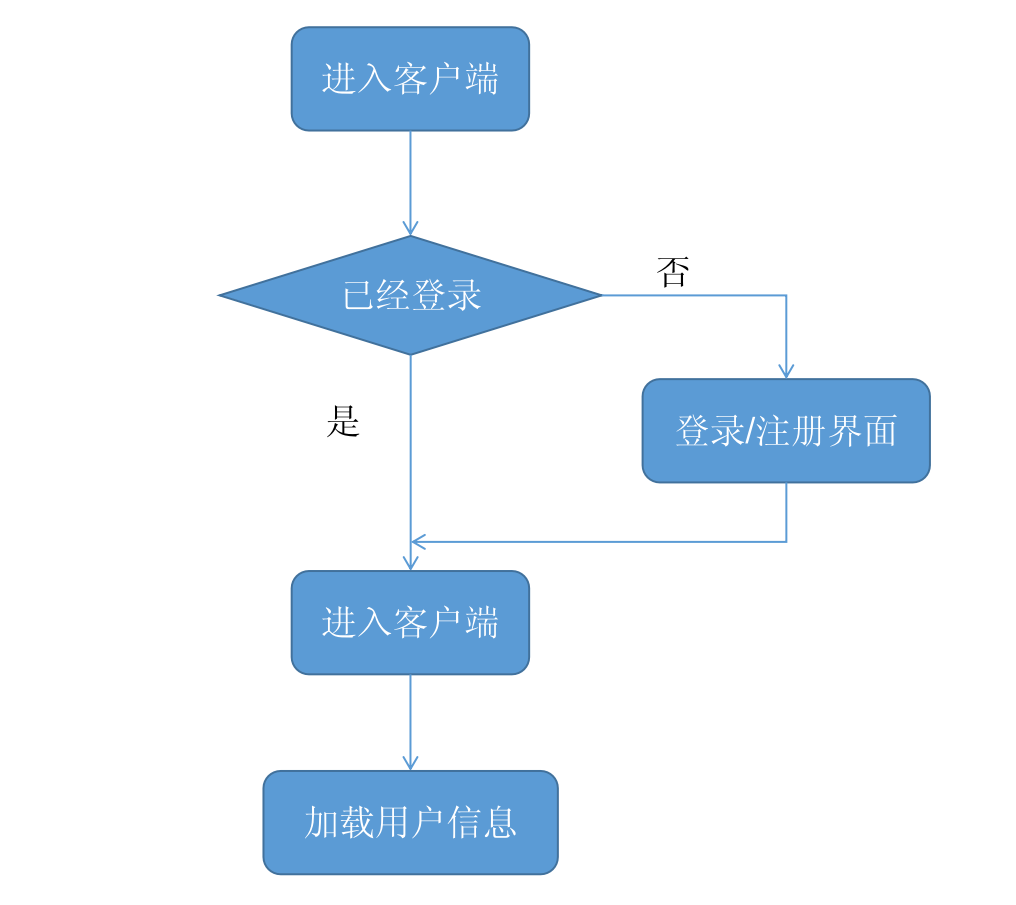
\includegraphics[width=0.5\textwidth]{./images/log_al.png}
    \caption{登录算法}
    \label{login_al}
\end{figure}

在进入客户端后,可以进行搜索的工作,主要是通过包管理器进行搜索安装,使用python进行结构处理。
目前只支持archlinux进行使用

\begin{figure}[!h]
    \centering
    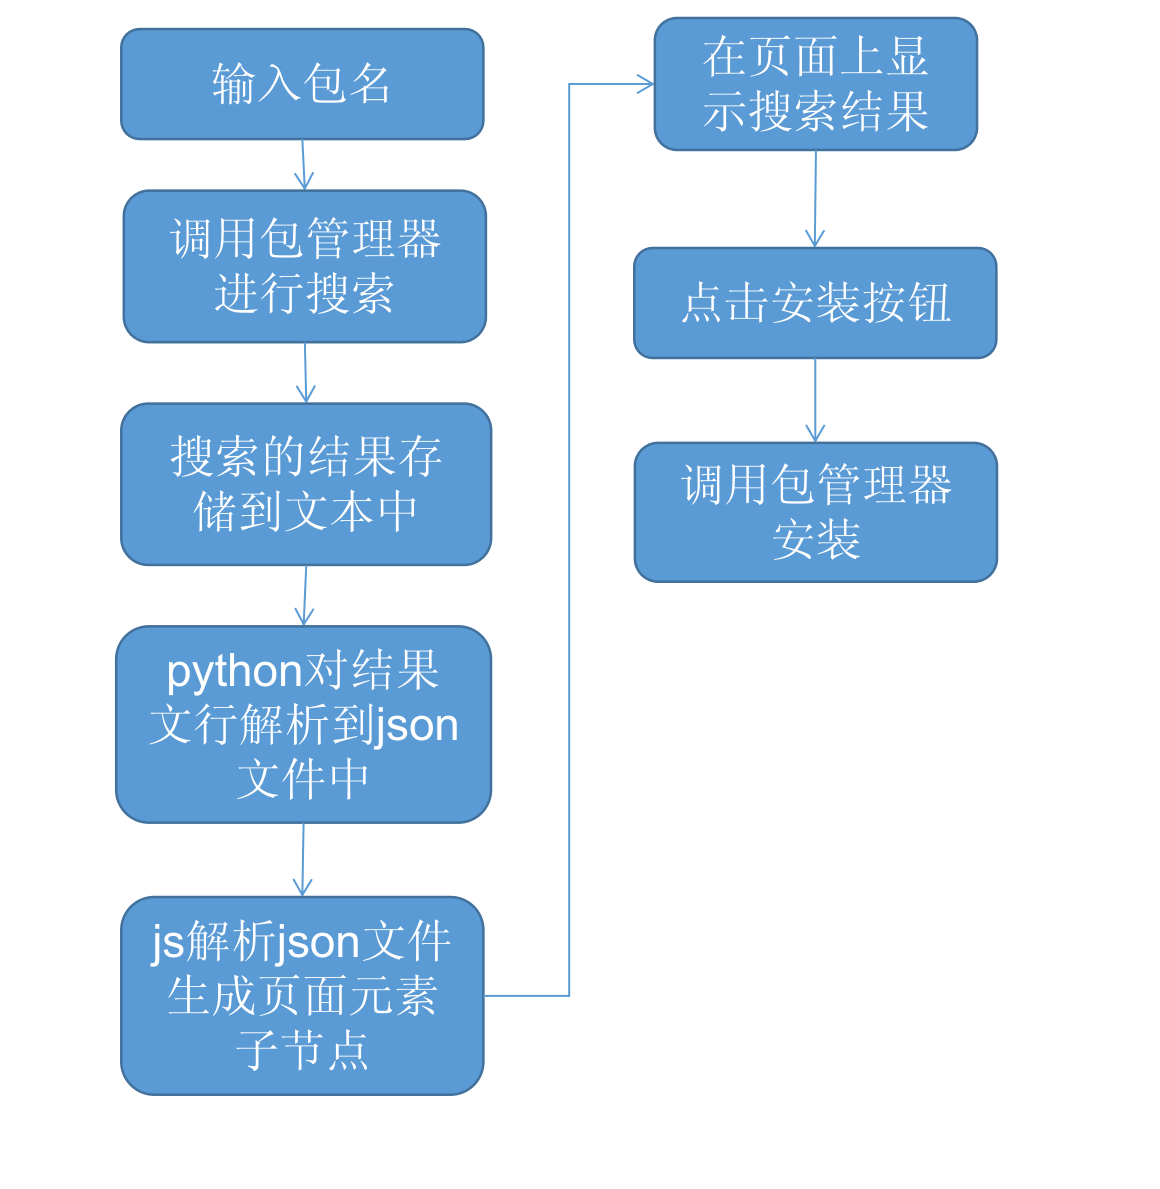
\includegraphics[width=0.5\textwidth]{./images/search.png}
    \caption{搜索算法}
    \label{search}
\end{figure}

此外还可以进行本地包的管理。
\newpage
\begin{figure}[!h]
    \centering
    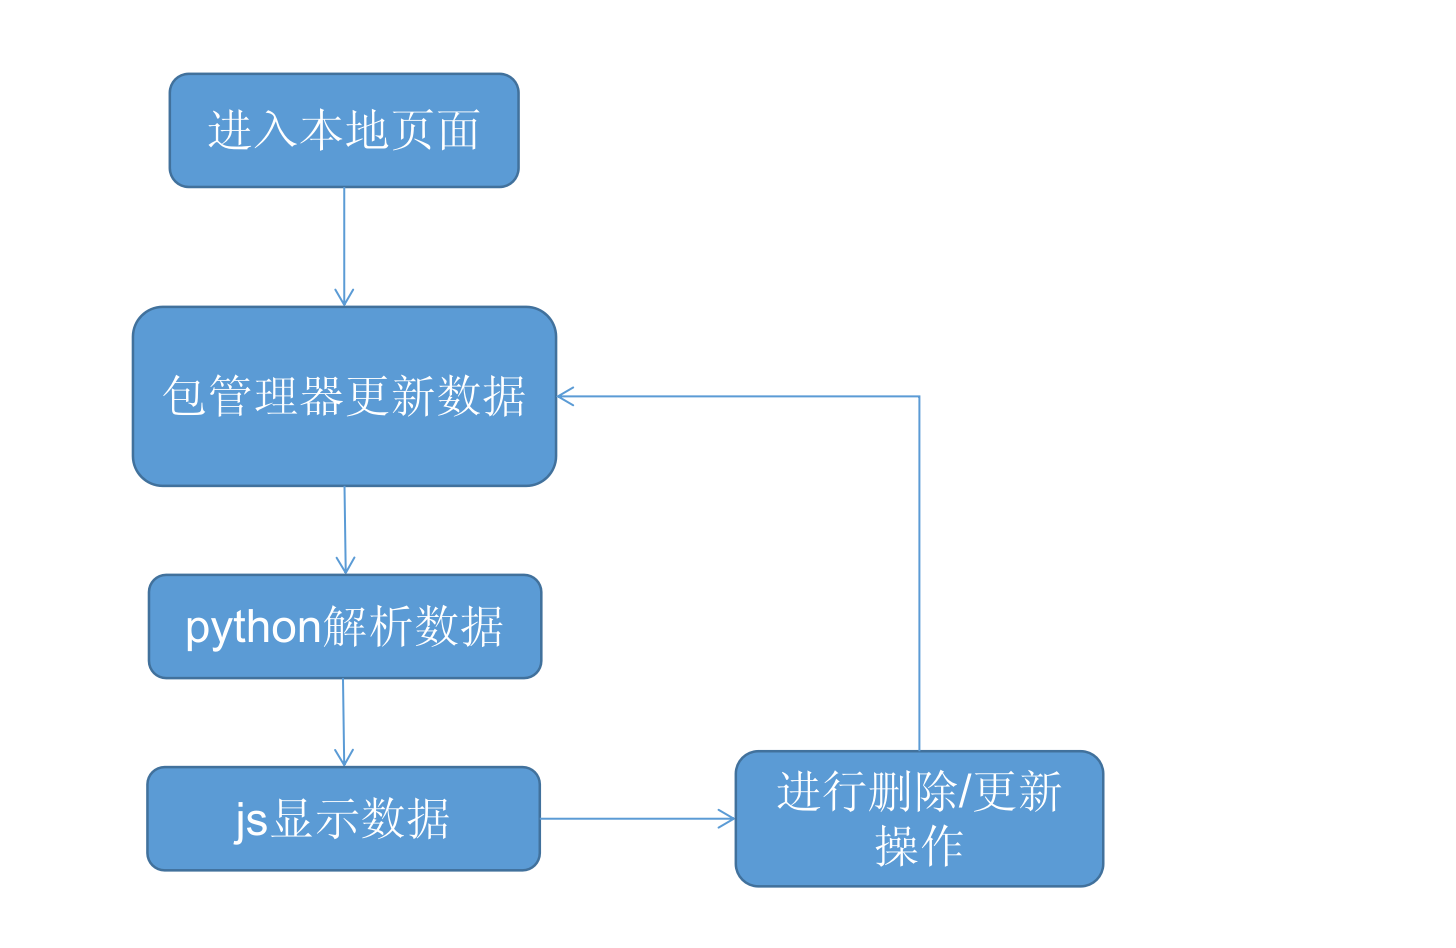
\includegraphics[width=0.7\textwidth]{./images/del.png}
    \caption{本地包管理}
    \label{del}
\end{figure}

\subsubsection{后端算法实现}
在后端中对于一个业务逻辑的处理分为多个阶段,对于数据库方面的算法实现如图\ref{curd}所示
对于用户数据,软件数据,镜像软件源的信息管理是通过xorm进行实现,然后为上层调用提供接口

\begin{figure}[!h]
    \centering
    
\includegraphics[width=0.9\textwidth]{./images/crud.png}
    \caption{数据管理逻辑}
    \label{curd}
\end{figure}

对于后端软件源同步的逻辑如图所示

\begin{figure}[!h]
    \centering
    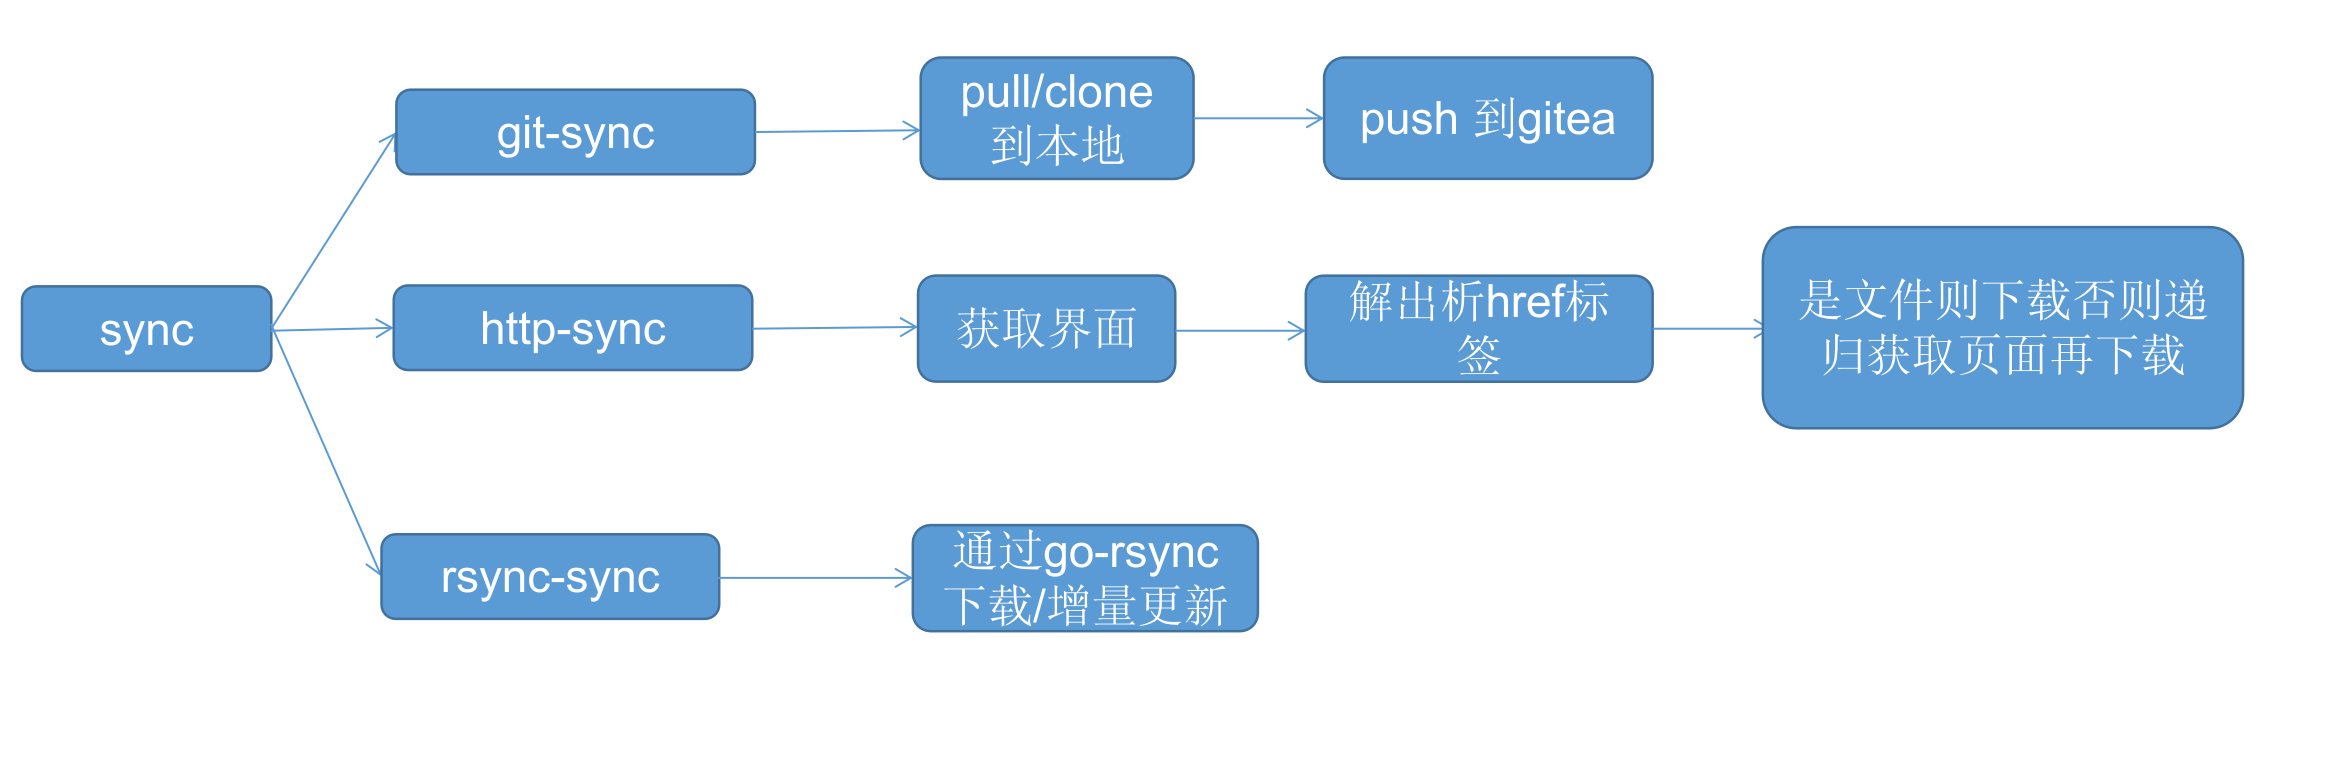
\includegraphics[width=0.9\textwidth]{./images/sync_s.png}
    \caption{数据管理逻辑}
    \label{sync_s}
\end{figure}

后端软件上传逻辑如图\ref{soft}所示
\begin{figure}[!h]
    \centering
    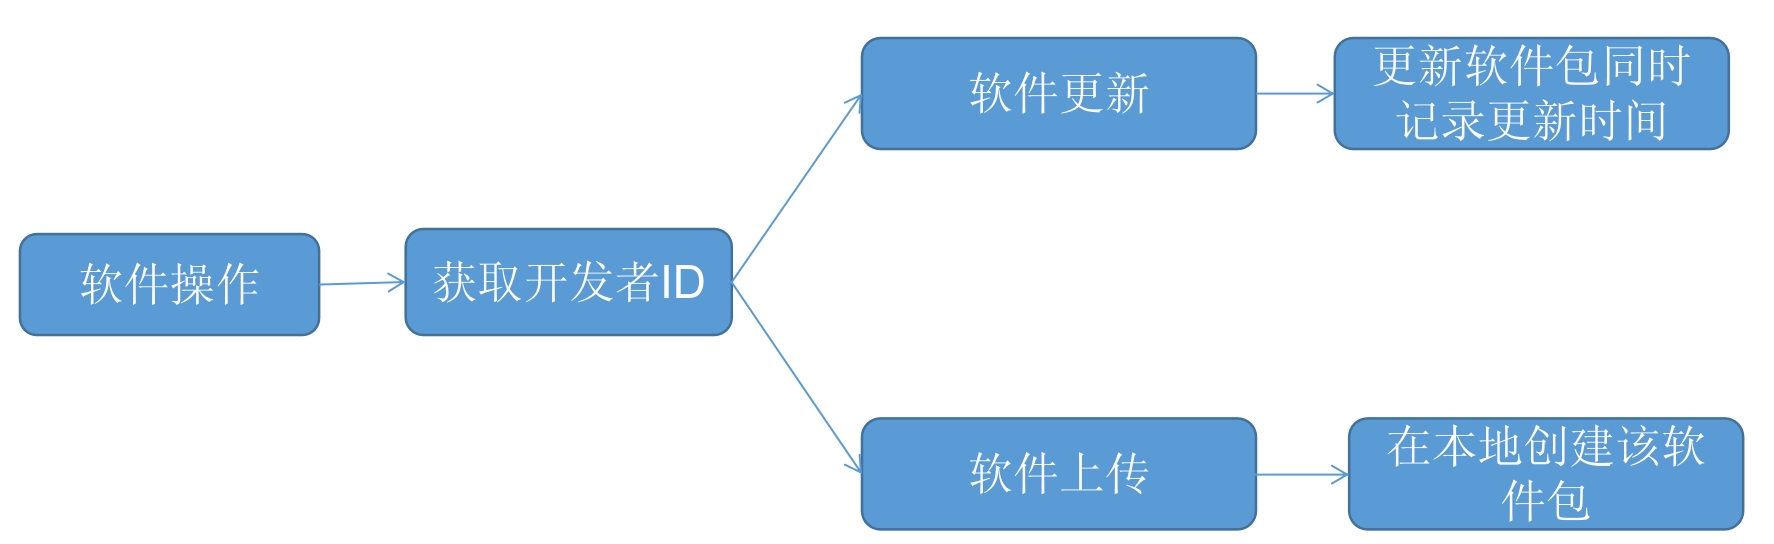
\includegraphics[width=0.9\textwidth]{./images/soft.png}
    \caption{软件上传处理}
    \label{soft}
\end{figure}

\subsection{数据管理说明}

一部分数据存放在客户本地,比如本地的软件数据等,服务端的数据存放在学校的一台服务器上,
在该服务器上运行着虚拟化的程序,同步通过目录映射进行绑定。

对于用户信息,软件信息等数据存放在服务器中的postgresql容器中,通过端口映射的方式对其进行访问。

\section{实现与测试}

\subsection{实现环境与代码管理}

项目分为前端和后端,前端的实现环境是本地,操作系统为archlinux,使用npm进行编译。
后端的实现环境则是在远程的一台gentoo服务器上。

在代码的管理上,前期使用github进行管理,后面在HLUG的服务器上部署了gitea,转向使用gitea
使用gitea进行管理,

\begin{figure}[!h]
    \centering
    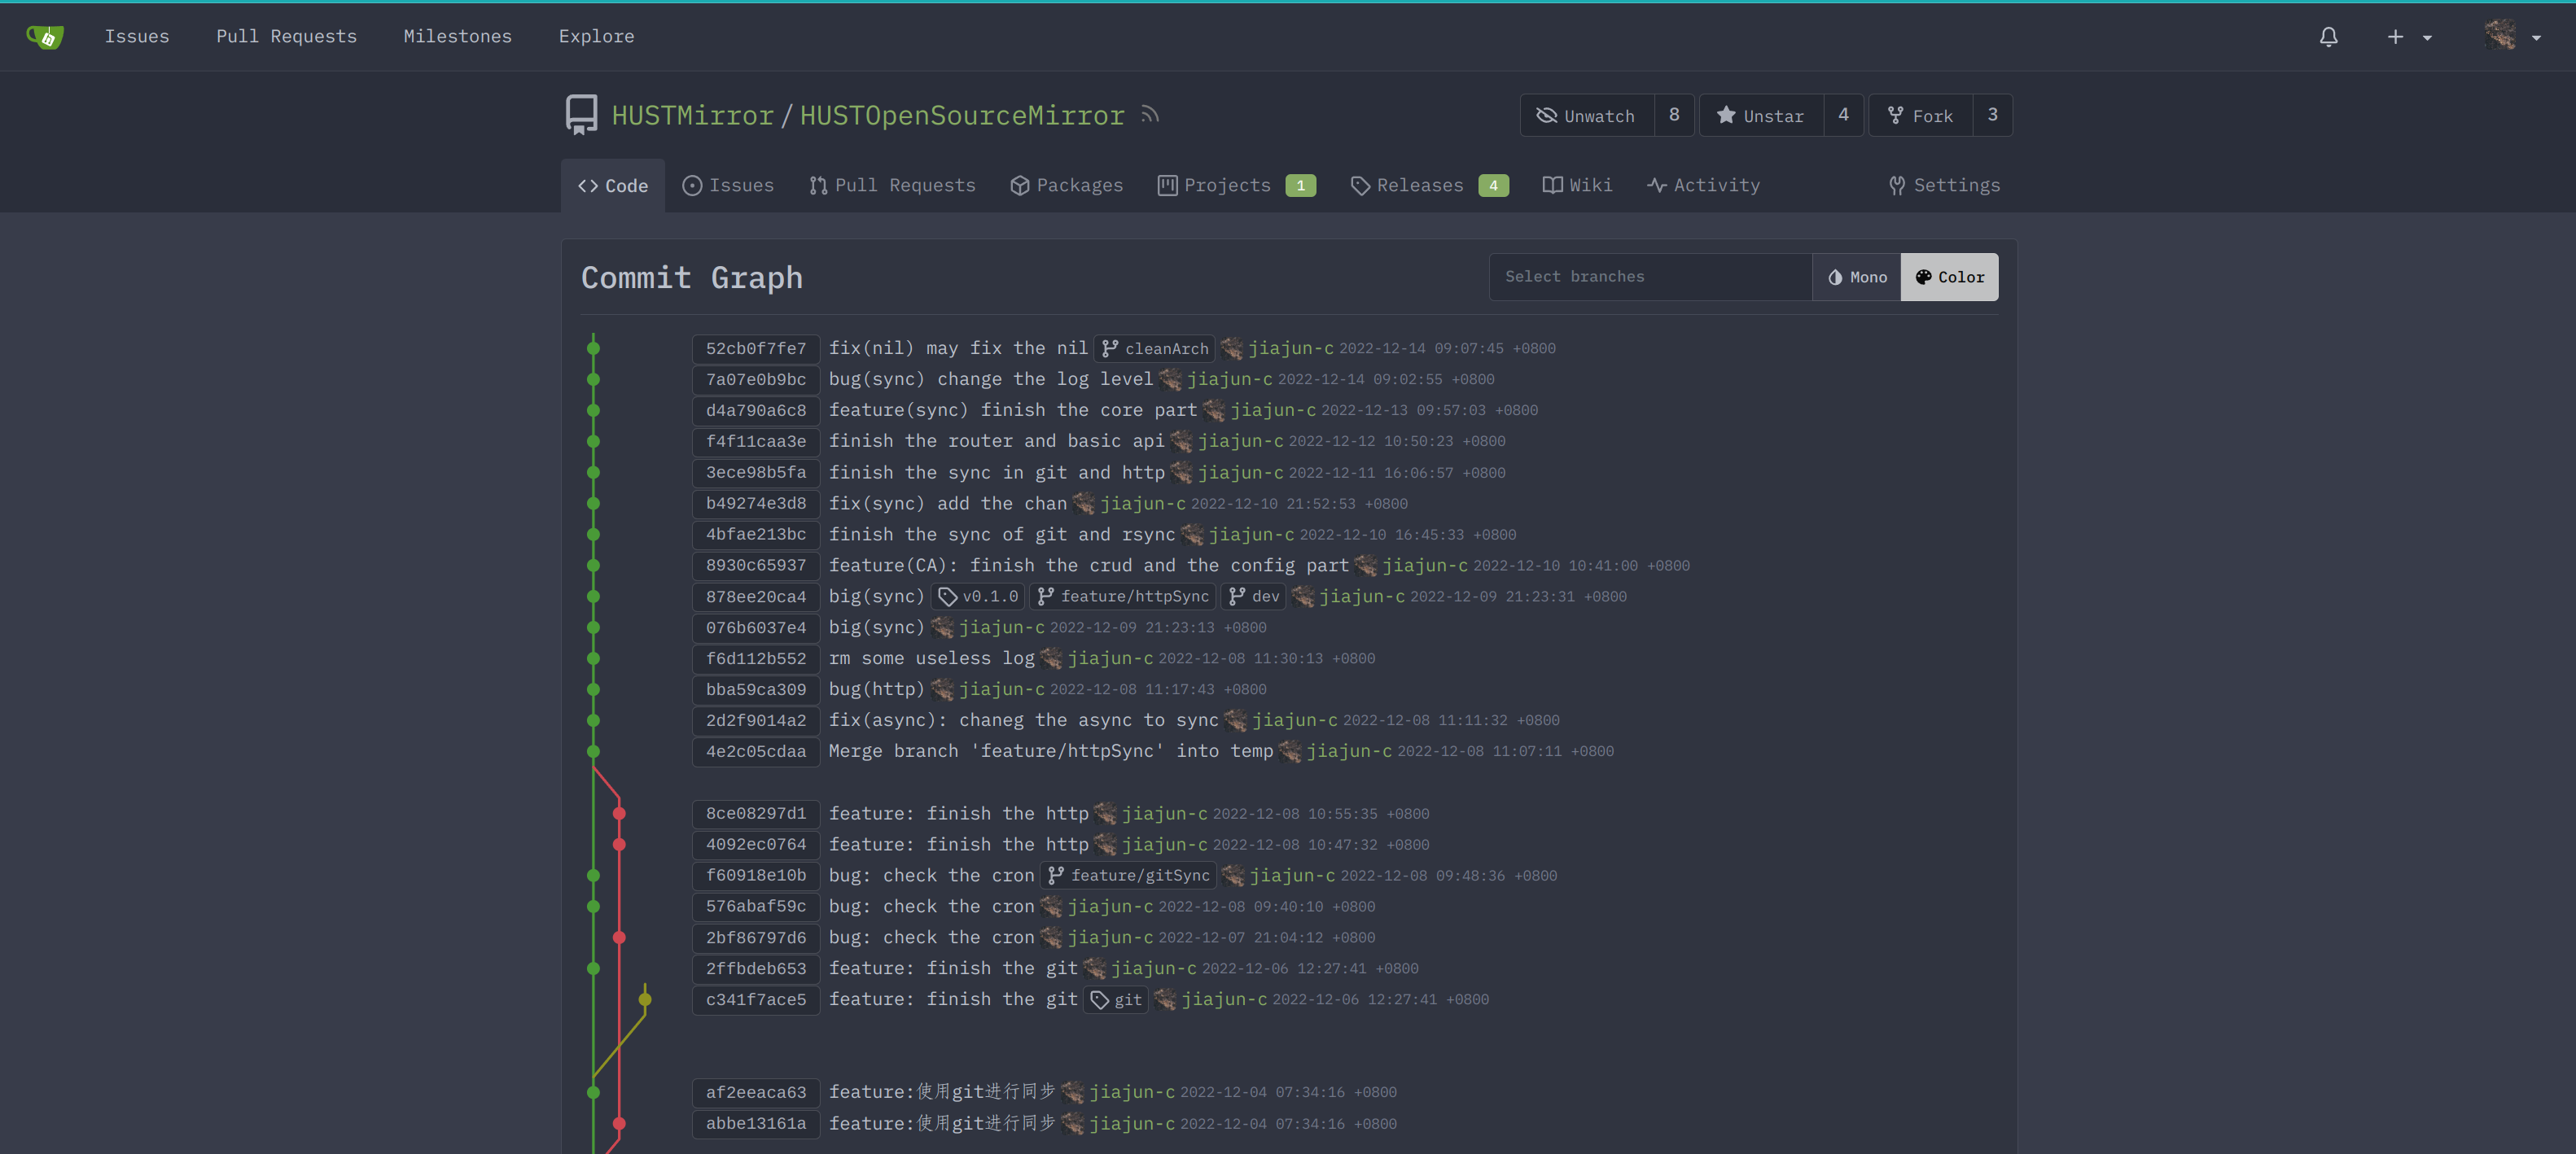
\includegraphics[width=1\textwidth]{./images/gitea.png}
    \caption{代码管理}
    \label{code}
\end{figure}

对于后端仓库commit情况,我一共提交了51次commit,发布了一个release
前端仓库仓库提交了51次commit, 目前正在用react重构中,该仓库不再更新,暂时未发布
release
\begin{figure}[!h]
    \centering
    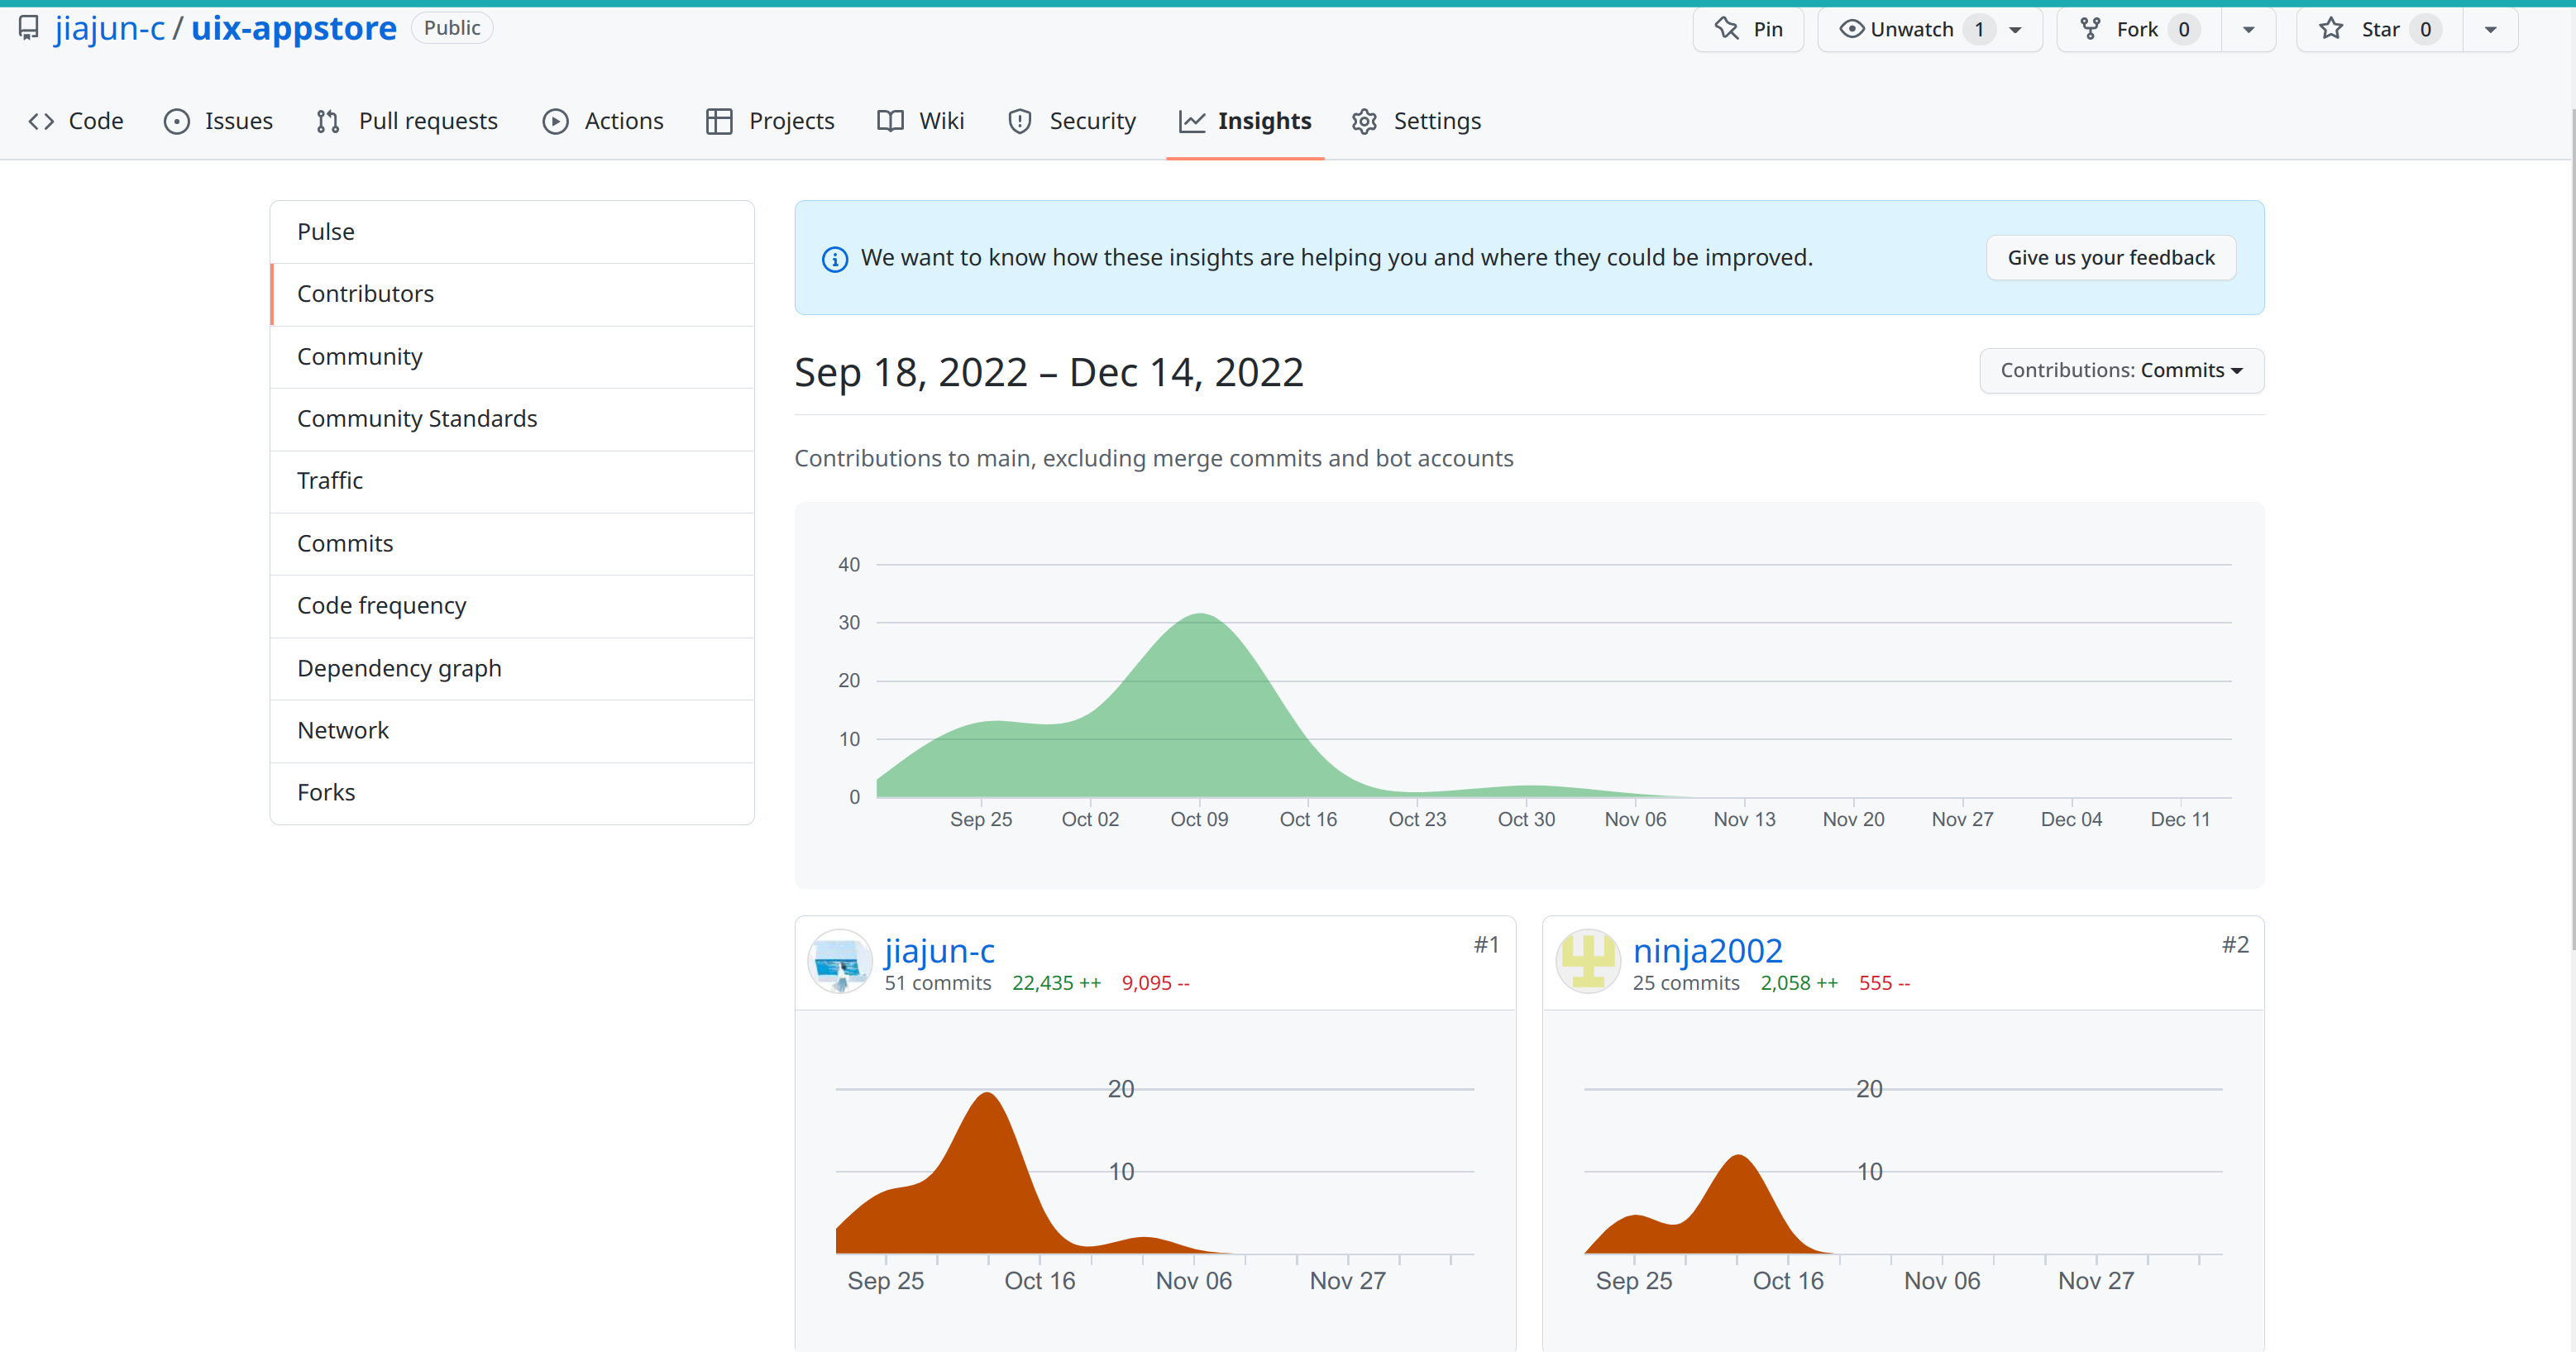
\includegraphics[width=0.8\textwidth]{./images/hust-front.png}
    \caption{前端仓库情况}
    \label{code}
\end{figure}
\newpage
\begin{figure}[!h]
    \centering
    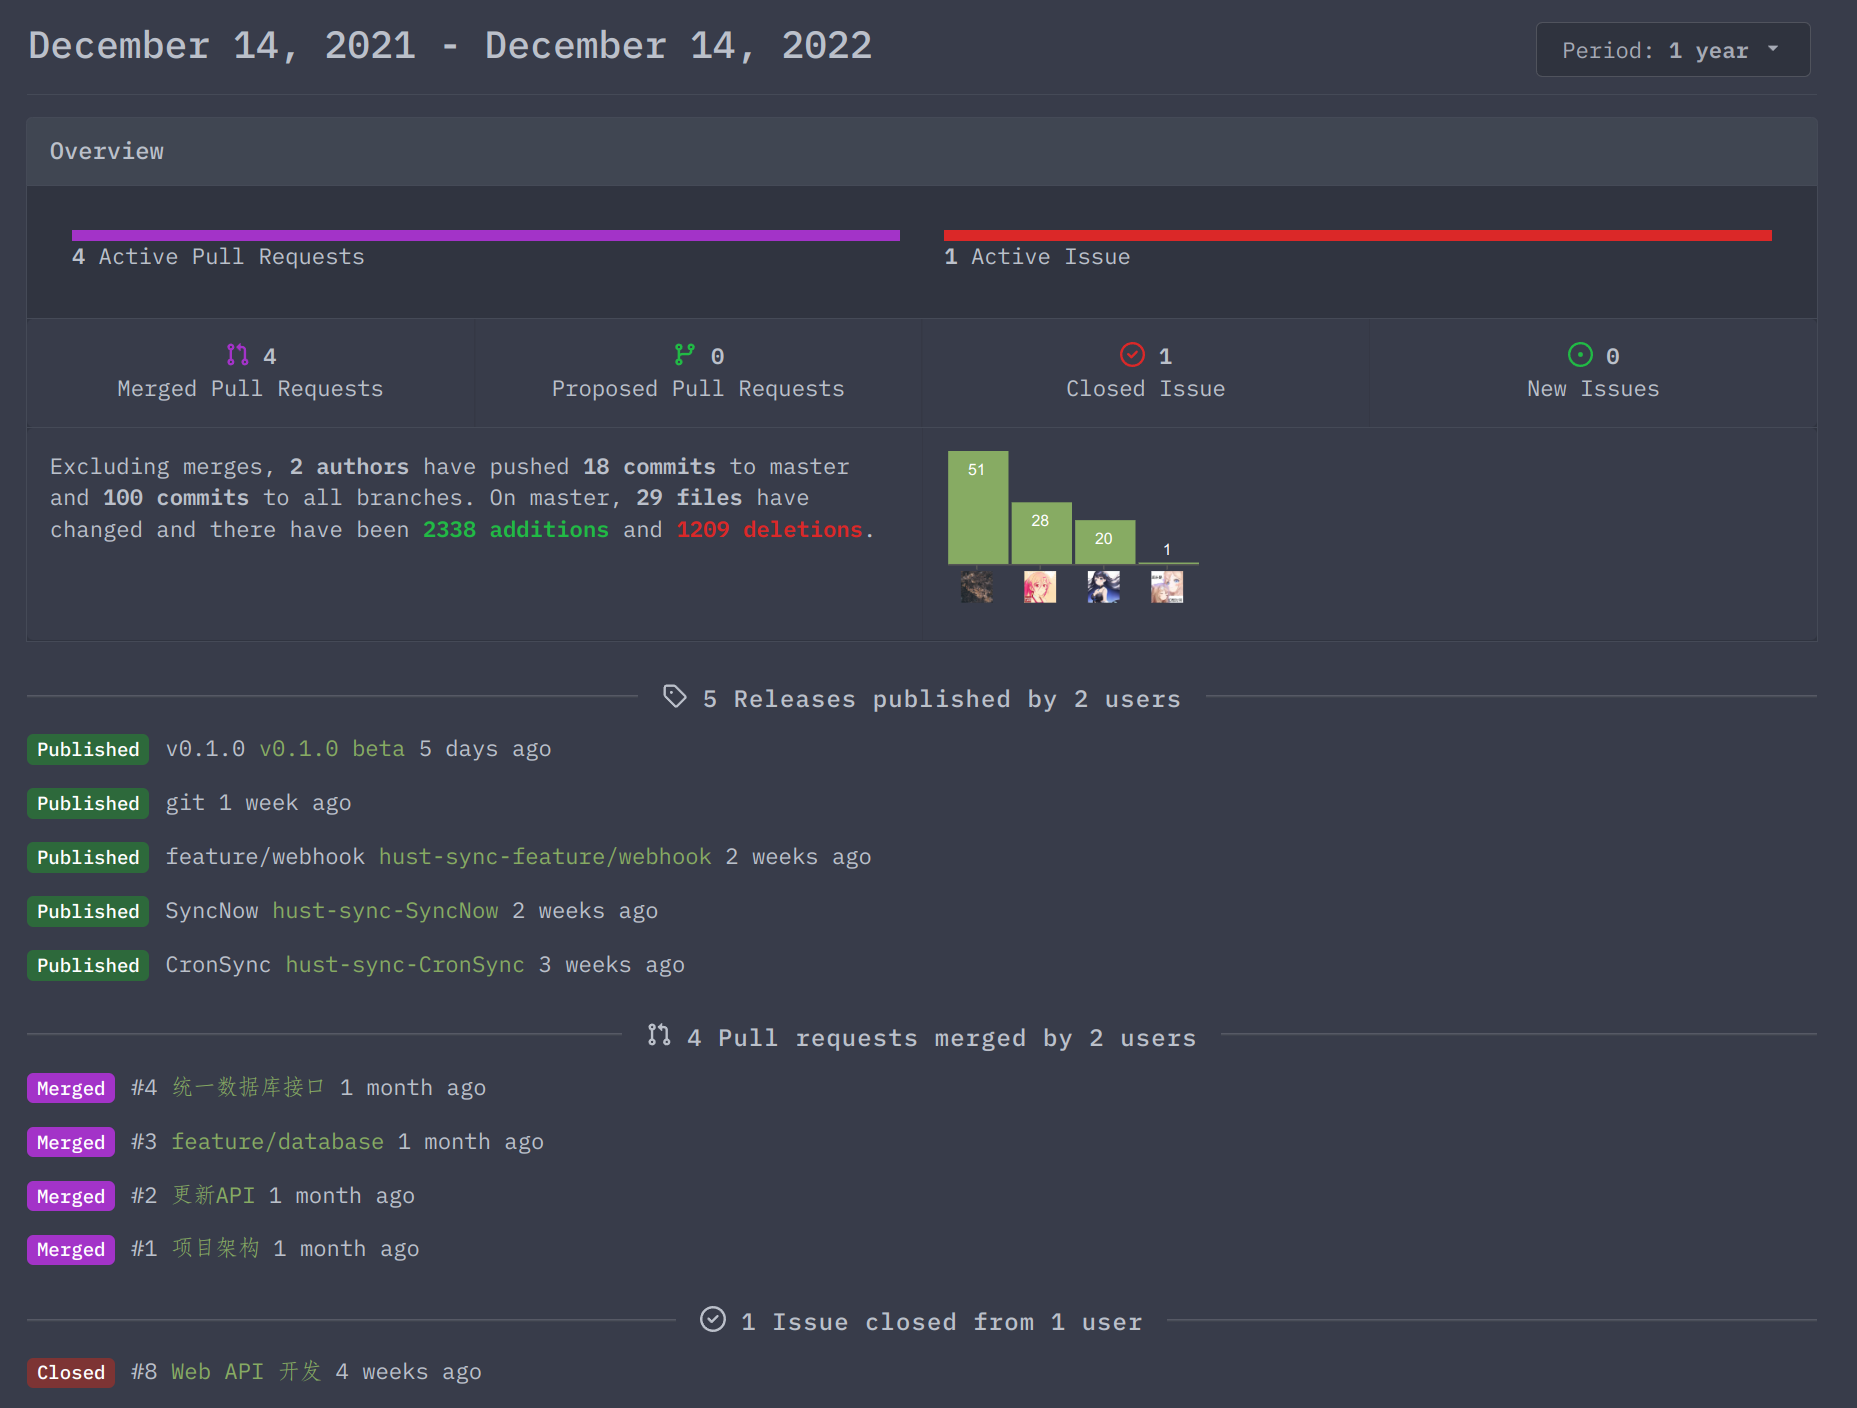
\includegraphics[width=1\textwidth]{./images/hust.png}
    \caption{后端仓库情况}
    \label{hust}
\end{figure}

\subsection{关键函数说明}

对于web api,通过Router函数进行设置,其又分为管理级别的API以及普通的API,

管理员级别的API后面应该进行鉴权防止意外错误,如图\ref{main} 所示。
\begin{figure}[!h]
    \centering
    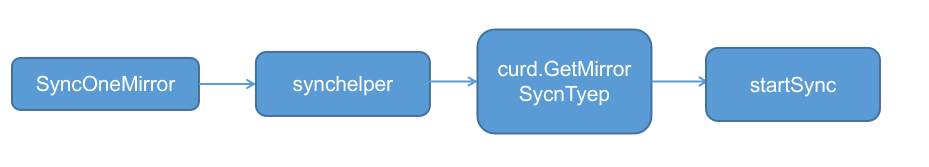
\includegraphics[width=1\textwidth]{./images/syncfunc.png}
    \caption{软件源同步}
    \label{syncm}
\end{figure}

对于软件源同步函数其调用逻辑如图\ref{syncm} 所示,SyncOneMirror将会开始
对一个软件源进行同步,该函数调用synchelper,随后再调用curd包中的GetMirrorSyncType获取
实现了同步接口的同步结构体,使用该同步函数进行同步。

\begin{figure}[!h]
    \centering
    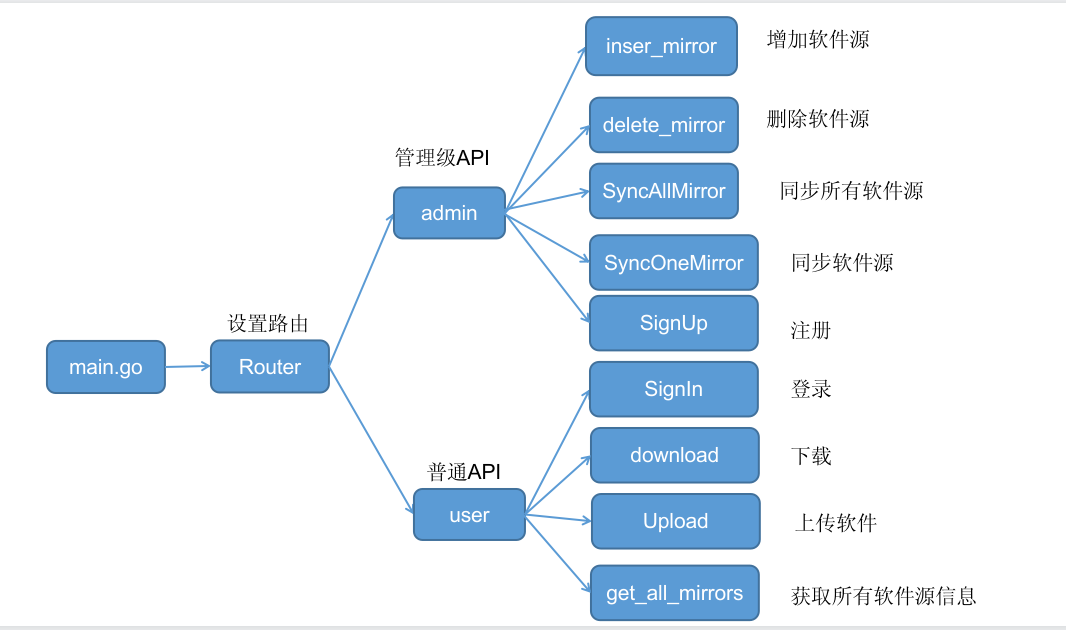
\includegraphics[width=1\textwidth]{./images/func.png}
    \caption{总体调用情况}
    \label{main}
\end{figure}
\newpage
日志部分的设置则如图\ref{log}所示,在log包下设置init函数,由于golang的语言特性,此时的init函数
将会被调用,在其中为不同LOG级别的日志设置输出文件。最终呈现的效果如图\ref{logrus} 所示。
\begin{figure}[!h]
    \centering
    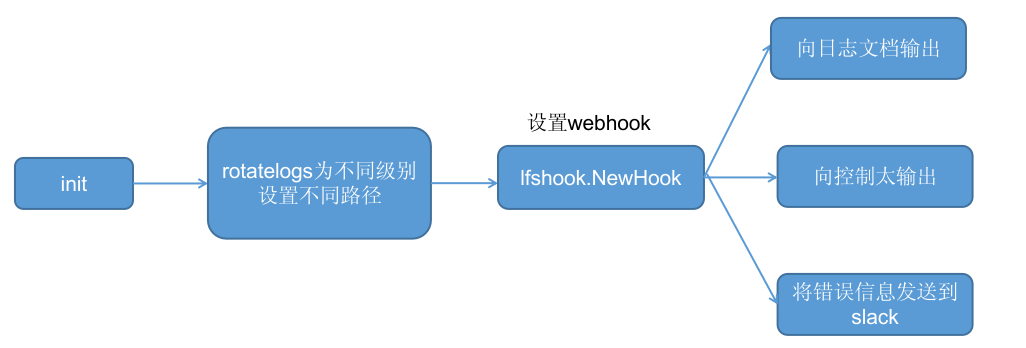
\includegraphics[width=1\textwidth]{./images/log.png}
    \caption{总体调用情况}
    \label{log}
\end{figure}

\begin{figure}[!h]
    \centering
    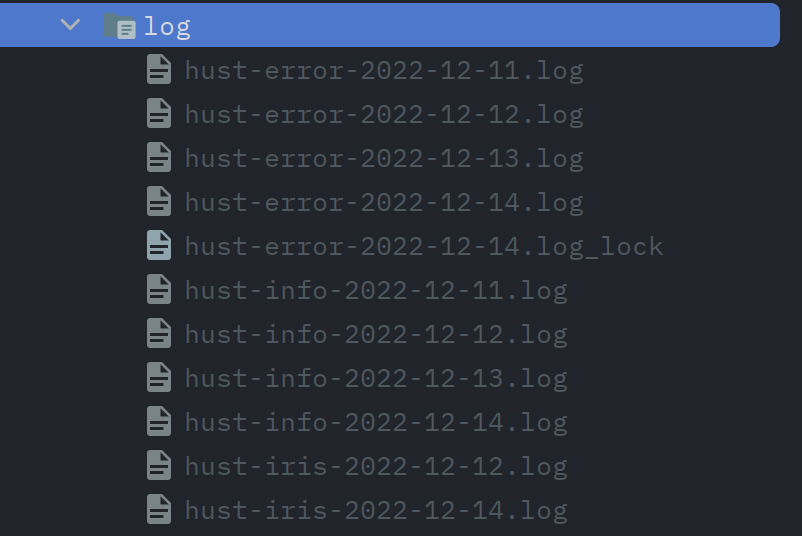
\includegraphics[width=0.5\textwidth]{./images/logrus.png}
    \caption{日志模块}
    \label{logrus}
\end{figure}

软件的上传下载调用逻辑如图\ref{updown} 所示,在下载的时候首先调用crud中的GetSoftwarePath获取在本地的逻辑,
随后使用iris中的sendFile方法发送软件到客户端。

在上传的时候,首先会检查是否在远端存在,如果存在的时候进行更新,如果不存在那么将会进行创建。在数据库中进行记录。


\begin{figure}[!h]
    \centering
    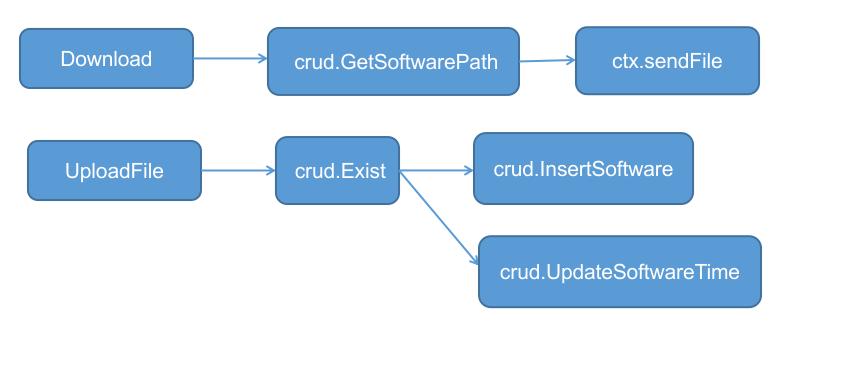
\includegraphics[width=1\textwidth]{./images/down.png}
    \caption{软件上传下载}
    \label{updown}
\end{figure}

\subsection{测试计划和测试用例}
\subsubsection{测试方法}
在测试的过程中分为单元测试和自动化测试,自动化测试使用drone进行操作,drone如图\ref{drone}所示。
\begin{figure}[!h]
    \centering
    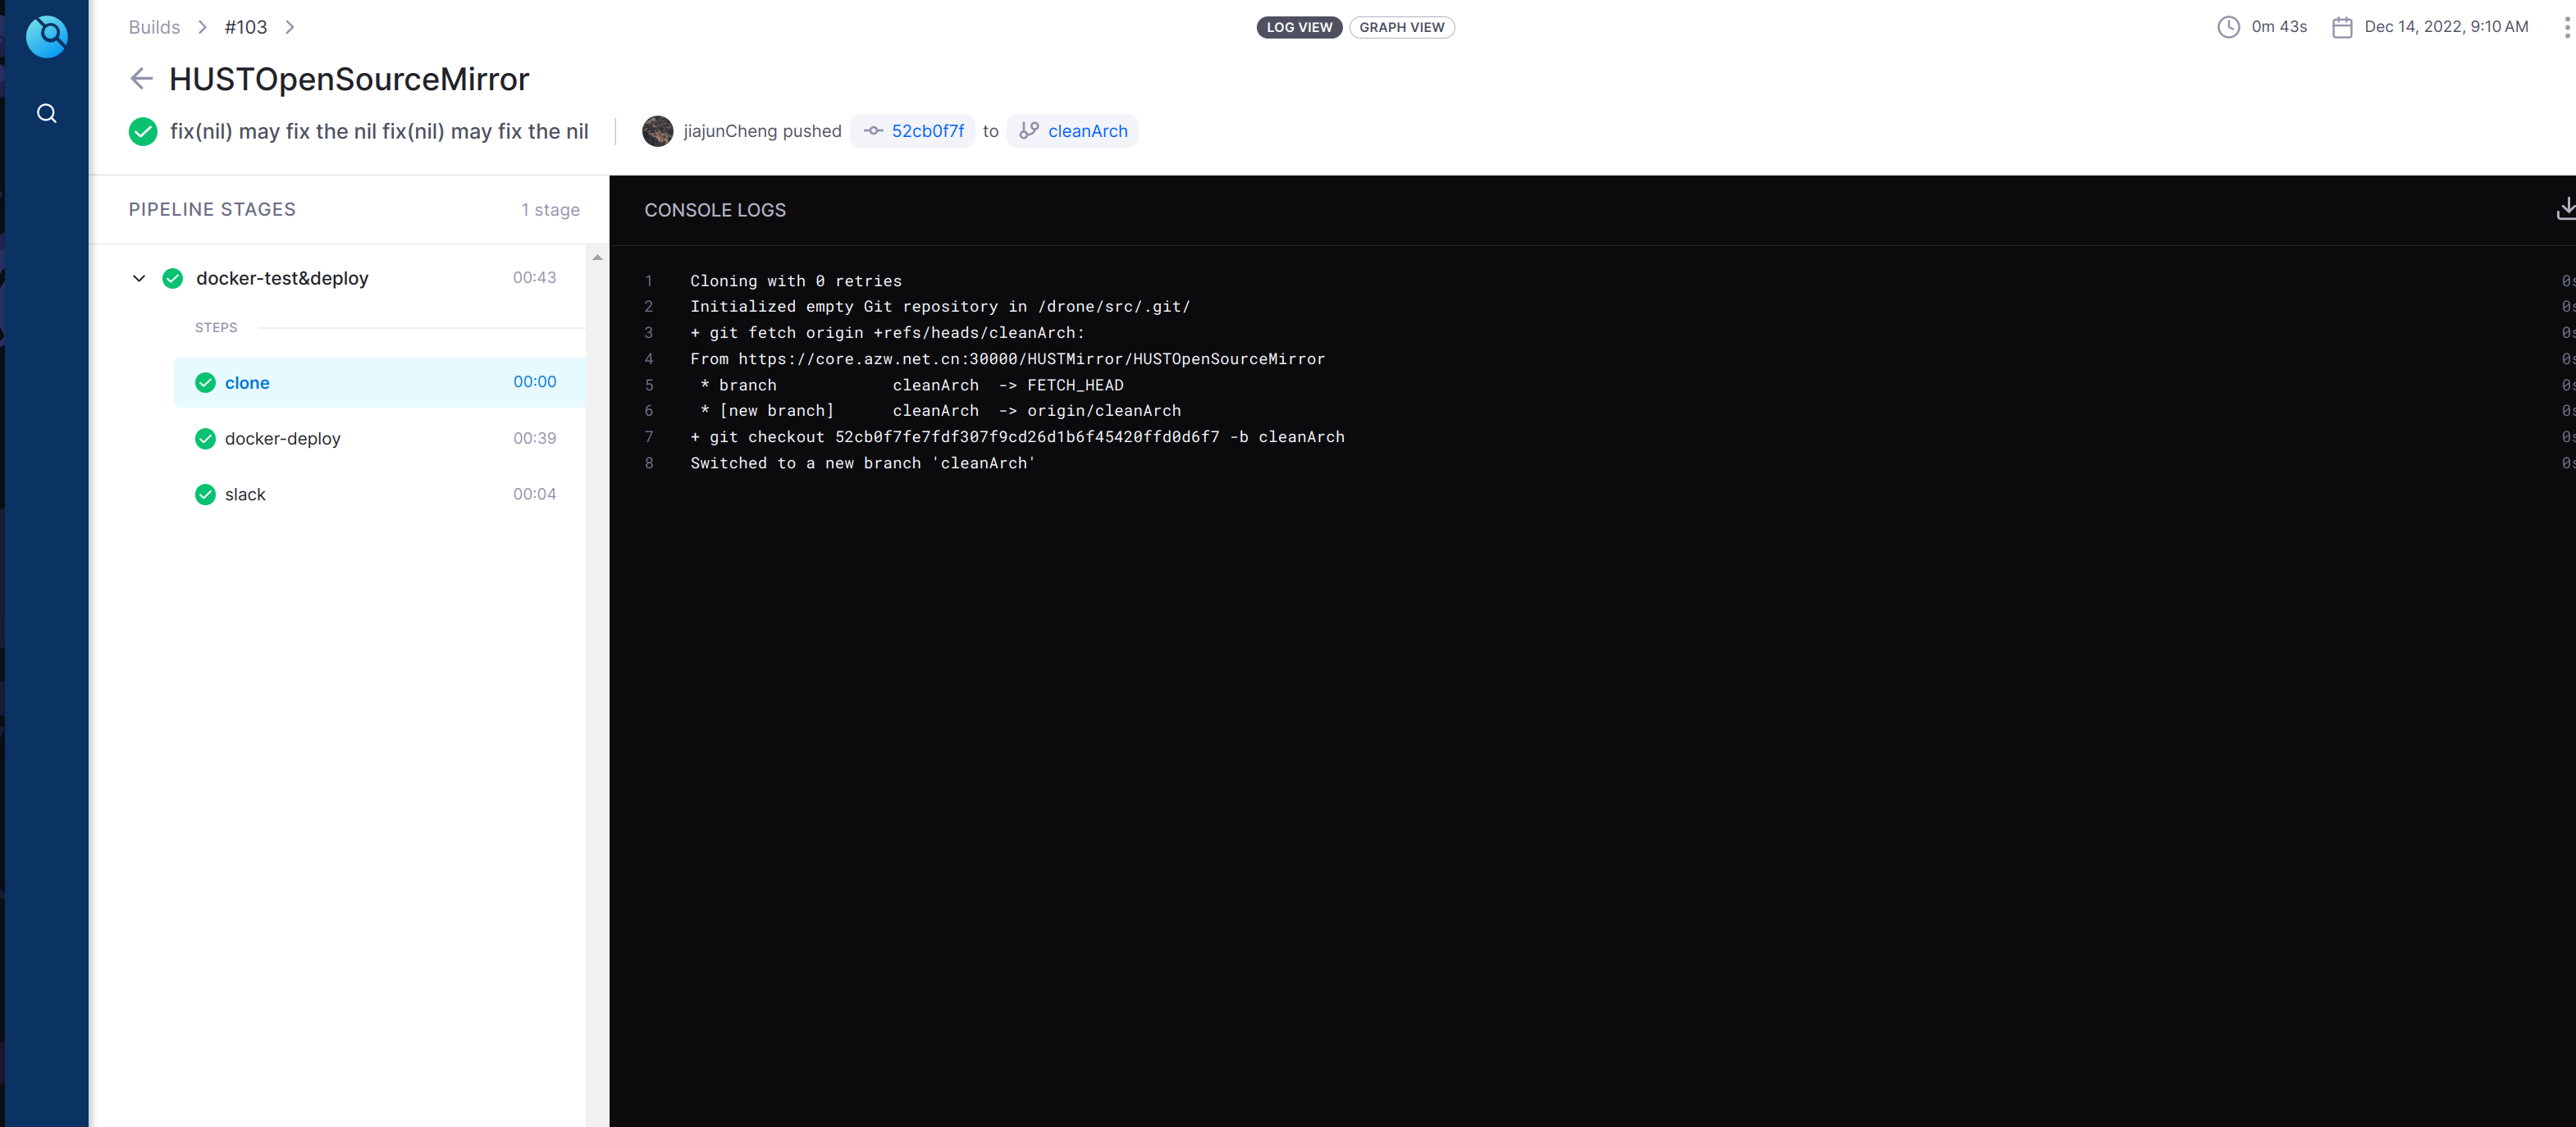
\includegraphics[width=1\textwidth]{./images/drone.png}
    \caption{drone}
    \label{drone}
\end{figure}
\newpage

当自动编译部署通过后将会发送信息到slack中
\begin{figure}[!h]
    \centering
    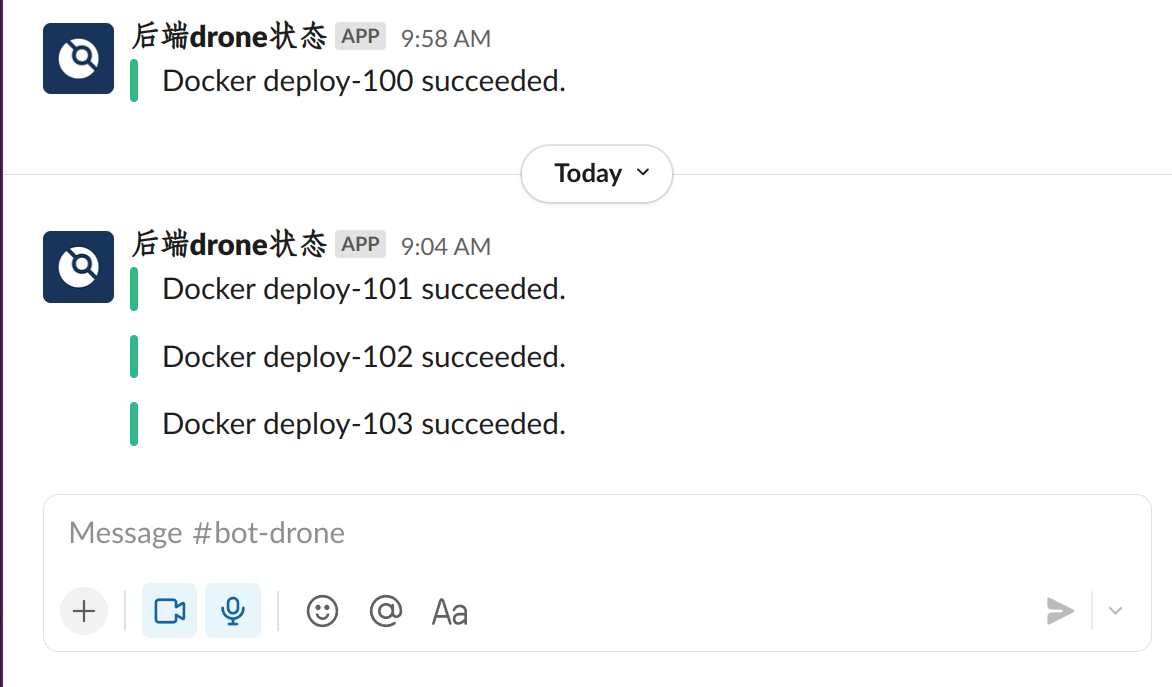
\includegraphics[width=1\textwidth]{./images/drone-bot.png}
    \caption{drone slack通知}
    \label{slack}
\end{figure}

对于普通函数的测试,使用go自带的test包进行测试,如图\ref{go-test} 所示。
\begin{figure}[!h]
    \centering
    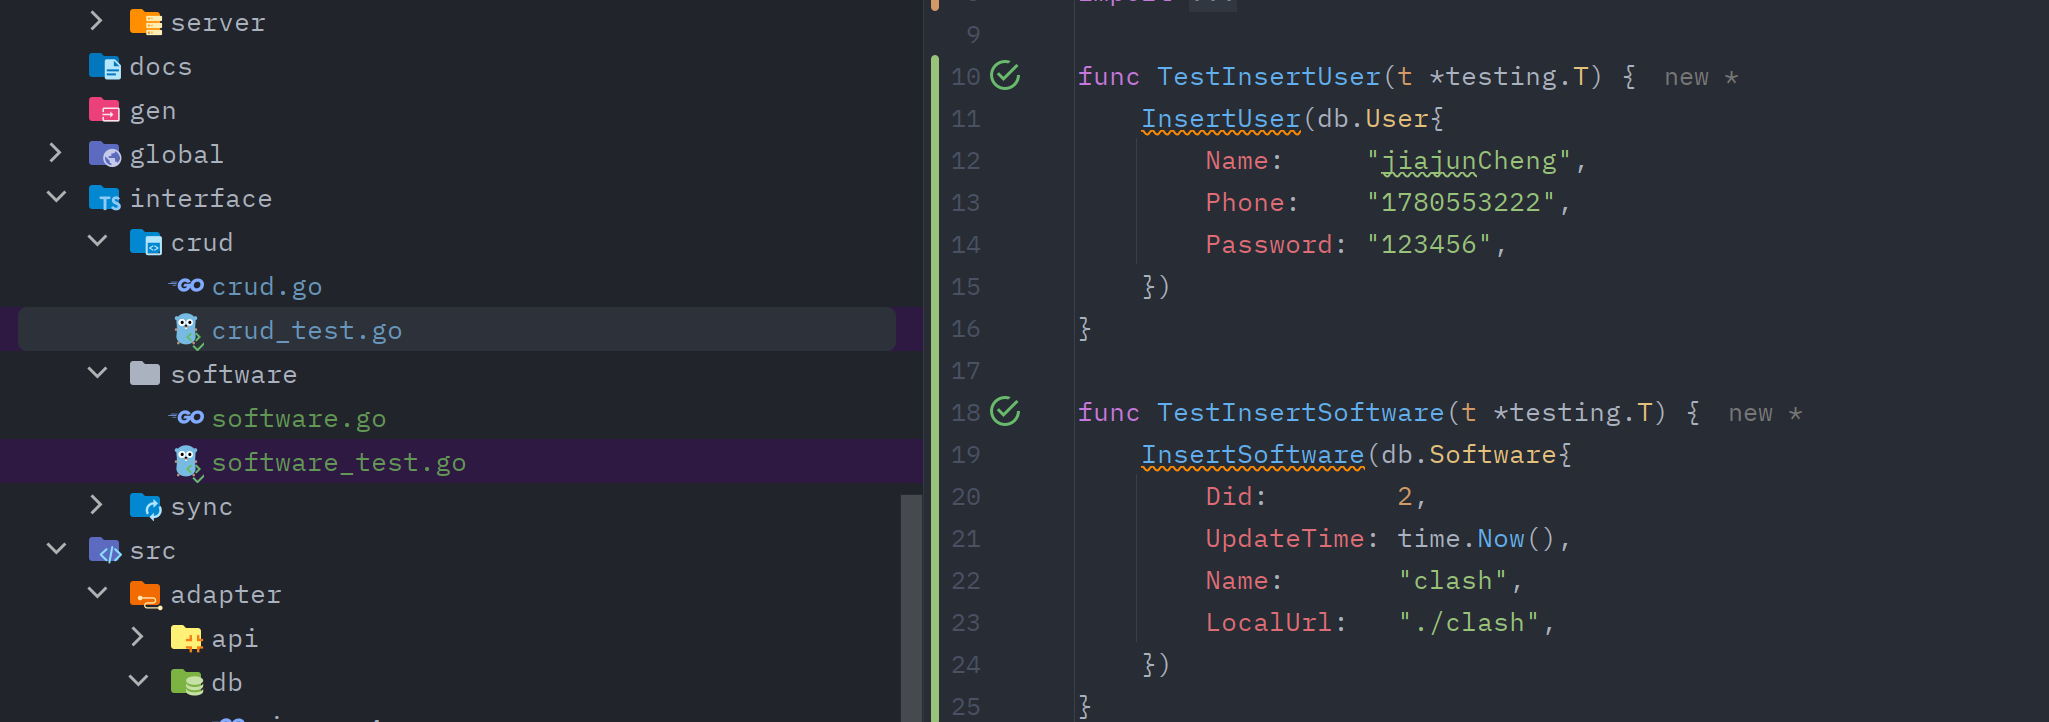
\includegraphics[width=1\textwidth]{./images/test.png}
    \caption{go单元测试}
    \label{go-test}
\end{figure}

对于api的测试,使用Postman进行测试,根据测试的返回结果判断测试结果。
\newpage
\begin{figure}[!h]
    \centering
    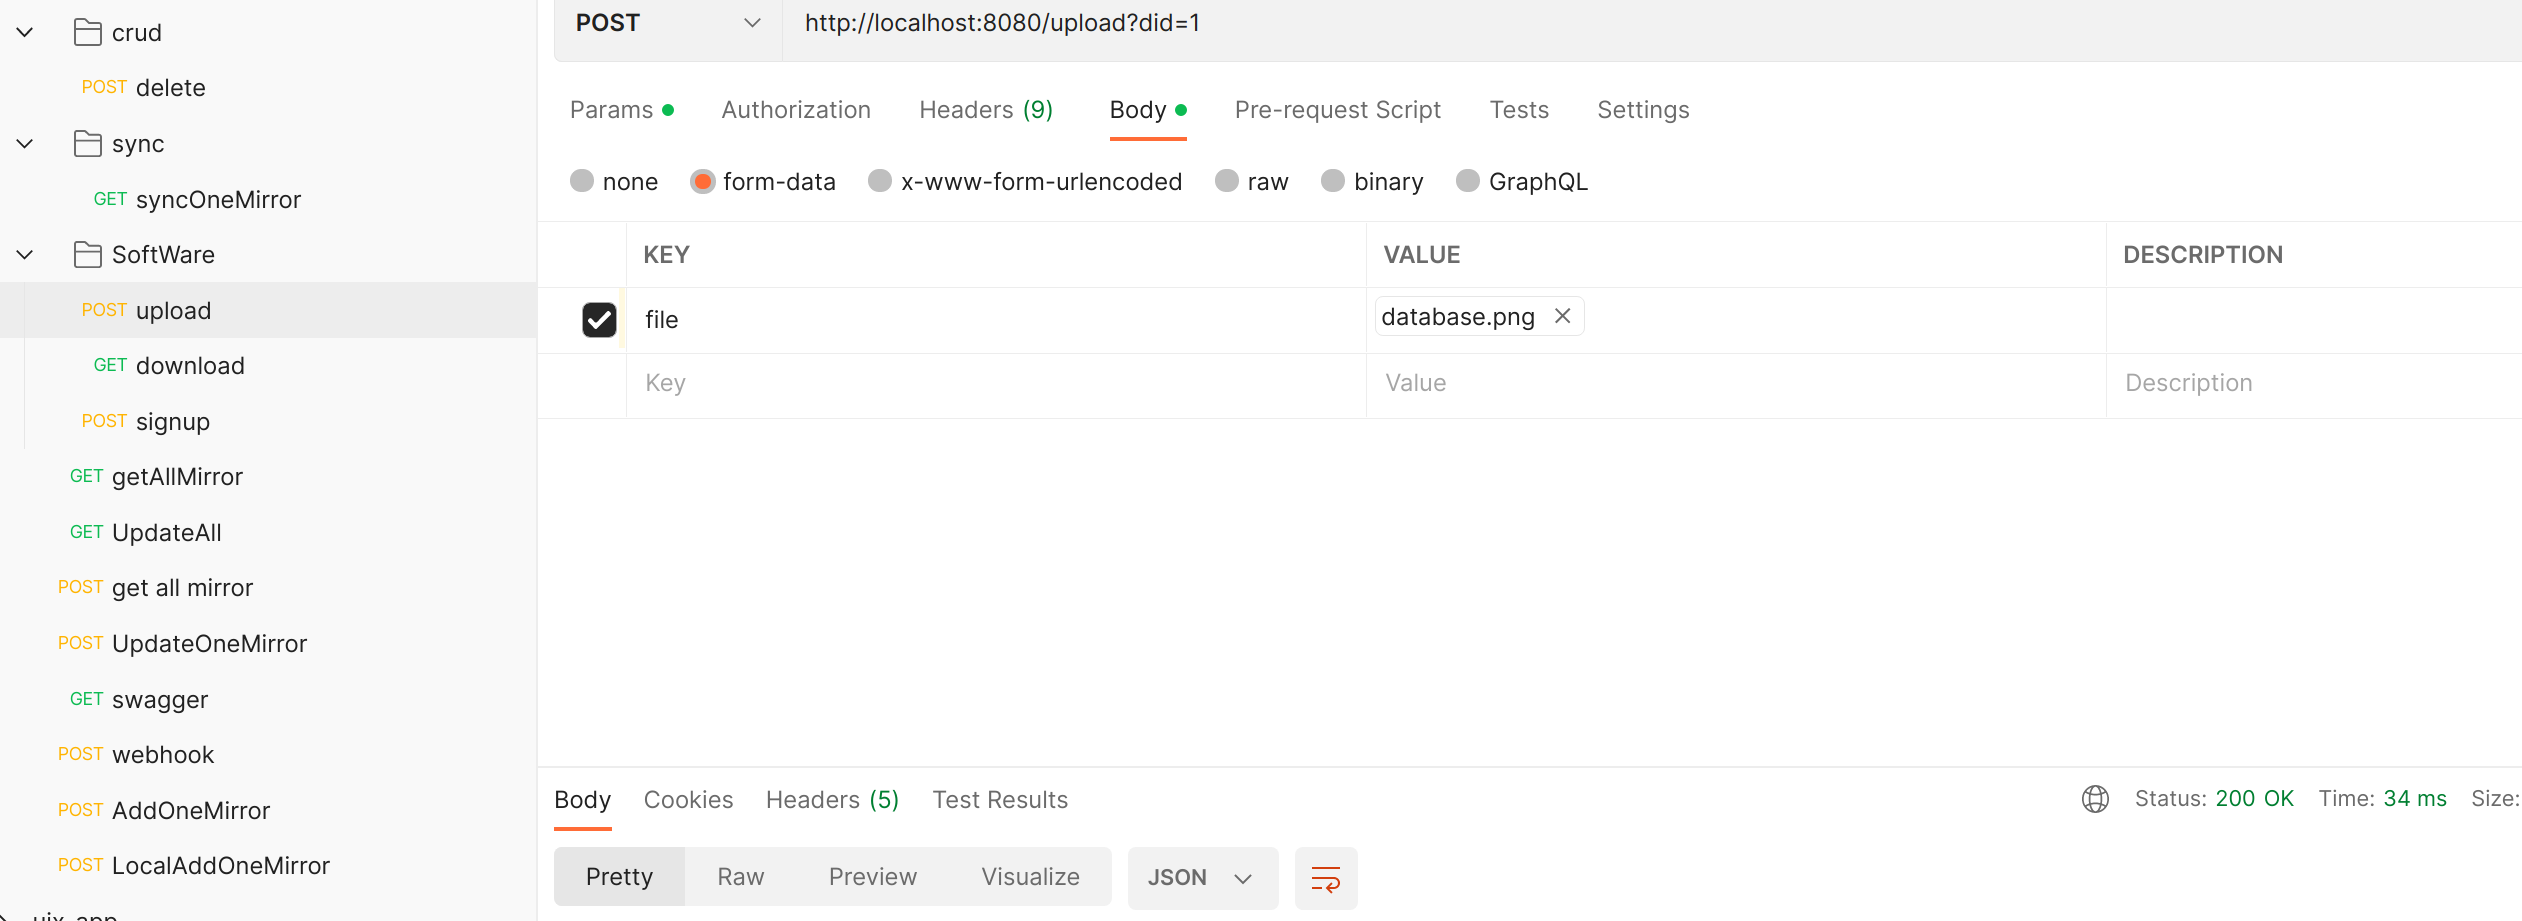
\includegraphics[width=1\textwidth]{./images/api_test.png}
    \caption{api单元测试}
    \label{api-test}
\end{figure}

\subsubsection{测试用例}
软件源同步功能测试,在这里我们选择git方式进行同步,在这里我们选取一个gitee上的项目进行同步,发现
此时目录下面已经存在该repo,如图\ref{sync-git} 所示。
\begin{figure}[!h]
    \centering
    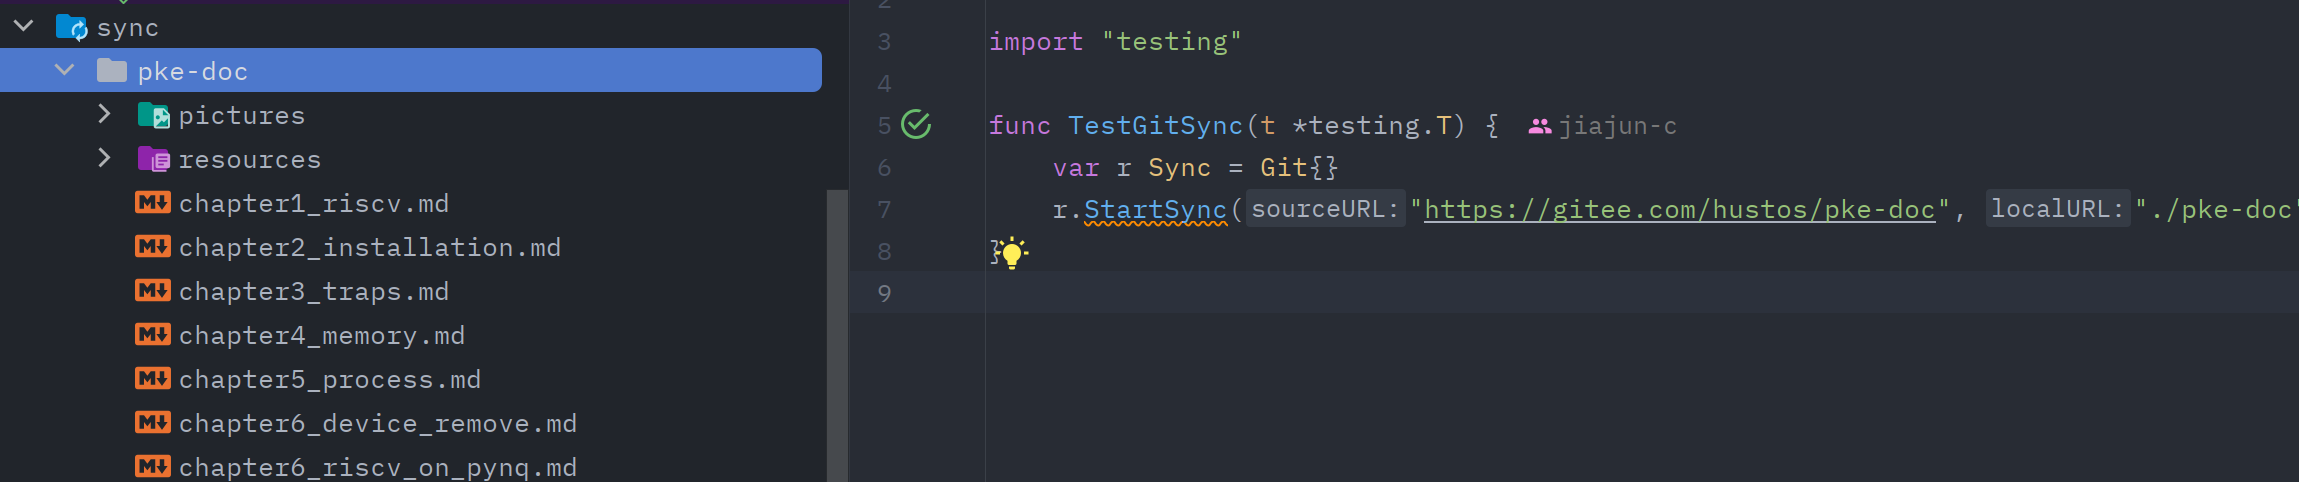
\includegraphics[width=1\textwidth]{./images/git.png}
    \caption{同步功能测试}
    \label{sync-git}
\end{figure}

软件上传功能测试,如图\ref{upload}所示,将本地的一个图片上传到远端,发现此时uploads文件下面已经存在了该文件,
如图\ref{upload-res} 所示。
\begin{figure}[!h]
    \centering
    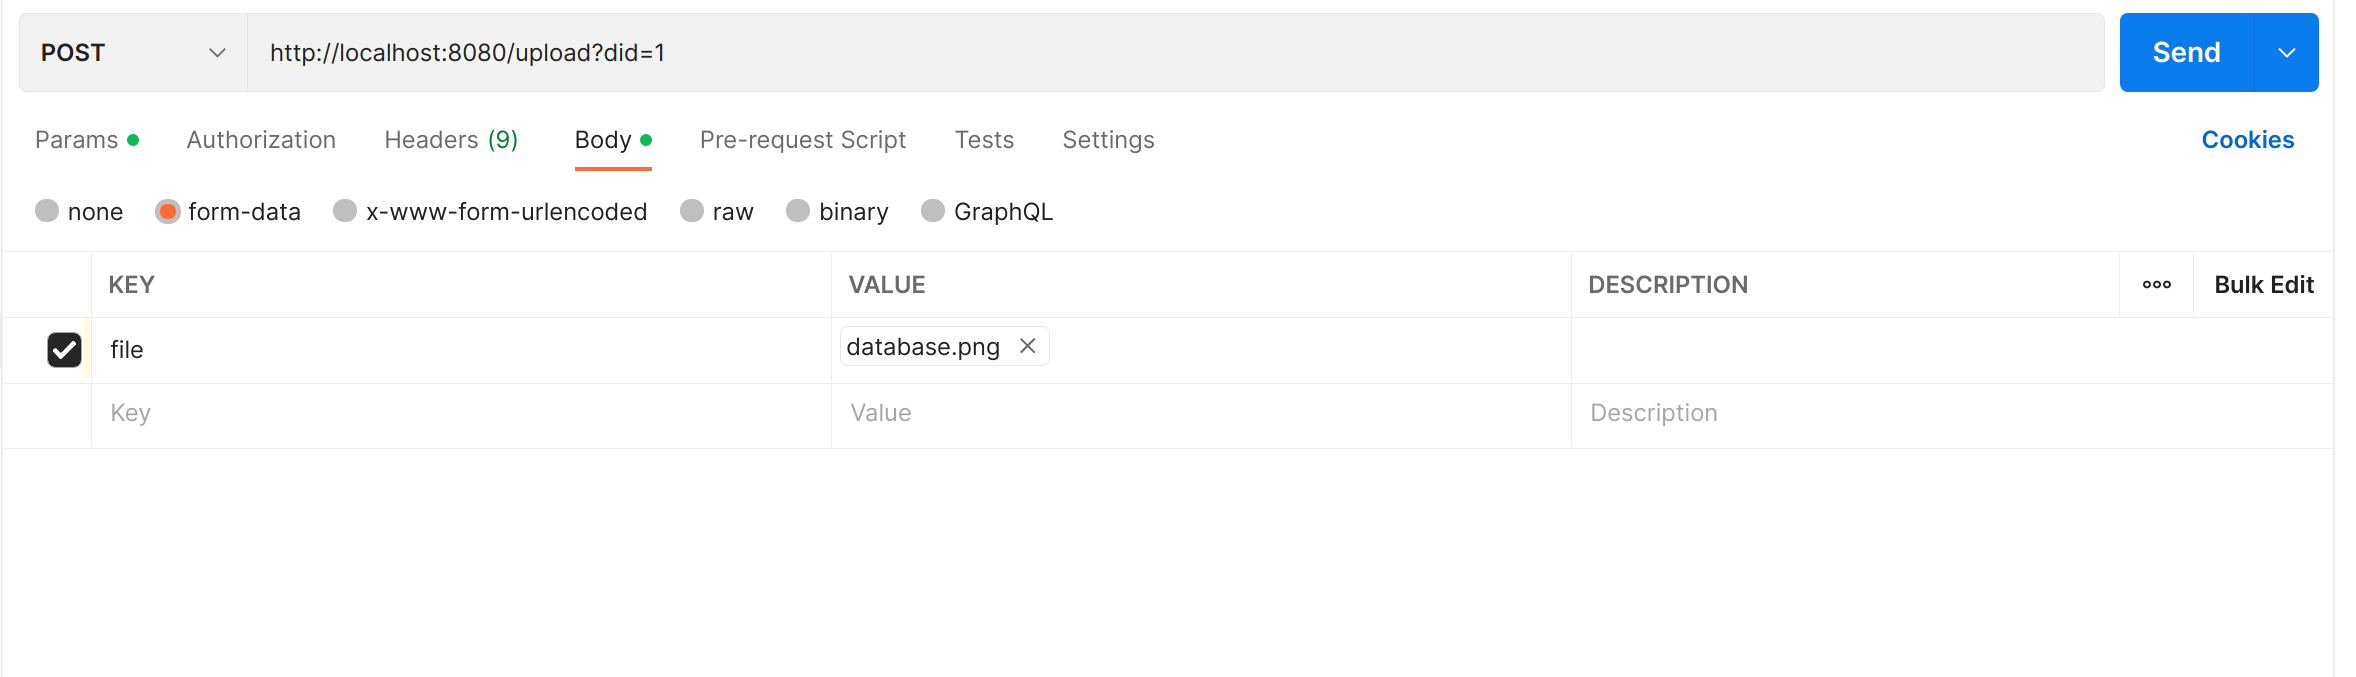
\includegraphics[width=1\textwidth]{./images/upload.png}
    \caption{上传功能测试}
    \label{upload}
\end{figure}
\newpage
\begin{figure}[!h]
    \centering
    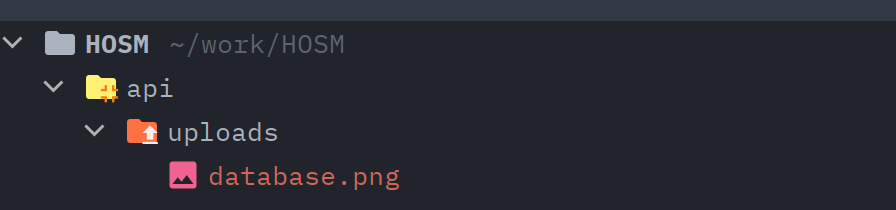
\includegraphics[width=0.7\textwidth]{./images/upload-res.png}
    \caption{上传功能测试结果}
    \label{upload-res}
\end{figure}

用户注册功能测试,如图\ref{signup}所示
\begin{figure}[!h]
    \centering
    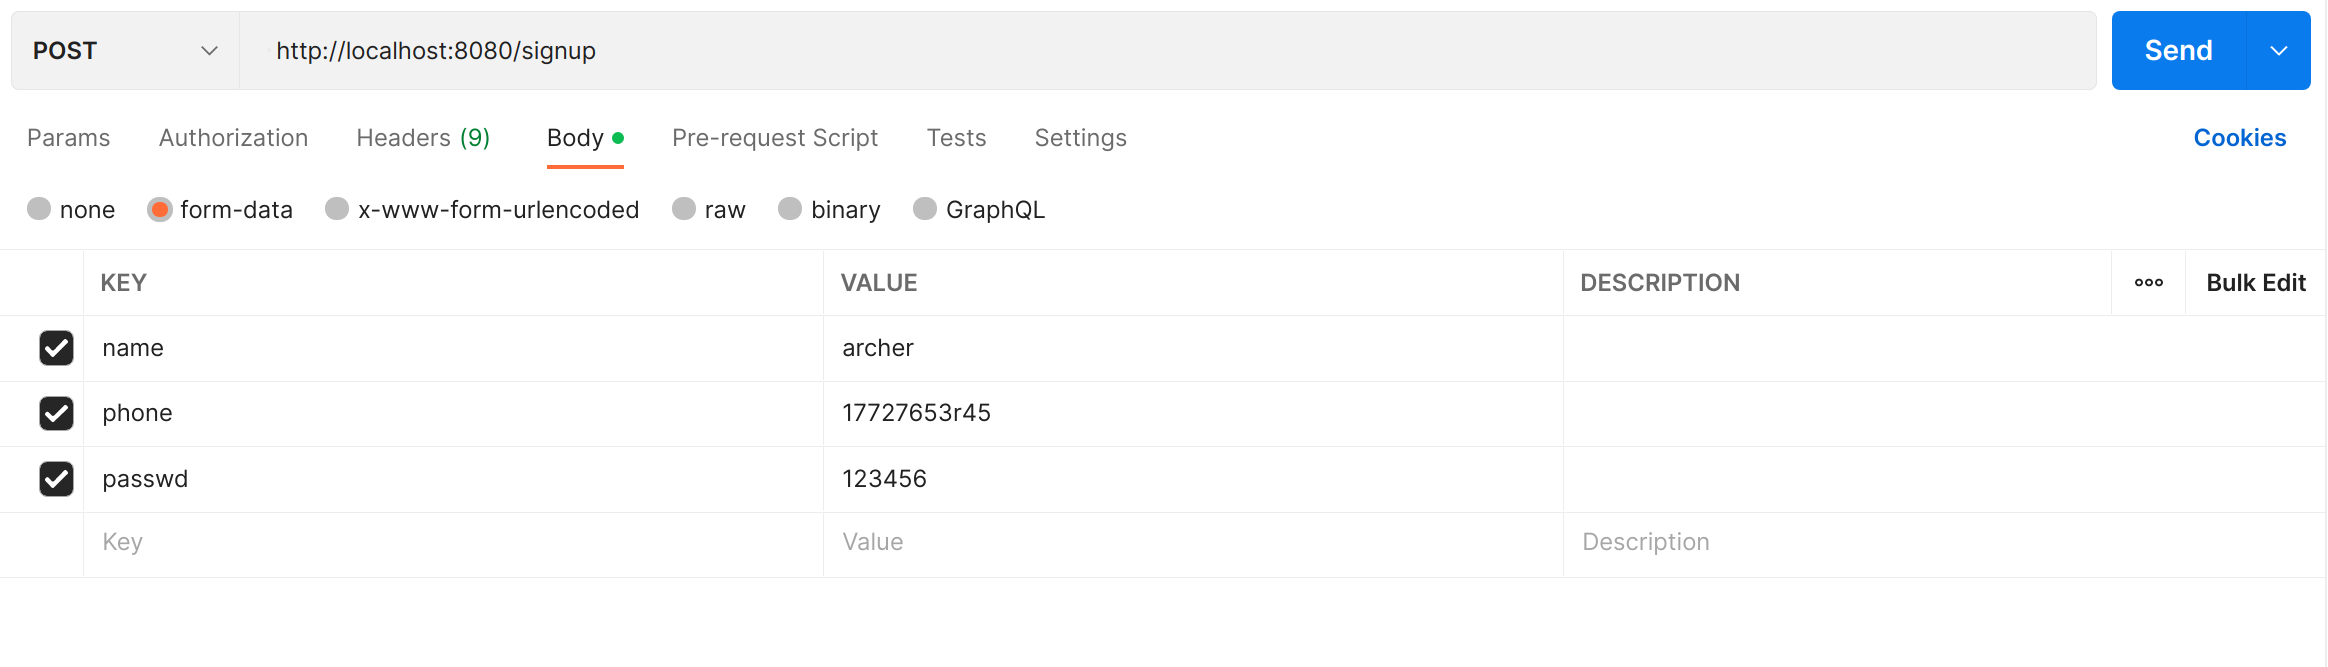
\includegraphics[width=1\textwidth]{./images/signup.png}
    \caption{注册功能}
    \label{signup}
\end{figure}

用户注册功能,测试结果如图\ref{signup-res} 所示,用户数据正常插入,数据库中存在该记录。
\begin{figure}[!h]
    \centering
    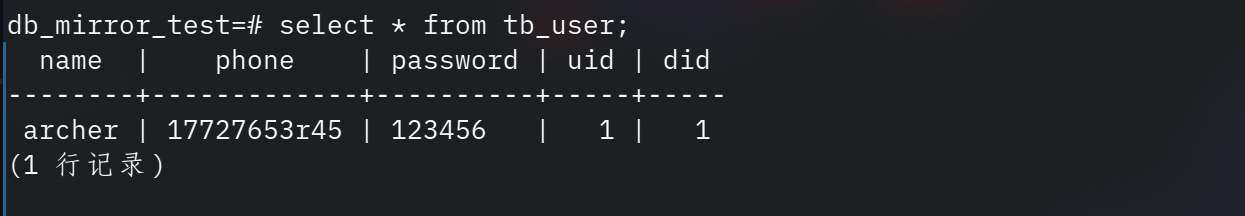
\includegraphics[width=1\textwidth]{./images/signup_res.png}
    \caption{注册功能测试结果}
    \label{signup-res}
\end{figure}
\nocite{*} %% 作用是不对文献进行引用,但可以生成文献列表

%\bibliographystyle{HustGraduPaper}
%\bibliography{HustGraduPaper}

软件下载测试,使用clash软件进行测试(测试平台需要为archlinux),测试结果如图\ref{down-res}所示,点击下载后本地会有该软件存在。
\begin{figure}[!h]
    \centering
    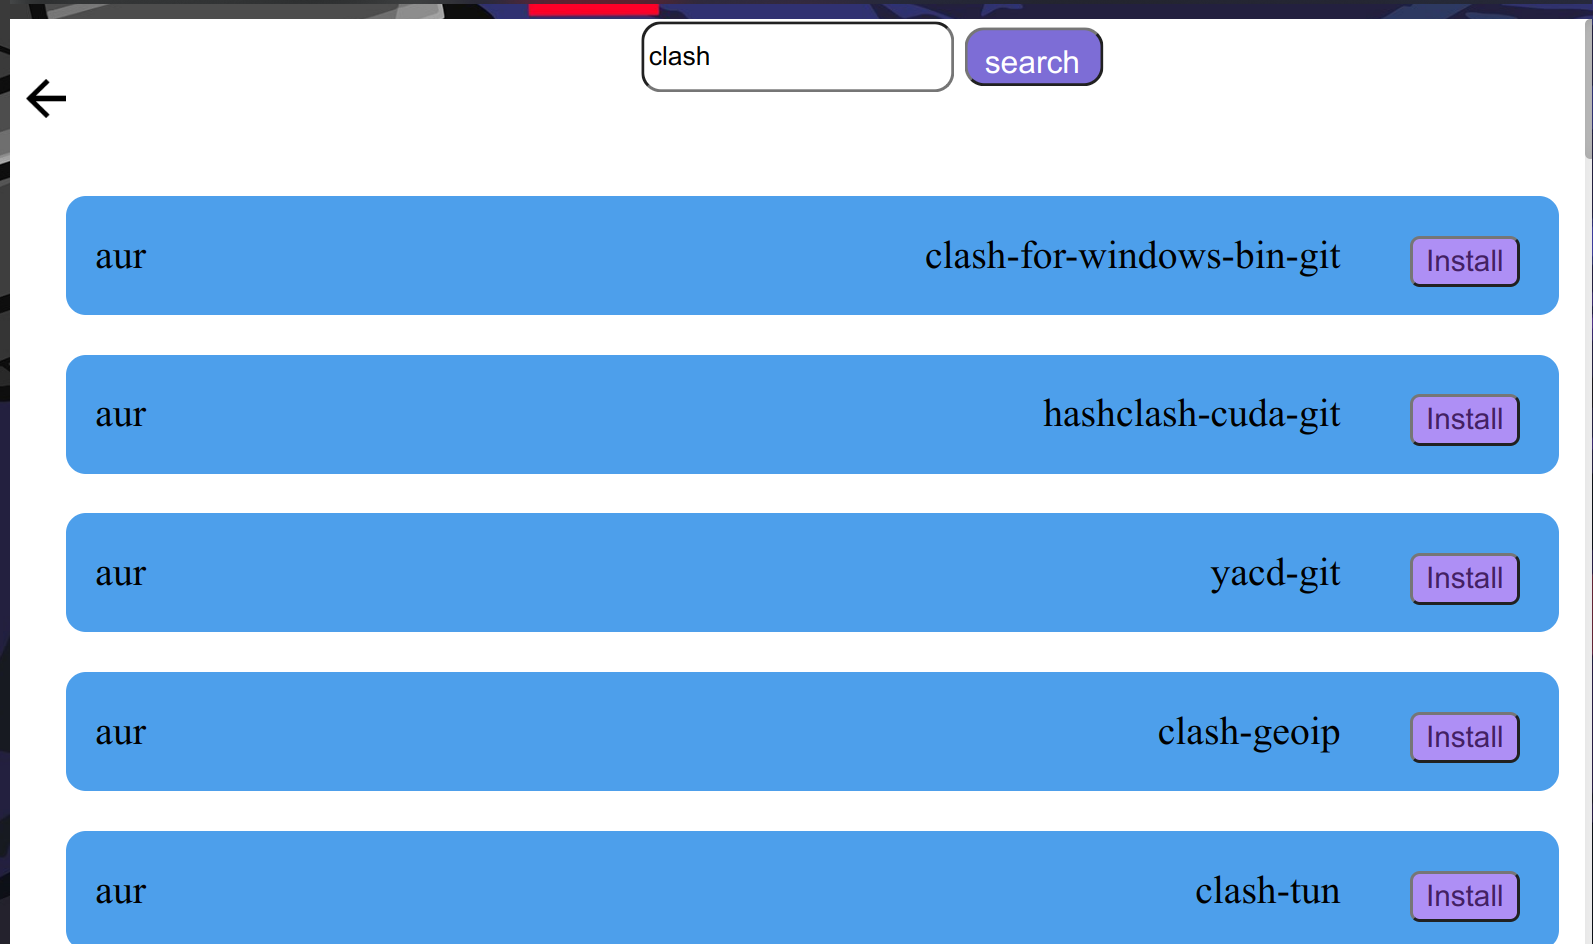
\includegraphics[width=0.7\textwidth]{./images/clash.png}
    \caption{软件下载功能测试结果}
    \label{down-res}
\end{figure}

\subsection{结果分析}
运行的结果满足我们的需求,和测试预期符合

\section{总结}
\subsection{用户反馈}
本次的后端已经复用于HLUG开源镜像站测试中,如图\ref{front}所示

\begin{figure}[!h]
    \centering
    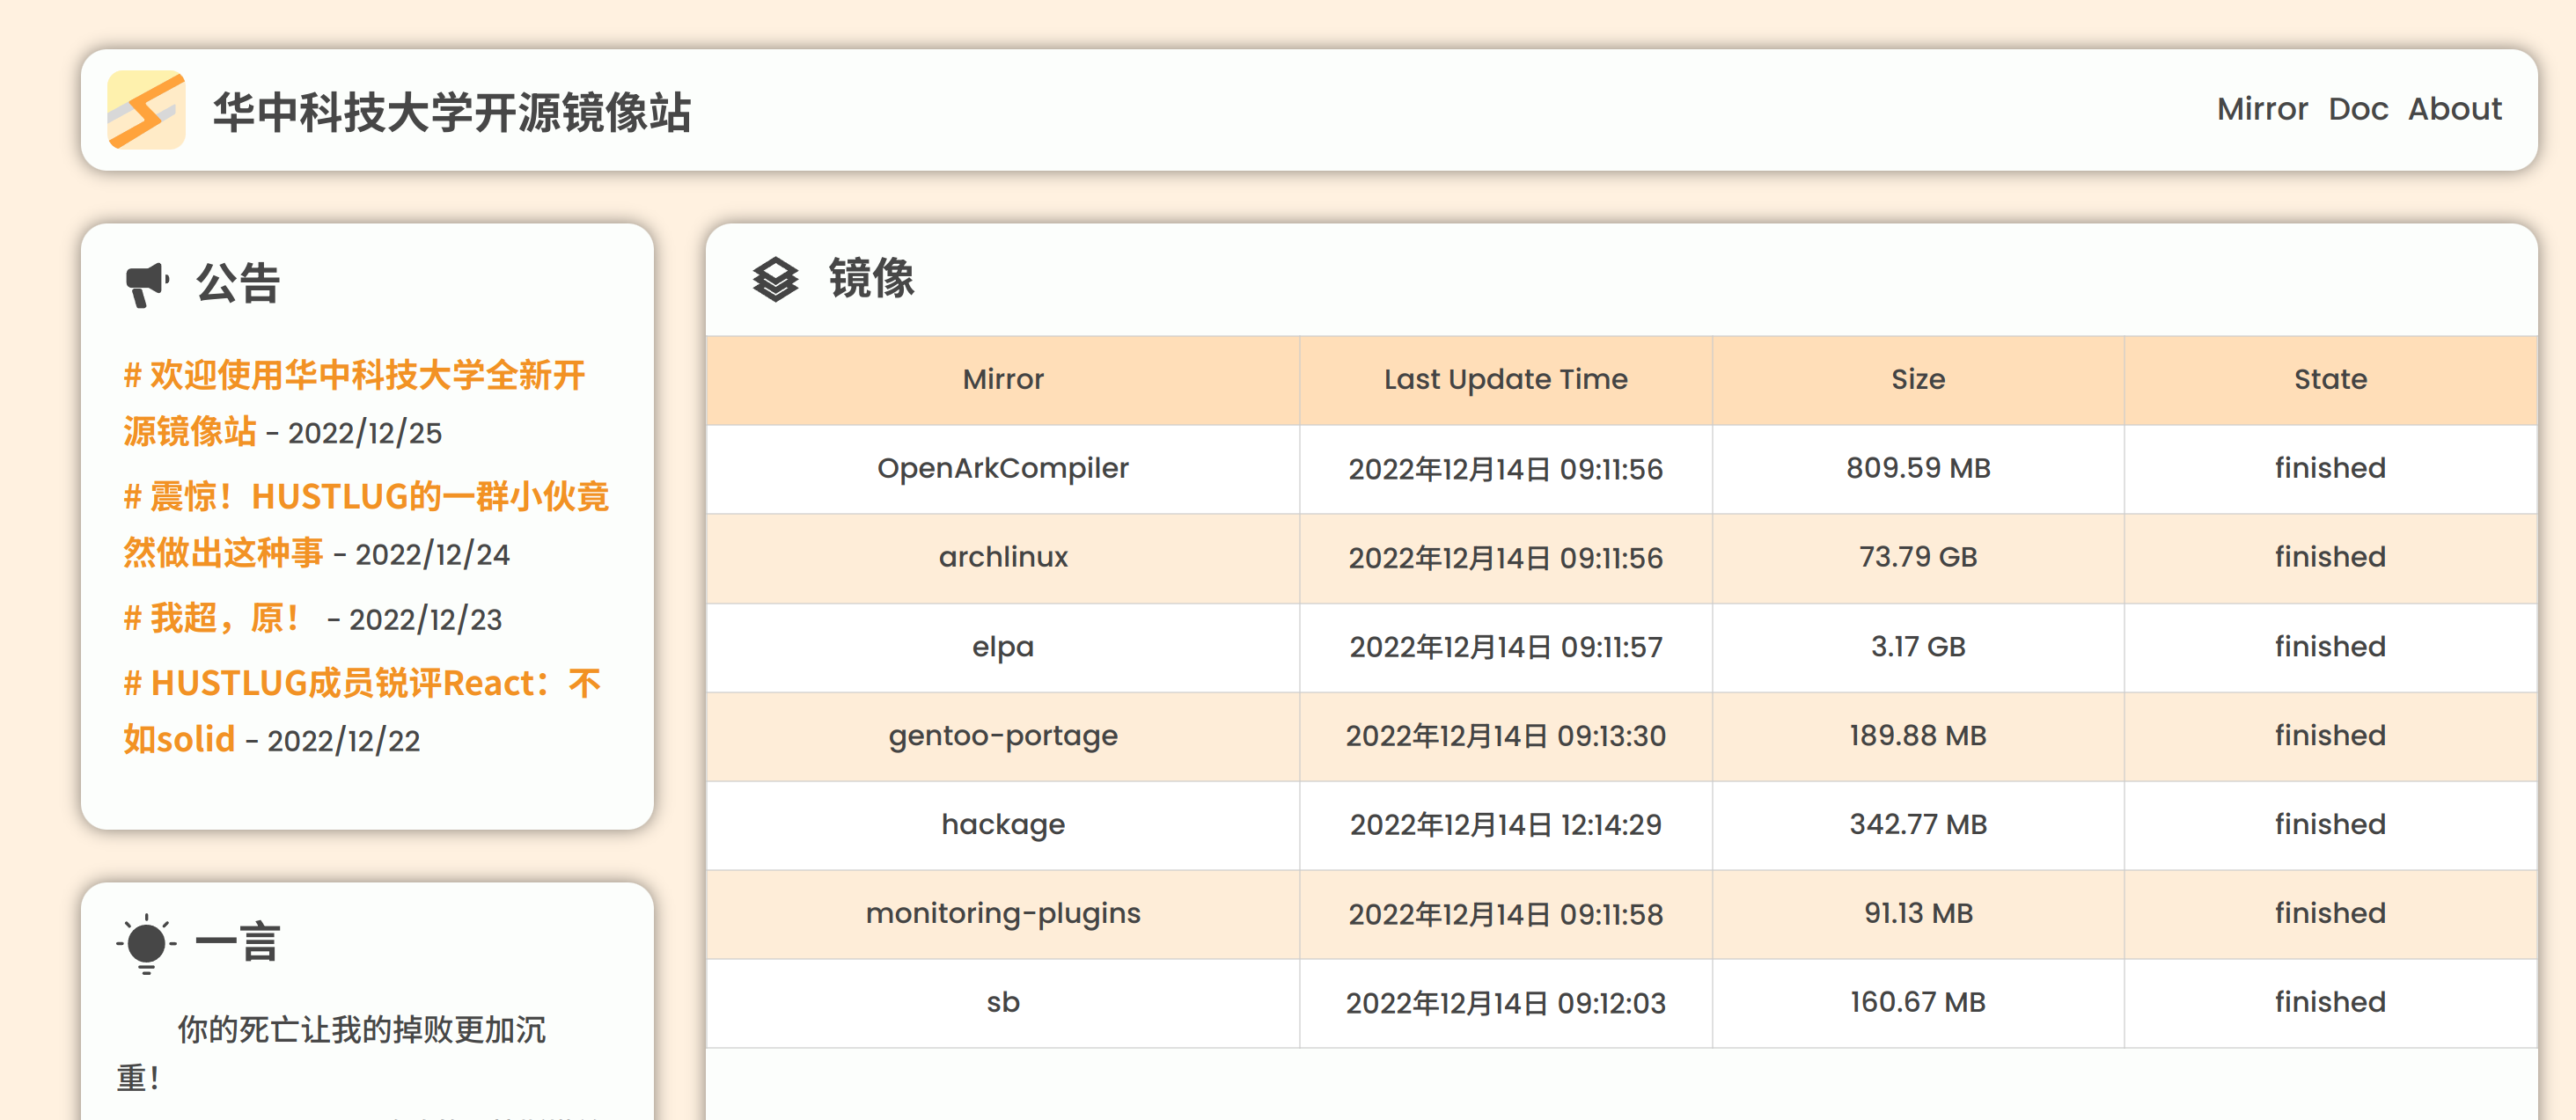
\includegraphics[width=1\textwidth]{./images/front.png}
    \caption{镜像站界面}
    \label{front}
\end{figure}

同时用户请求增加部分软件源
\begin{figure}[!h]
    \centering
    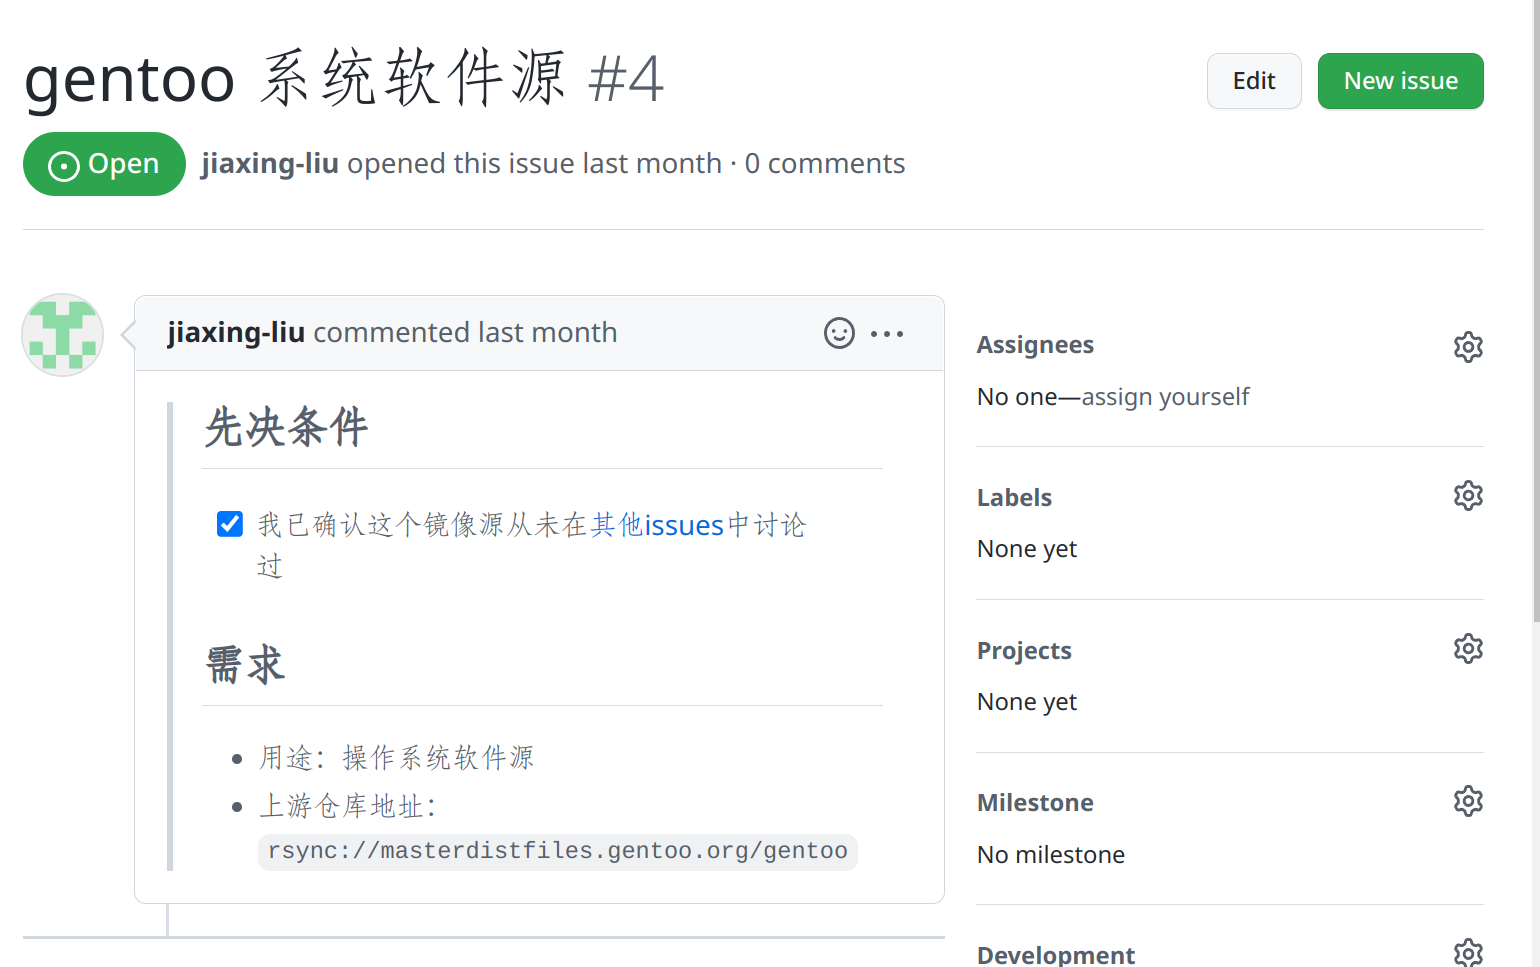
\includegraphics[width=0.7\textwidth]{./images/comment.png}
    \caption{用户提出的issue}
    \label{issue}
\end{figure}

对于前端编写的election应用,暂时没有进行用户测试,因为很多发行版是滚动发行版,在滚动更新中
可以导致系统出现异常,等到应用以及软件源稳定后再发布release供各个发行版用户使用。

\subsection{总结}
\begin{itemize}
    \item 使用iris搭建了web框架,同时搭建了完整的日志框架和日志分级机制。
    \item 使用xorm和postgresql完成了对数据的管理
    \item 编写了drone.yml进行了持续集成的操作
    \item 使用k8s技术使得服务部署更加方便
    \item 使用electron编写了跨平台的桌面应用
\end{itemize}

\section{体会}

程家骏同学:进行前后端开发的工作,在前端开发中其实遇到了很多问题,比如在安装中如何获取root权限的问题,
通过在archlinuxcn社区中提问得到的建议是持续的输入密码,防止root权限过期,最终我选择是编写shell脚本,进行自动化的
交互输入脚本。

在前端的后续开发中我发现原生js的开发难度过大,选择后续的开发中使用react + antd对项目进行重构。

在后端的开发中遇到的问题是git的同步问题,一开始打算参考清华的策略,编写脚本进行同步,但是实现的很不优雅,他们后续甚至单独
使用一个repo存放每个软件源的脚本,后续在go社区中了解使用go-git进行处理,虽然写起来很不习惯,但是最终
还是参考着go-git的文档完成了程序。

\section{附录}
同步软件源核心代码
\begin{lstlisting}
// SyncOneMirror
//
//	@Description: 同步一个软件源
//	@param ctx iris.context参数
func SyncOneMirror(ctx iris.Context) {
        // 获取软件源名称
        name := ctx.PostValue("Name")
        syncHelper(name)
        ctx.Writef("ok")
    }
    

// SyncAllMirror
//
//	@Description:同步全部的软件源
//	@param ctx iris的context参数
func SyncAllMirror(ctx iris.Context) {
	mirrors, err := crud.GetAllMirror()
	if err != nil {
		log.Error(err)
		return
	}
	// 进行并发的操作
	done := make(chan int, len(mirrors))
	for _, mirror := range mirrors {
		mirror := mirror
		go func() {
			syncHelper(mirror.Name)
		}()
		done <- 1
	}
	for i := 0; i < len(mirrors); i++ {
		<-done
	}
}

// syncHelper
//
//	@Description: 进行软件源的同步
//	@param name 软件源的名字
func syncHelper(name string) {
	syncType, err, mirror := crud.GetMirrorSyncType(name)
	if err != nil {
		log.Error(err)
		return
	}
	log.Info("start sync the " + mirror.Name)
	err = syncType.StartSync(mirror.SourceURL, mirror.LocalURL)
	if err != nil {
		log.Error(err)
		return
	}
	log.Info("success sync the " + mirror.Name)
}

\end{lstlisting}

软件上传核心代码
\begin{lstlisting}
// UploadFile
//
//	@Description: 上传软件
//	@param did	开发者的id
//	@param localPath	存放的本地路径
//	@param filename	软件名
func UploadFile(did int, localPath string, filename string) {
	if crud.Exist(filename) == false {
		crud.InsertSoftware(db.Software{
			Did:        did,
			UpdateTime: time.Now(),
			Name:       filename,
			LocalUrl:   localPath,
		})
	}
	crud.UpdateSoftwareTime(filename)
}

func Upload(context iris.Context) {
	did := context.Params().Get("did")
	//获取上传文件的信息
	file, info, err := context.FormFile("file")
	if err != nil {
		iris.New().Logger().Info(err.Error())
		context.JSON(iris.Map{
			"status":  "0",
			"type":    "0",
			"message": "文件上传失败!",
		})
		return
	}
	//最后要关闭文件
	defer file.Close()

	//获取文件名称`
	fname := info.Filename
	id, _ := strconv.Atoi(did)
	localPath := "./uploads/" + fname
	UploadFile(id, localPath, fname)
	//把文件上传到哪里
	out, err := os.OpenFile(localPath, os.O_WRONLY|os.O_CREATE, 0666)
	if err != nil {
		iris.New().Logger().Info(err.Error())
		context.JSON(iris.Map{
			"status":  "0",
			"type":    "0",
			"message": "文件位置打开失败!",
		})
		return
	}

	//我们打印一下文件路径
	iris.New().Logger().Info("文件路径:" + out.Name())
	//最终也不要忘记关闭上传之后的文件流
	defer out.Close()

	//拷贝文件到指定位置
	_, err = io.Copy(out, file)
	if err != nil {
		context.JSON(iris.Map{
			"status":  "0",
			"type":    "0",
			"message": "文件上传彻底失败!",
		})
		return
	} else {
		context.JSON(iris.Map{
			"status":  "1",
			"type":    "1",
			"message": "文件上传成功!",
		})
	}
}
\end{lstlisting}

Dockerfile
\begin{lstlisting}
FROM golang:1.19.2-alpine3.16 AS builder
LABEL stage="go-builder"
ARG USE_GO_PROXY=1
WORKDIR /app
COPY ./ ./
RUN if [ $USE_GO_PROXY -eq 1 ]; then \
        go env -w GO111MODULE=on && \
        echo "Using go proxy" && \
        go env -w GOPROXY=https://mirrors.cloud.tencent.com/go,direct; \
    fi; \
    go mod tidy && go build -o ./bin/hust-sync ./src/app

FROM alpine:edge
LABEL stage="go-runner"
VOLUME /app/hust-sync/log
VOLUME /app/hust-sync/mirror
WORKDIR /app/hust-sync
COPY --from=builder /app/bin/hust-sync ./
RUN apk add --no-cache rsync tzdata
EXPOSE 3000
CMD ["./hust-sync"]


\end{lstlisting}
前端解析软件源数据
\begin{lstlisting}
import json
from pdb import line_prefix
import readline
import string

f = open("data/temp")

dicts = []
line = f.readline()
while line:
    strings = line.split(' ')
    print(strings)
    temp = strings[0][6:]
    # 获取名字和版本
    dicts.append({"name": temp, "version": strings[1].replace('\n','')})
    line = f.readline()
    line = f.readline()
dicts = json.dumps(dicts)
f.close()
w = open("data/local_package.json", 'w')
w.write(dicts)
\end{lstlisting}
\end{document}
